\documentclass[12pt, a4paper]{article}


% --- 核心宏包 ---
\usepackage{graphics}
\usepackage{float}
\usepackage[UTF8]{ctex}        % 中文支持
\usepackage{geometry}         % 页面边距
\usepackage{graphicx}         % 插入图片
\usepackage{amsmath, amssymb} % 数学公式
\usepackage{setspace}         % 行间距
\usepackage{titlesec}         % 标题格式定制
\usepackage{booktabs}         % 三线表
\usepackage{hyperref}         % 超链接
\usepackage{multirow}         % 多行表格
\usepackage{array}            % 表格列格式
\usepackage{listings}         % 代码高亮
\usepackage{xcolor}           % 颜色
\usepackage[backend=biber, style=gb7714-2015]{biblatex}
\addbibresource{refs.bib}

% --- 页面设置 ---
\geometry{left=3.18cm, right=3.18cm, top=2.54cm, bottom=2.54cm}
\onehalfspacing

% --- 标题格式设置 ---
\titleformat{\section}{\large\bfseries}{\thesection}{1em}{}
\titleformat{\subsection}{\normalsize\bfseries}{\thesubsection}{1em}{}
\titleformat{\subsubsection}{\normalsize\bfseries}{\thesubsubsection}{1em}{}

% --- 代码环境 ---
\lstset{
  basicstyle=\small\ttfamily,
  keywordstyle=\color{blue},
  commentstyle=\color{gray},
  numbers=left,
  numberstyle=\tiny\color{gray},
  frame=single,
  breaklines=true,
  captionpos=b
}

\begin{document}

% --- 封面 ---
\begin{center}
	
\includegraphics[width=0.8\textwidth]{figures/XJTU_2024.png}
	\vspace*{1.5cm}
	\newline
	{\LARGE \textbf{面向边缘智能应用的Int8数字存算一体架构设计及FPGA验证}} \\[2cm]

	\vspace*{3cm}

	\begin{spacing}{2.0}
		\begin{tabular}{ll}
			\textbf{学 \quad 号：} & 2221411116                                                                   \\
			\textbf{姓 \quad 名：} & 焦宏宝                                                                          \\
			\textbf{导 \quad 师：} & 梁峰                                                                           \\
			\textbf{论文题目：}      & \begin{tabular}[t]{l} 面向边缘智能应用的Int8 -- \\ 数字存算一体架构设计及FPGA验证 \end{tabular} \\
			\textbf{专 \quad 业：} & 微电子科学与工程 强芯实验班                                                               \\
			\textbf{学 \quad 院：} & 电信学部　微电子学院                                                                   \\
			\textbf{填写时间：}      & 2026年 05月
		\end{tabular}
	\end{spacing}
\end{center}

\newpage

% --- 摘要 ---
\begin{center}
	{\large\bfseries 摘\quad 要}
\end{center}

随着深度学习在边缘智能场景中的广泛部署，传统冯·诺依曼架构中处理器与存储器分离所带来的数据搬运瓶颈日益突出。存算一体（Computing-in-Memory, CIM）技术通过在存储阵列内部或近存储位置完成计算，从体系结构层面缓解"内存墙"问题，被认为是提升推理能效与吞吐率的重要方向。

本文设计并实现了一种面向边缘推理的INT8数字存算一体矩阵计算阵列架构，并在PYNQ-Z2（Zynq-7020）FPGA平台上完成了完整的综合部署与板级验证。系统以16×16 CIM Tile为原子计算单元，采用参数化设计支持可配置并行度，核心引擎通过多级流水线状态机实现权重加载、零点减法、MAC运算、偏置累加、ReLU激活、重量化与结果写回的完整推理数据通路，最终使计算阵列支持对任意由全连接层，卷积计算层以及简单激活函数组成的模型的计算。在数据通路方面，设计了AXI4-Stream + DMA的双向批量传输架构替代传统逐字MMIO，将数据搬运效率提升两个数量级；在存储子系统方面，通过输入/输出缓冲双bank乒乓结构实现了DMA传输与硬件计算的重叠执行，有效隐藏了数据搬运延迟；针对连续全连接层，设计了OBUF→IBUF内部硬件直拷的层融合机制，消除了层间DMA往返开销。在软件侧，引入了块对角权重打包（SQ-mapping）的卷积映射优化方法，并将其适配到本设计的数据通路上，把稀疏小卷积核的CIM阵列利用率从不足5\%提升至接近100\%。

在控制路径方面，集成了PicoRV32 RISC-V软核替代ARM PS进行推理控制，通过总线桥接实现与CIM IP完全兼容的AXI事务，配合双端口BRAM实现运行时固件加载与结果回读，使CIM加速器可在纯PL侧自主运行。

实验结果表明，本设计在100 MHz工作频率下，MLP网络（784→128→10）端到端延迟为2.00 ms/幅（499.6 fps，DMA+batch模式），LeNet-5 CNN（7层）端到端延迟为29.91 ms/幅（33.4 fps），相对AXI4-Lite逐字MMIO基线在相同100 MHz频率下实现约109倍累计加速，200张MNIST测试图片分类准确率99.5\%，全部输出与Python bit-accurate参考模型逐元素一致。PicoRV32控制模式以100 在100 MHz下时序轻微违例（WNS=$-$0.694 ns）但常温上板功能正确，且呈现出显著的轻量化优势：相比ARM模式反而减少351个LUT（17,023 vs 17,374）和2,317个FF（8,594 vs 10,911），仅增加6个BRAM用于固件/结果存储，以更少的逻辑资源实现了纯PL侧自主推理，200张图片验证准确率96.50\%且全部logits与ARM路径bit-exact一致。系统占用LUT 32.66\%、BRAM 88.21\%、DSP 100\%，CIM IP动态功耗为0.559 W。

\vspace{1em}
\noindent\textbf{关键词：}存算一体；INT8量化推理；FPGA验证；CIM阵列；AXI4-Stream DMA；双缓冲；PicoRV32

\newpage

% --- Abstract ---
\begin{center}
	{\large\bfseries ABSTRACT}
\end{center}

With the widespread deployment of deep learning at the edge, the data movement bottleneck caused by the separation of processor and memory in traditional von Neumann architectures has become increasingly prominent. Computing-in-Memory (CIM) technology mitigates the "memory wall" problem at the architectural level by performing computation within or near memory arrays, and is considered a promising direction for improving inference energy efficiency and throughput.

This thesis designs and implements an INT8 digital computing-in-memory matrix computation array architecture for edge inference, with complete synthesis, deployment and board-level verification on the PYNQ-Z2 (Zynq-7020) FPGA platform. The system employs a 16$\times$16 CIM Tile as the atomic compute unit with parameterizable parallelism. The core engine implements a multi-stage pipelined FSM covering the complete inference datapath: weight loading, zero-point subtraction, MAC operation, bias accumulation, ReLU activation, requantization, and result writeback, ultimately enabling the compute array to support arbitrary models composed of fully-connected layers, convolutional layers, and simple activation functions. For the data path, an AXI4-Stream + DMA bidirectional bulk-transfer architecture replaces conventional per-word MMIO, improving data movement efficiency by two orders of magnitude. In the memory subsystem, input/output buffer double-bank ping-pong structures overlap DMA transfers with hardware computation, effectively hiding data movement latency. For consecutive fully-connected layers, an OBUF$\rightarrow$IBUF internal hardware copy mechanism (layer fusion) eliminates inter-layer DMA round-trips. On the software side, a block-diagonal weight packing method (SQ-mapping) is adopted and adapted to the proposed datapath to improve CIM array utilization for sparse small-kernel convolutions from below 5\% to near 100\%.

For the control path, a PicoRV32 RISC-V soft-core is integrated to replace the ARM PS for inference control. A bus bridge issues AXI transactions fully compatible with the CIM IP, and dual-port BRAMs enable runtime firmware loading and result readback, allowing the CIM accelerator to operate autonomously in pure programmable logic.

Experimental results show that at 100 MHz, the MLP network (784$\rightarrow$128$\rightarrow$10) achieves 2.00 ms/image end-to-end (499.6 fps, DMA+batch mode), while LeNet-5 CNN (7 layers) achieves 29.91 ms/image end-to-end (33.4 fps), representing an approximately 109$\times$ cumulative speedup over the AXI4-Lite per-word MMIO baseline at the same 100 MHz, with 99.5\% classification accuracy on 200 MNIST test images and full bit-exact agreement with the Python bit-accurate reference model. The PicoRV32 control mode runs functionally correctly at 100 MHz with marginal timing (WNS=$-$0.694 ns) and demonstrates a notable lightweight advantage: it actually uses 351 fewer LUTs (17,023 vs 17,374) and 2,317 fewer FFs (8,594 vs 10,911) than the ARM mode, while adding only 6 BRAMs for firmware/result storage, achieving autonomous inference in pure programmable logic with fewer logic resources, delivering 96.50\% accuracy on 200 images with all logits bit-exact to the ARM path. The system utilizes 32.66\% LUTs, 88.21\% BRAM, and 100\% DSP, with the CIM IP consuming 0.559 W dynamic power.

\vspace{1em}
\noindent\textbf{KEY WORDS:} Computing-in-Memory; INT8 quantized inference; FPGA verification; CIM array; AXI4-Stream DMA; double buffering; PicoRV32

\newpage

% --- 目录 ---
\tableofcontents
\newpage

% ====================================================================
\section{绪论}
% ====================================================================

\subsection{选题背景}

近年来，以YOLO\cite{10}、SSD\cite{11}为代表的深度学习目标检测算法在智能安防、工业视觉、无人系统与车载感知等场景中被广泛采用，其共同特点是需要在较高精度下实现接近实时的推理能力，而网络内部又以卷积/矩阵乘加（MAC）为主导计算负载，导致整体计算量与数据访问量都十分庞大。YOLO将检测任务端到端地建模为单网络回归问题，SSD则是通过多尺度特征图上的卷积预测实现单阶段检测，这类方法在追求速度与精度的同时，也使得卷积算子成为系统性能与功耗优化的核心瓶颈之一。


\begin{figure}[H]
	\centering
	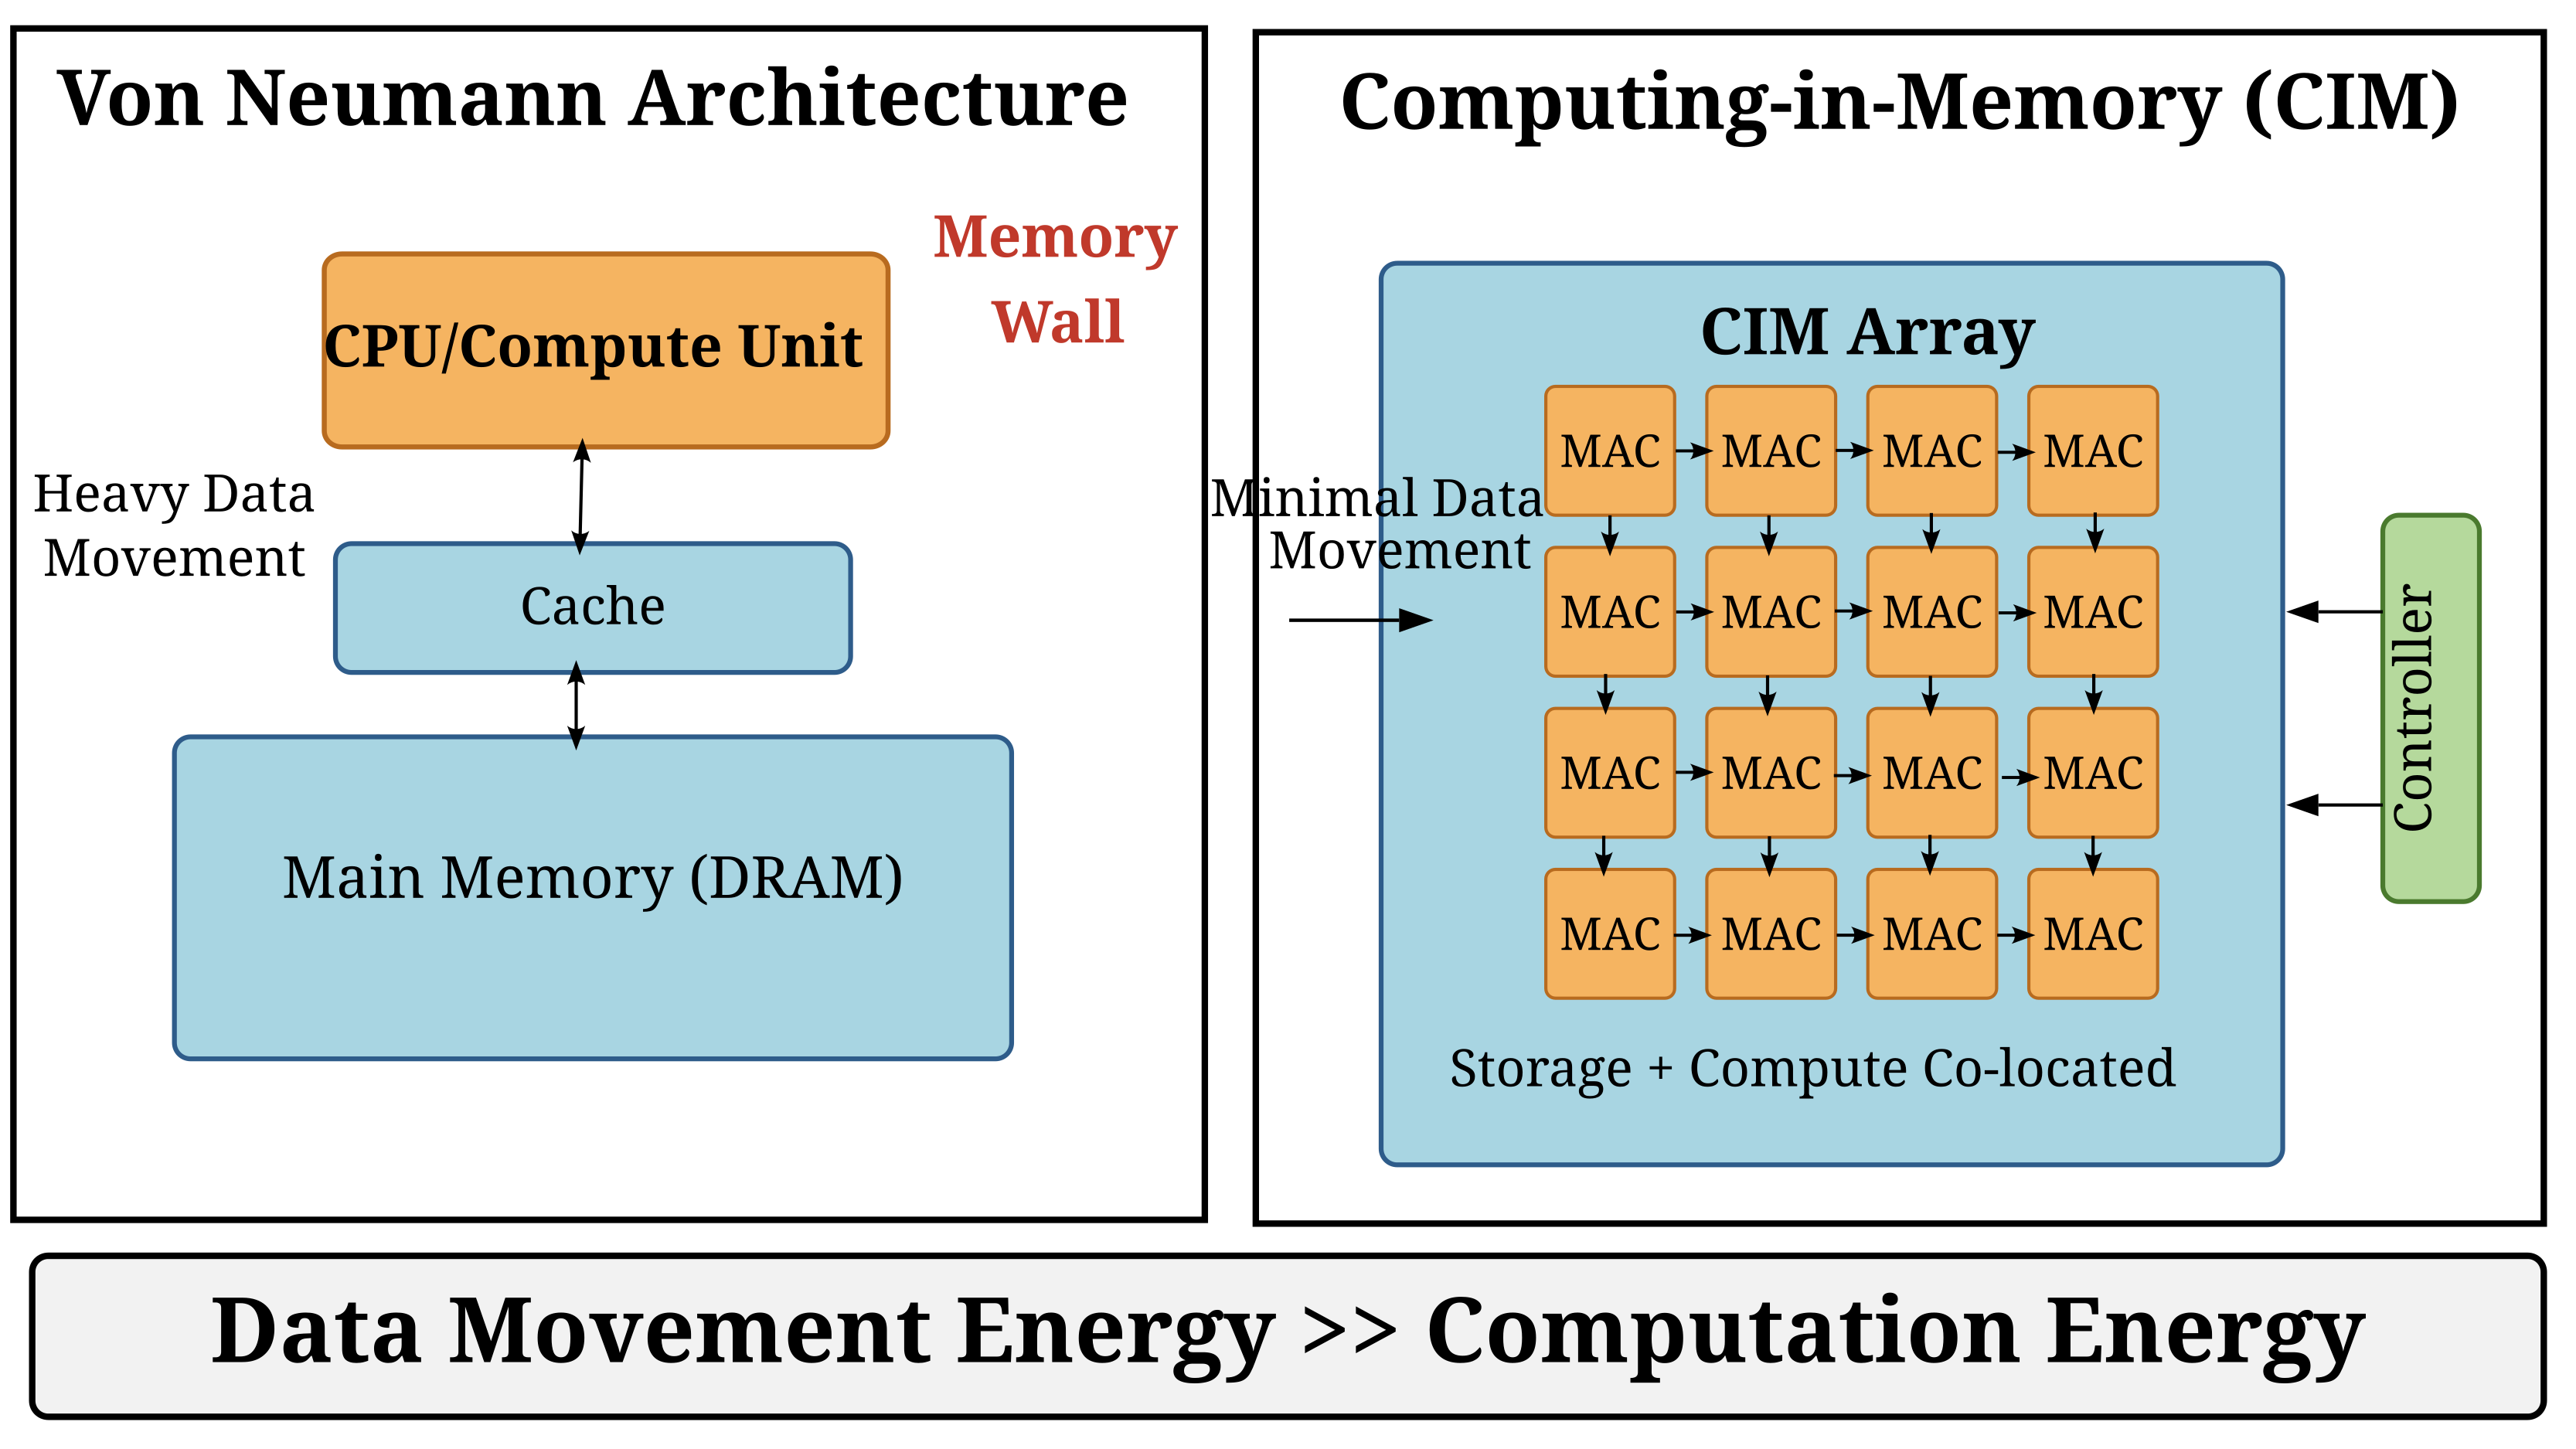
\includegraphics[width=0.92\textwidth]{pics/1-1.png}
	\caption{冯·诺依曼架构与存算一体架构对比示意图。左侧传统架构中计算单元与存储器分离，数据需在层级间频繁搬运，受"内存墙"制约；右侧存算一体架构将计算单元嵌入存储阵列内部，实现存储与计算的位置协同，显著减少数据搬运。}
	\label{fig:vn_vs_cim}
\end{figure}

然而，在传统冯·诺依曼架构中，处理器与存储器相互分离，权重与特征图等数据需要在存储层级与计算单元之间频繁搬运，导致数据搬运资源开销远比实际计算要大，系统性能逐渐受限于存储带宽与访问延迟，"内存墙（Memory Wall）"问题由此形成并长期存在（如图\ref{fig:vn_vs_cim}所示）。Wulf与McKee早在1995年就指出处理器速度提升与存储器速度提升之间的差距会不断扩大，从而限制系统级性能提升\cite{1}。与此同时，能效维度的矛盾更加突出：在先进工艺条件下，数据搬运（尤其是跨层级、跨片外存储访问）相对于算术运算存在着显著更高的能量代价，使得"算得快"并不等价于"算得省"。Horowitz在ISSCC 2014的报告中系统讨论了计算系统的能耗拆分，强调需要从体系结构与数据流层面减少昂贵的数据访问\cite{2}。面向CNN的专用加速器研究也进一步表明：通过数据复用与数据流优化降低（尤其是片外）访存开销，是实现低功耗实时推理的关键路径之一\cite{3}。在边缘计算场景（比如电池供电、散热受限和实时性要求较高的场景）中，上述矛盾更加尖锐，传统"分离式计算-存储"模式难以同时满足吞吐与能效需求。图\ref{fig:energy_per_op}对比了典型算术运算与不同层级存储访问的单次操作能耗（对数坐标，45nm工艺典型值\cite{2}），可见片外DRAM访问的能耗比一次8-bit MAC运算高出约两个数量级，直观地解释了想要实现低功耗推理为何要同时降低数据搬运而非单纯提升算力。

\begin{figure}[H]
	\centering
	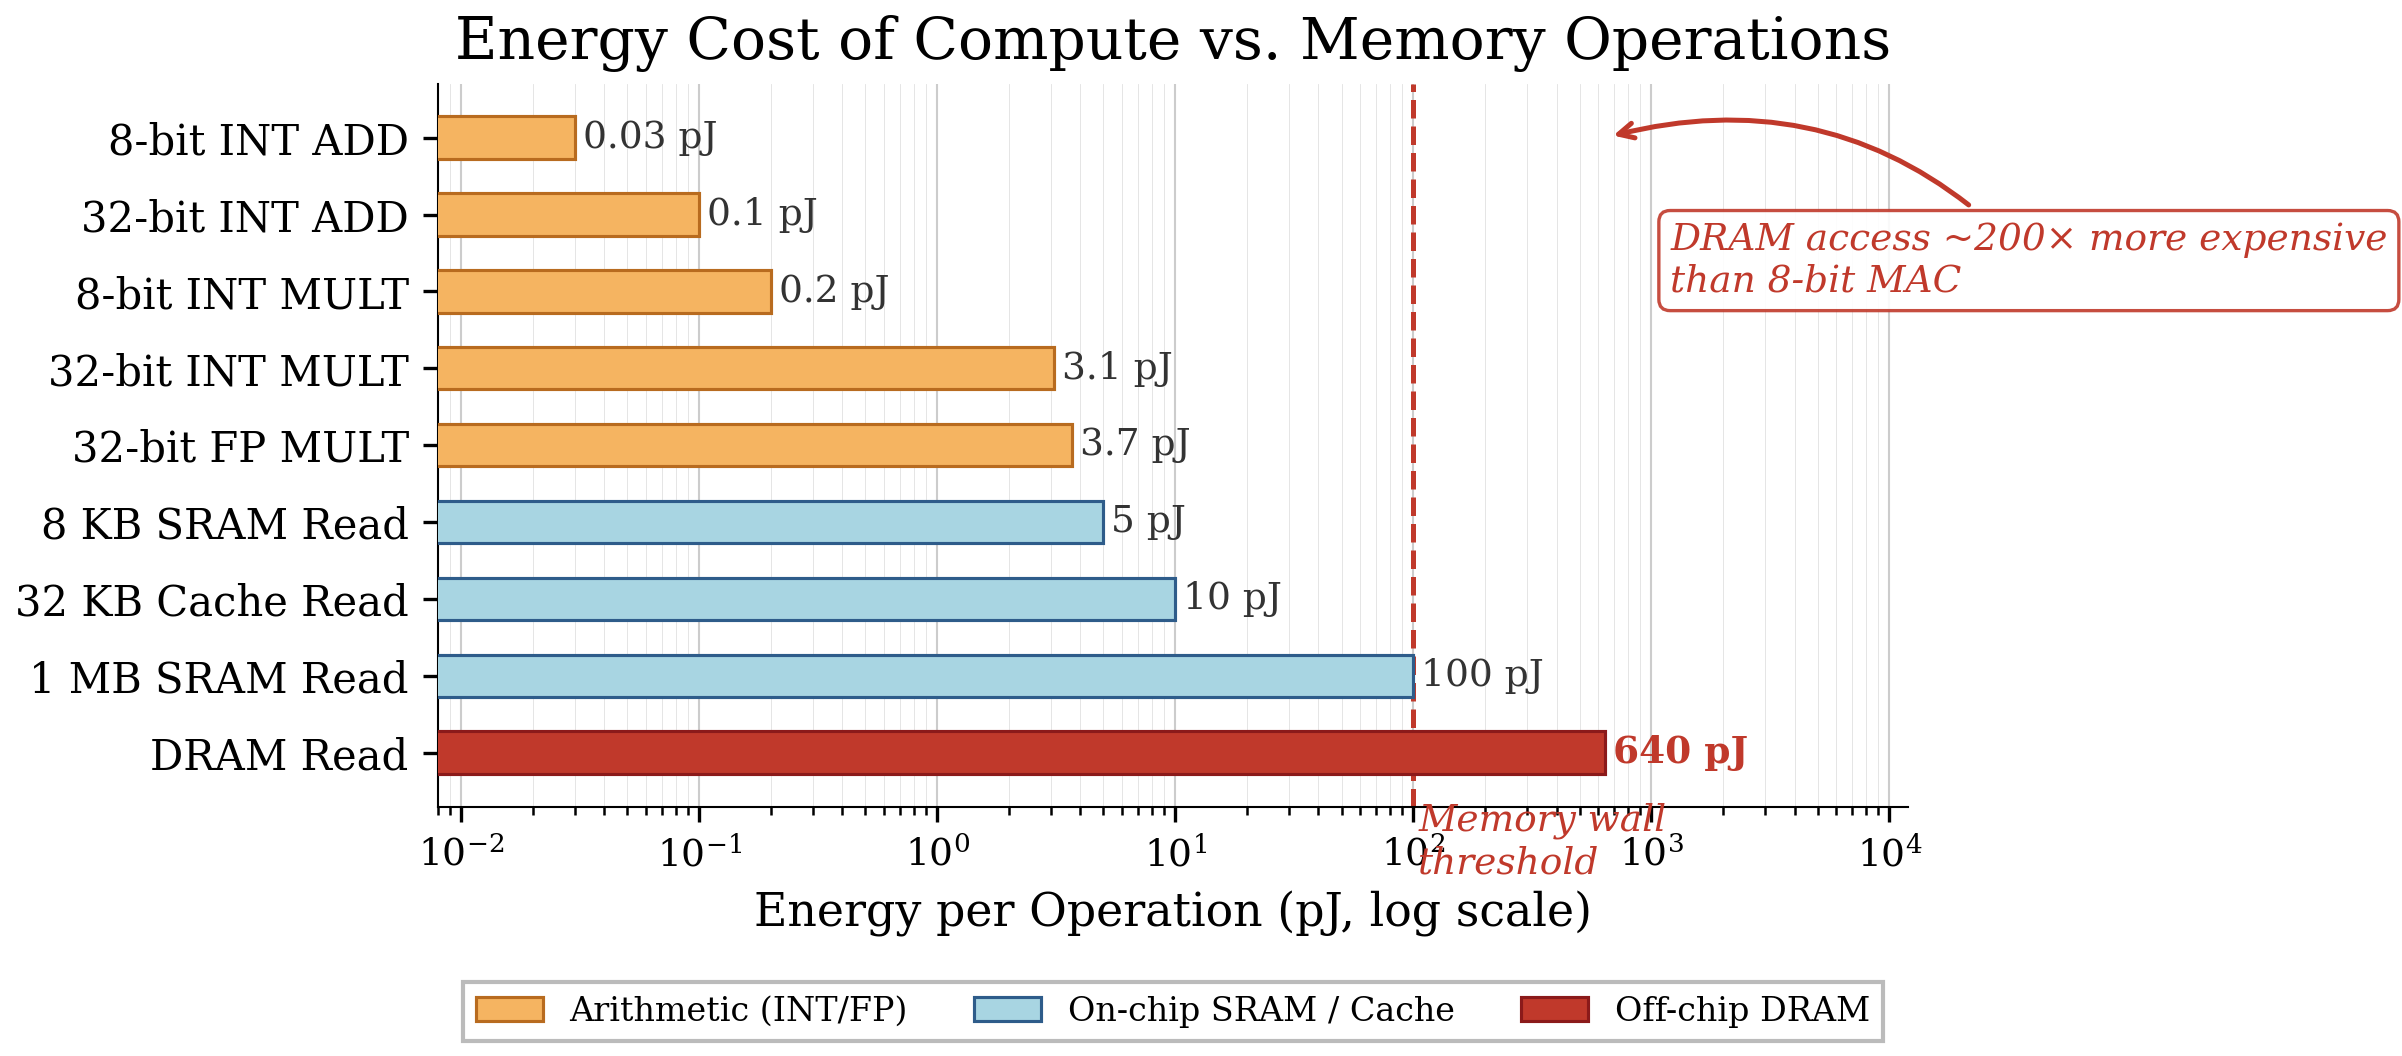
\includegraphics[width=0.85\textwidth]{pics/1-2.png}
	\caption{计算与存储操作的单次能耗对比（pJ，对数坐标）。算术运算（橙色）能耗显著低于片上SRAM/Cache访问（蓝色），而片外DRAM访问（红色）的能耗最高；数据搬运的能量代价是边缘推理需要重点优化的对象。}
	\label{fig:energy_per_op}
\end{figure}

存算一体（Computing-in-Memory, CIM）技术通过在存储阵列内部或近存储位置完成计算，将"数据搬运"转化为"原位计算"，从体系结构层面缓解冯·诺依曼瓶颈。Nature Electronics的一些综述工作提出了覆盖不同存储器参与程度的CIM全谱系分类框架，并指出CIM可在逻辑运算与乘加运算等基本原语上实现能效提升\cite{4}。在诸多实现路径中，基于标准CMOS工艺的SRAM-CIM具有速度快、工艺成熟、可靠性高、与主流数字设计流程兼容等优点，是面向工程落地与系统集成的重要路线之一\cite{5}。Chuan-Jia Jhang团队系统综述了SRAM-CIM在AI边缘设备中的挑战与发展趋势\cite{30}，司鑫与Dong Fangyuan团队也从设计挑战与方法学角度对SRAM-CIM进行了全面回顾\cite{31}\cite{34}。目前来讲，CIM技术被认为是突破内存墙、提升能效与吞吐率的重要方向。

从应用角度看，为在精度、硬件复杂度与系统吞吐之间取得平衡，Int8量化推理已成为工业界与学术界常用的落地方案之一。Jacob等人提出的整数算术推理量化方法表明，通过合理的量化尺度与训练以及恰当的校准策略，可在保持精度的前提下实现高效的整数运算推理流程\cite{6}。从硬件角度看，已有研究在SRAM-CIM宏单元中展示了面向多比特MAC的实现范式，如8b MAC的SRAM CIM宏以及支持Signed-INT8的SRAM CIM宏等工作，说明"多比特、可用于实际推理精度需求"的SRAM-CIM在工程上具有可行性\cite{8}\cite{32}。另外，在硬件加速方面，FPGA因其可重构性、低延迟与较高的能效比，已成为神经网络推理加速的重要平台\cite{meng2025}，已有工作在此基础上探索了注意力机制等特定算子的FPGA硬件加速\cite{feng2024}。

基于上述背景，本课题面向边缘智能推理的能效与实时性需求，在标准CMOS SRAM工艺假设下，设计了一种支持Int8数据类型的数字存算一体矩阵计算阵列架构（设计空间定位与两种实现极端的分析见§\ref{sec:two_extremes}）：在存储阵列内实现权重存储与乘法以及部分积生成，结合合理的阵列并行组织、累加与数据通路调度，降低数据搬运开销并提升并行吞吐；通过Synopsys公司的VCS工具完成仿真测试，在AMD公司的Vivado(2024.2版本)完成综合和布局布线，并在FPGA平台完成实际综合部署与功能验证，形成了可复现的验证平台与完整代码交付。

\subsection{国内外现状及发展趋势}

存算一体研究近年来快速发展，已形成覆盖器件/电路/架构/算法的多层次技术体系。相关工作从实现介质（SRAM、DRAM、RRAM/PCM等）与计算形态（模拟/数字、阵列内/近存储）对CIM进行系统分类，指出其共同目标是减少访存与数据移动开销、利用阵列并行来提升吞吐\cite{4}\cite{5}\cite{12}\cite{14}\cite{30}\cite{31}\cite{34}。图\ref{fig:cim_taxonomy}按存储介质与计算形态给出了CIM技术的谱系分类，并标注了各分支的代表性工作；本文的设计落在"SRAM-CIM → 数字SRAM-CIM"这一分支（图中红框高亮），与ReDCIM、TranCIM、MulTCIM等数字CIM工作处于同一技术路线。

\begin{figure}[H]
	\centering
	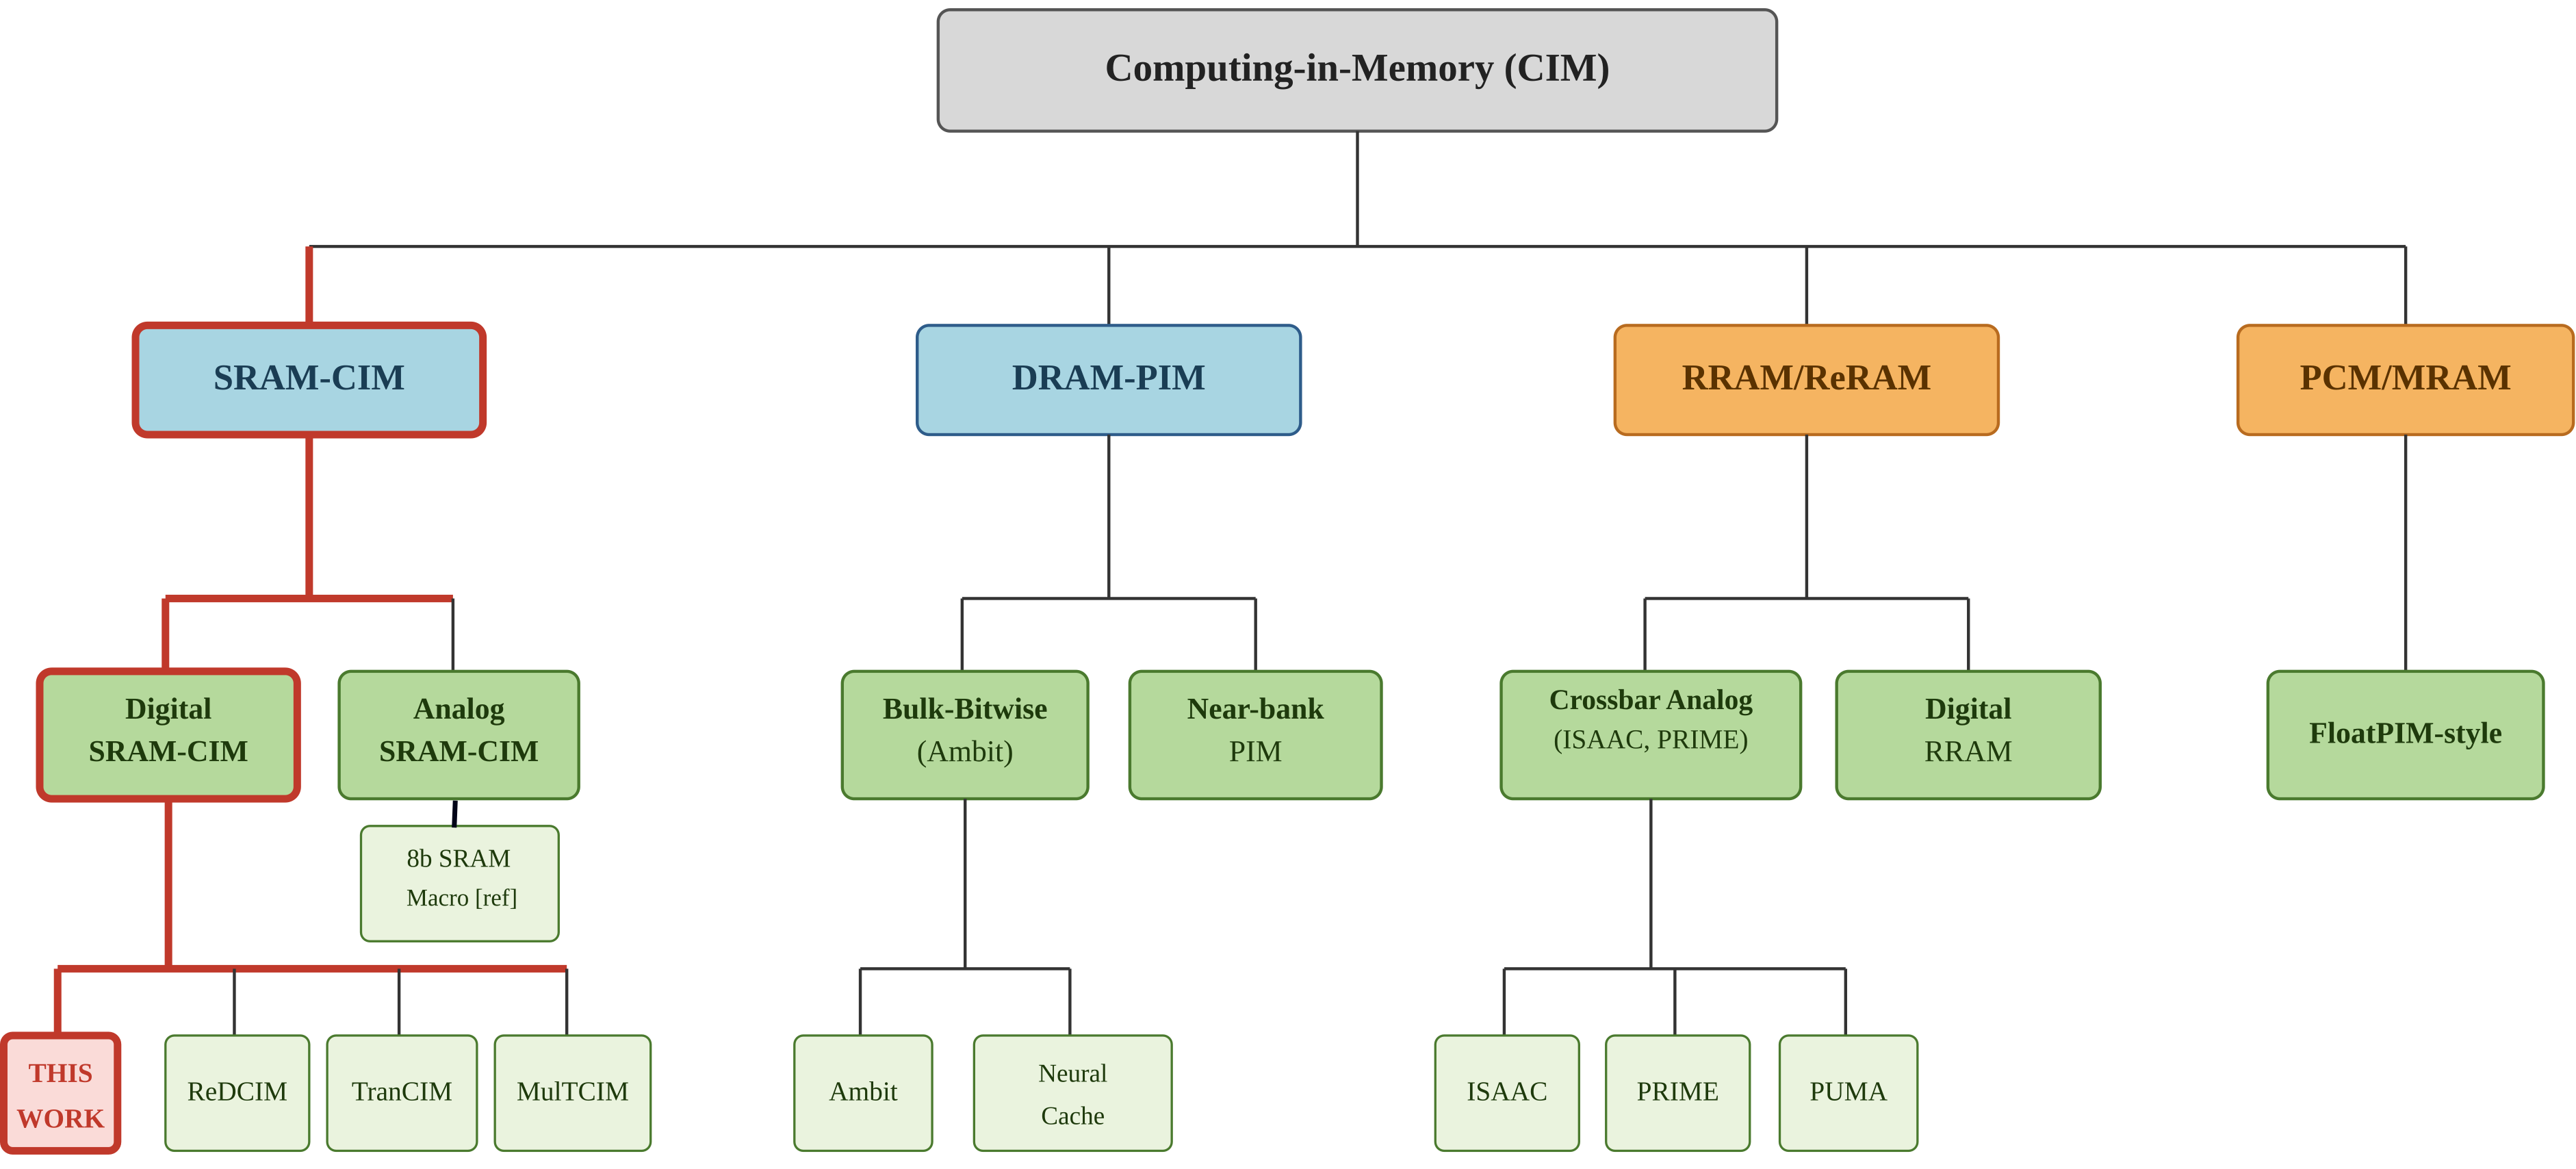
\includegraphics[width=0.95\textwidth]{pics/1-3.png}
	\caption{存算一体技术分类谱系图。按存储介质（SRAM/DRAM/RRAM/PCM等）与计算形态（模拟/数字、阵列内/近存储）划分，叶节点为各分支代表性工作。本文工作位于数字SRAM-CIM分支（红框高亮）。}
	\label{fig:cim_taxonomy}
\end{figure}

在国际研究中，基于新型非易失存储器（如RRAM）交叉阵列的模拟CIM方案曾是重要热点，典型代表包括ISAAC\cite{17}和PRIME\cite{18}等工作。PUMA等可编程memristor加速器进一步探索了可编程的推理加速路径\cite{19}。但模拟CIM往往需要ADC/DAC等外围电路并面临器件非理想性、噪声等的影响，其精度与可校准性面临不小的挑战\cite{4}\cite{15}。面向通用存储体系的近存储计算也形成了多条路线，如Ambit\cite{21}、Neural Cache\cite{20}、FloatPIM\cite{22}等。

在电路与工程实现层面，基于标准CMOS工艺的SRAM-CIM因其速度、成熟度与数字设计流程兼容性而成为当前研究与产业化的重要路线\cite{5}\cite{12}\cite{14}。已有多项芯片级宏单元工作给出了可参考的实现范式，比如在28nm工艺下实现的64Kb 6T SRAM-CIM宏单元\cite{32}，以及支持Signed-INT8的ADC-less SRAM-CIM宏单元\cite{8}。研究趋势正从"单个CIM宏单元验证"走向"可重构/可编程的数字CIM处理器与系统级加速器"。涂锋斌老师团队提出了支持BF16与INT8的可重构数字CIM处理器\cite{24}，其后续ReDCIM工作给出了统一FP/INT的数字CIM设计\cite{25}。同期也出现面向Transformer/注意力工作负载的数字CIM加速研究，如TranCIM\cite{26}、MulTCIM\cite{27}等。

在算法侧，Int8量化推理已成为常用的落地路径。Jacob等工作提出的整数算术推理量化方法提供了硬件采用Int8数据通路的算法依据\cite{6}。PACT\cite{28}与LSQ\cite{29}等研究进一步从训练与量化参数学习角度改善量化精度。在能效方面，Dong Qing等在7nm FinFET工艺下实现了351 TOPS/W的SRAM-CIM宏单元\cite{33}，展现了先进工艺下CIM的巨大能效潜力。

综合来看，国内外CIM研究呈现如下趋势：技术路线从"模拟/新型器件主导"扩展为"模拟与全数字并行发展"；算子与精度从低比特走向多比特MAC（尤其是Signed-INT8）；应用从CNN拓展到Transformer/多模态；验证方式越来越需要体系结构层面的可复现评估（包括RTL/FPGA原型验证、资源/频率/吞吐/延迟评估等）\cite{12}\cite{16}。本课题正是在此背景下，以数字SRAM-CIM阵列架构为核心，围绕数据通路、控制调度与FPGA验证建立了工程闭环。

\subsection{本文主要工作与贡献}

本文完成了以下工作：

（1）设计并实现了参数化的16×16 INT8 CIM Tile阵列与多级流水线加速器核心，支持可配置并行度（PAR\_OB参数）与Tile内MAC拆分因子（TILE\_SPLIT\_FACTOR），在单一FSM引擎中处理任意层的MVM运算。

（2）设计了完整的AXI4-Stream + DMA双向数据通路：MM2S方向实现权重/输入/偏置的批量加载，S2MM方向实现推理结果的DMA回读，将数据搬运效率相对逐字MMIO提升两个数量级。在此基础上，实现了输入/输出缓冲双bank乒乓结构，将DMA传输与硬件计算重叠执行，有效隐藏数据搬运延迟。

（3）针对连续全连接层场景，设计了OBUF→IBUF内部硬件直拷的层融合（Layer Fusion）机制，消除FC→FC层间的S2MM+MM2S DMA往返，并结合权重/偏置基址偏移实现多层权重共存与批量推理。

（4）在软件侧引入并适配了块对角权重打包（SQ-mapping）的卷积映射方法，通过将多个输出像素的im2col列与复制权重合并到同一次MVM调用，将稀疏小卷积核场景下的CIM阵列利用率从不足5\%提升至接近100\%。需要说明的是，SQ-mapping本身是已有的卷积映射技术，本文的工作在于将其与本设计的硬件维度上限、双缓冲乒乓批处理与层融合数据通路相结合并完成工程落地与验证。

（5）解决了权重SRAM的BRAM推断问题：将2048位宽的weight SRAM拆分为16个独立的128位bank，确保Vivado成功推断为BRAM；设计了read-modify-write式的AXI写入通路，在保持32位AXI接口的同时实现128位整行写入。

（6）集成PicoRV32 RISC-V软核替代ARM PS进行推理控制，设计了总线桥接、双端口FW/Result BRAM等模块，实现了纯PL侧自主推理能力。

（7）建立了"Python golden model → VCS仿真 → PYNQ上板"三层一致的验证方法，在PYNQ-Z2平台上完成了MLP和LeNet-5 CNN的端到端验证，全部输出与软件参考模型bit-exact一致，并提供了完整的性能评估数据。

% ====================================================================
\section{INT8 CIM阵列架构设计}
% ====================================================================

\subsection{数字SRAM-CIM的两种实现极端与本设计定位}
\label{sec:two_extremes}

在进入具体的模块设计之前，有必要先界定本课题在整个数字SRAM-CIM设计空间中的位置。现有数字SRAM-CIM的实现方式虽然种类繁多，但若按"单个存储位参与计算的粒度"这一维度来观察，可以抽象出两种典型的实现极端：一端是\textbf{比特级bit-serial popcount}架构，另一端是\textbf{字级行为建模MAC}架构。理解这两端的权衡，有助于解释为什么本课题在PYNQ-Z2资源约束下选择了后者。

\subsubsection{一：比特级 bit-serial popcount 架构}

这种架构把存储单元直接用作一位乘法器。该架构的典型形态是：SRAM cell只存储1位权重$w_i$，输入$x_i$的一位以WL广播进入阵列，BL/BLB上得到$x_i \cdot w_i$（实质是AND运算），再由阵列底部的加法器树对一整列做popcount累加得到一位×一位的点积。为支持INT8精度，输入的8个bit-plane需要在时间维度上顺次送入阵列，每次popcount结果按对应位权做移位累加，最终得到INT8$\times$INT8的MAC结果。

这种架构最贴近"存算一体"的本义：计算真正发生在存储阵列内部，每个bit-cell同时承担存储和计算角色，天然具备高并行度（一次popcount可覆盖数百行）、低数据搬运（输入只沿WL广播）和小面积（单cell仅含几颗晶体管）的优势。典型的阵列规模可达128行$\times$128列的1-bit cell，每8列打包为一个INT8权重通道，通过8-状态的bit-plane有限状态机实现INT8 MAC。

这一路线的代价也很直接：（1）一个INT8 MAC需要至少8个时钟周期完成，时序延迟被拉长为字级的$8\times$；（2）bit-serial流水对FPGA综合器并不友好，FPGA上很难推断出紧凑的BRAM+DSP结构，通常只能走LUT+寄存器，资源利用率反而偏低；（3）精度后处理（bias累加、ReLU、重量化）很难直接融入bit-serial流水，只能把INT32部分积搬回CPU处理。因此bit-serial架构在\textbf{ASIC下确实有真正的面积与能效优势}，但在面向FPGA原型验证和端到端闭环的场景下，性价比并不突出。

\subsubsection{二：字级行为建模MAC架构（本课题采用的架构）}

另一种架构则是把CIM阵列抽象为\textbf{字级的行为模型}：存储子系统按INT8/INT32字存取，计算单元一个周期内直接完成INT8$\times$INT8乘法与列方向累加，不再展开到bit-plane时间维度。在FPGA平台上，这种抽象可以被综合器自动映射到DSP48E1原语，每个DSP48能在一个时钟周期内完成一次有符号$18\times25$乘法与48位累加，对INT8 MAC是完全够用的。本课题的\texttt{cim\_tile.sv}即采用这一思路：16$\times$16的纯组合阵列在一拍内完成256个INT8 MAC，通过列方向的链式累加获得16个INT32部分和。

该路线带来的直接收益是：（1）单MAC延迟仅1拍，数据通路时序简洁，易在PYNQ-Z2上收敛至较高频率；（2）与传统数字综合流程完全兼容，可利用Vivado的DSP推断与BRAM推断自动优化；（3）因为计算单元是字级而非比特级，可以在MVM之后的同一条流水线中无缝嵌入bias累加、ReLU与multiply-shift重量化模块，做到INT8输入→INT8输出的端到端硬件闭环，PS仅在层与层之间介入；（4）单一FSM引擎通过CSR配置即可服务任意层，避免了为每一层设计专用硬件的冗余。

代价同样明显：（1）存储单元退化为常规BRAM，"存算一体"的物理含义被弱化，更接近\textbf{近存储计算}（near-memory computing）而非真正的in-memory computing；（2）DSP48数量成为硬性上限，PYNQ-Z2上只有220块DSP，\texttt{PAR\_OB}只能取1。因此该路线本质是"牺牲CIM的物理严格性，换取FPGA平台下的工程可落地性与端到端闭环能力"。

\subsubsection{两种极端架构的对比与本设计的取舍}

图\ref{fig:two_extremes}从结构层面对比了上述两种实现极端：左侧为比特级bit-serial popcount架构（1-bit cell阵列 + popcount树 + 移位累加，单INT8 MAC需8拍），右侧为本课题采用的字级行为建模MAC架构（16$\times$16 INT8 MAC阵列，单拍完成）。表\ref{tab:two_extremes}进一步将两种极端沿若干关键维度做了对比。

\begin{figure}[H]
	\centering
	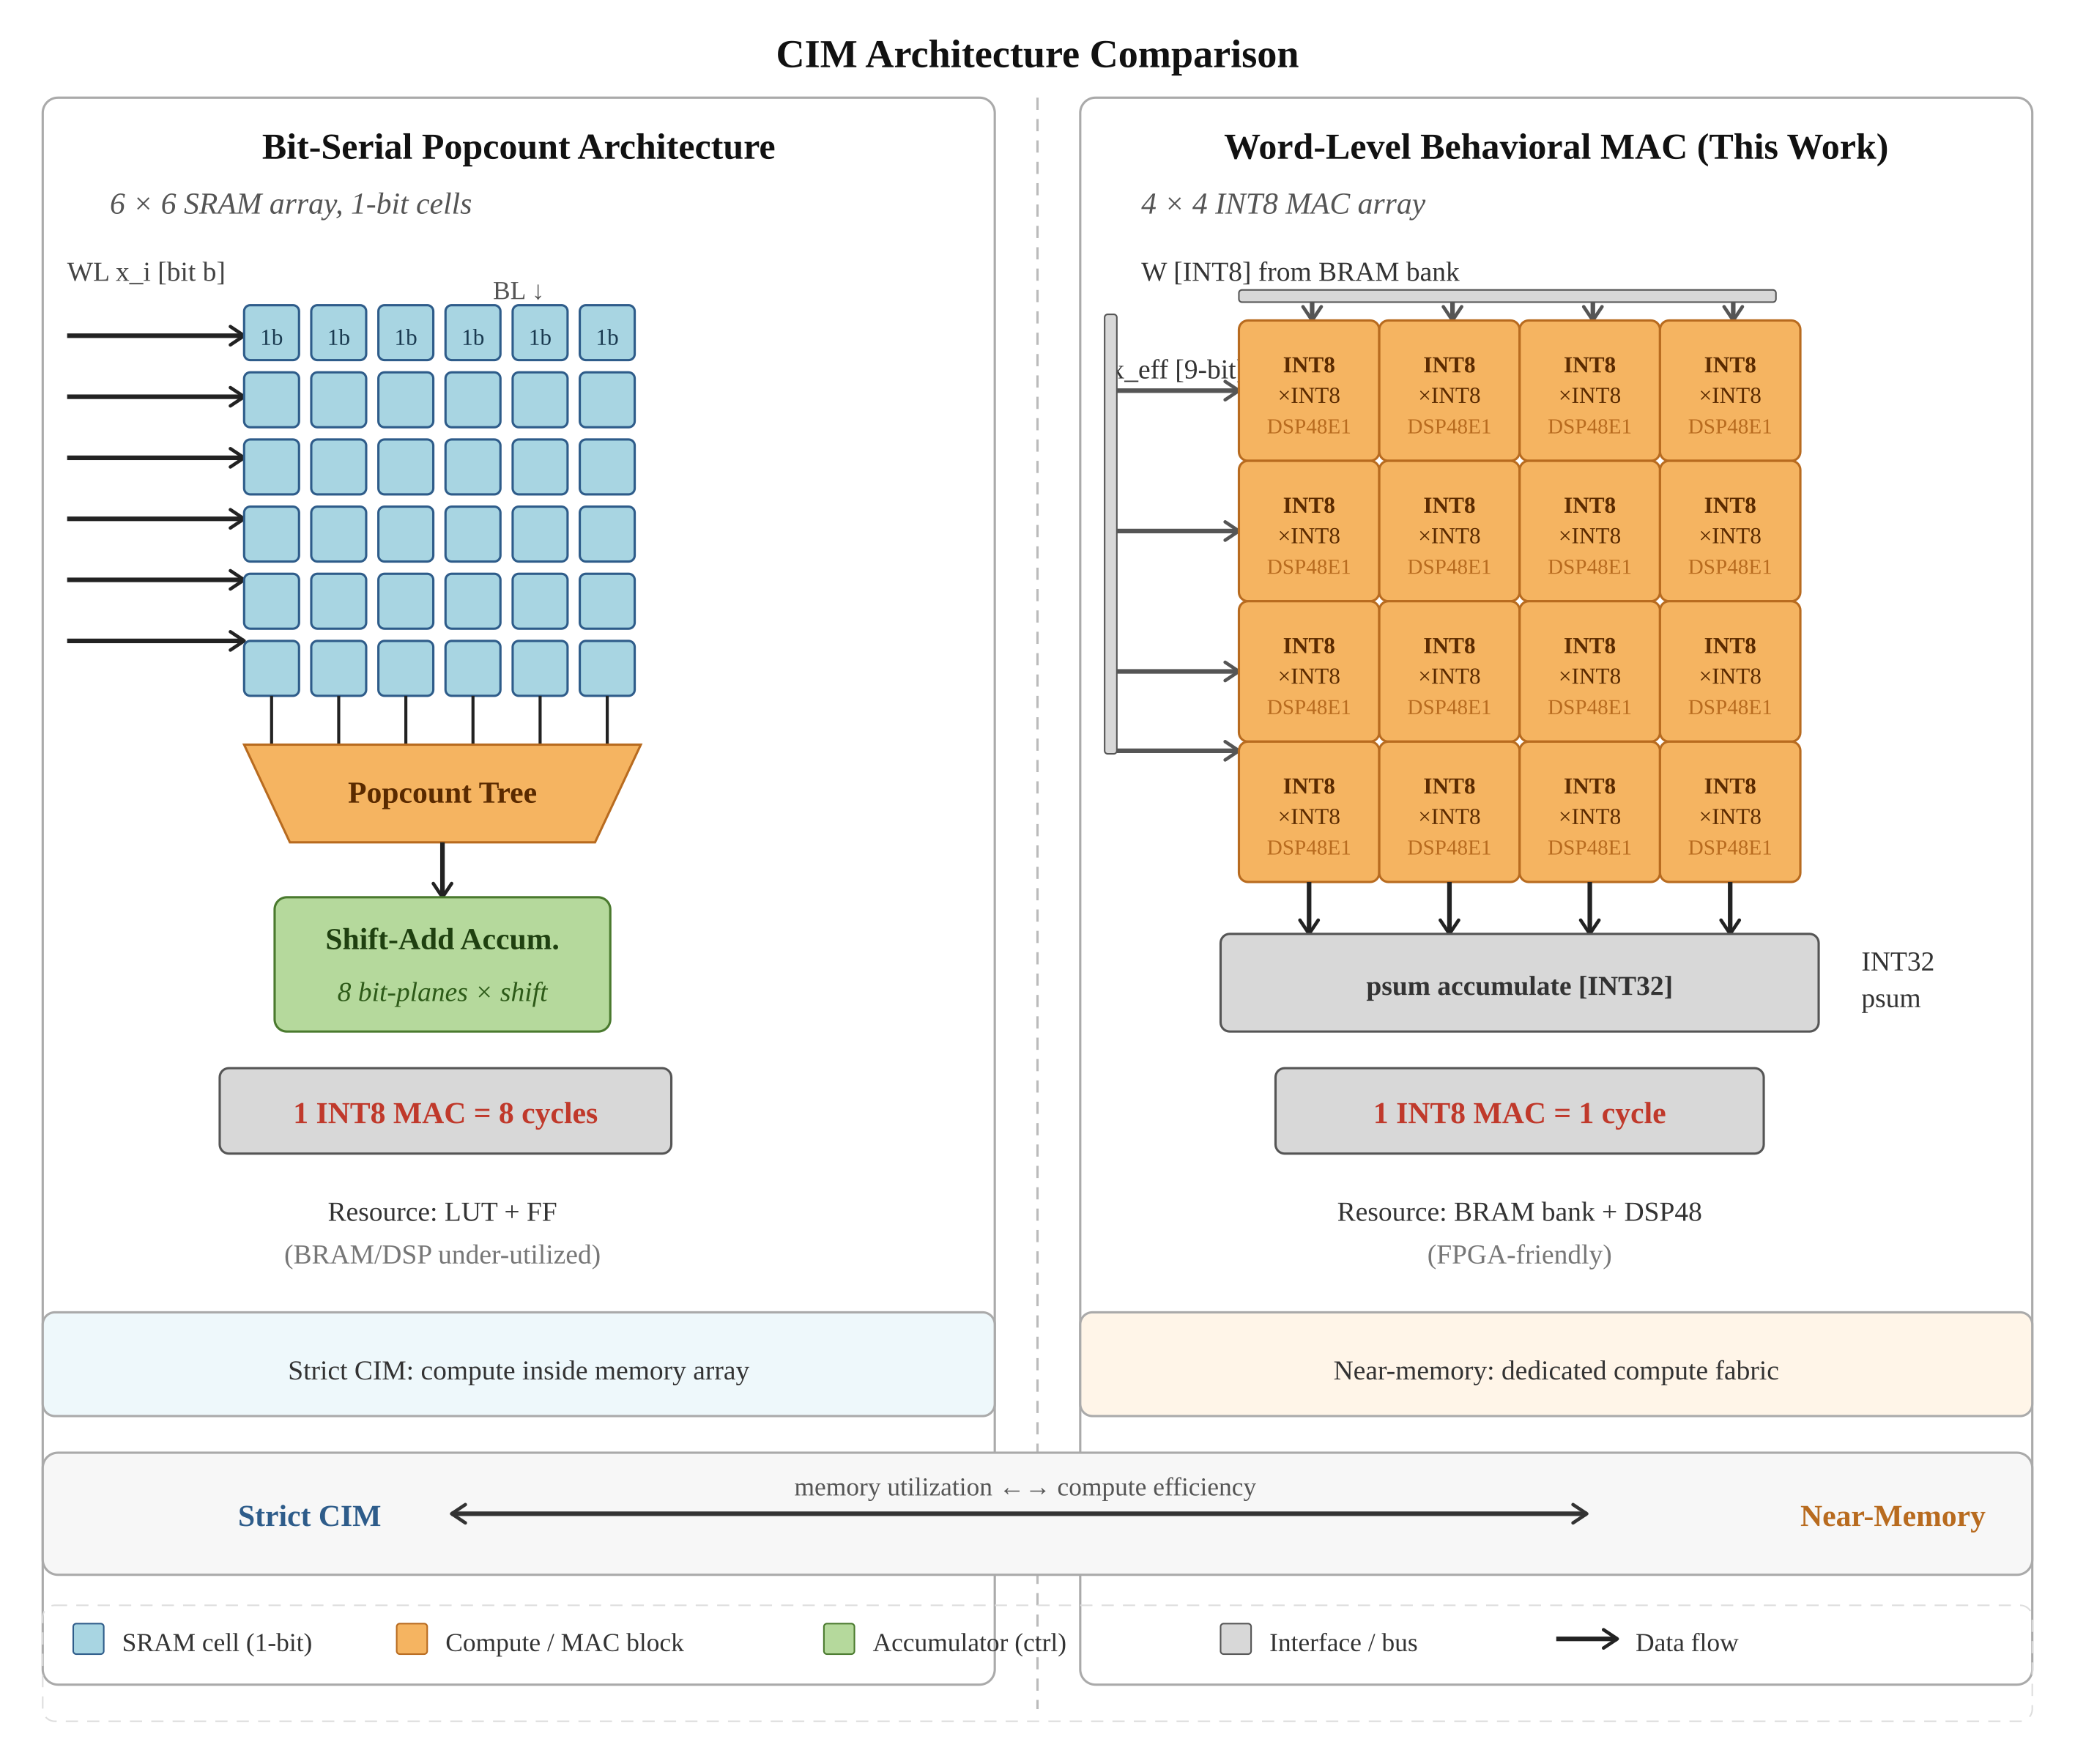
\includegraphics[width=0.95\textwidth]{pics/2-1.png}
	\caption{数字SRAM-CIM两种实现的结构对比。左：比特级bit-serial popcount架构，逼近"存算一体"本义但单MAC需8拍且FPGA不友好；右：字级行为建模MAC架构（本课题），单拍完成MAC、易于映射到DSP48并在FPGA上闭合时序。}
	\label{fig:two_extremes}
\end{figure}

\begin{table}[H]
	\centering
	\caption{数字SRAM-CIM两种实现的对比}
	\label{tab:two_extremes}
	\small
	\begin{tabular}{p{3.0cm}|p{5.0cm}|p{5.0cm}}
		\hline
		\textbf{维度} & \textbf{极端一：bit-serial popcount} & \textbf{极端二：字级行为MAC（本课题）} \\
		\hline
		存储单元粒度 & 1-bit cell，AND+popcount & INT8/INT32字，BRAM \\
		\hline
		INT8 MAC周期数 & 8拍（bit-plane shift-add） & 1拍（组合乘加） \\
		\hline
		阵列规模示例 & $128\times128$ 位 $\times$ 8 bit-plane & $16\times16$ INT8 MAC \\
		\hline
		FPGA资源映射 & LUT+FF为主，BRAM/DSP利用率低 & BRAM bank + DSP48推断 \\
		\hline
		精度后处理位置 & CPU（bias/ReLU/重量化软件完成） & 硬件流水内完成 \\
		\hline
		软件栈复杂度 & 高（需co-sim框架） & 中（Python golden model + 驱动） \\
		\hline
		"存算一体"严格性 & 强（cell即MAC） & 弱（近存储字级MAC） \\
		\hline
		ASIC面积/能效潜力 & 高 & 中 \\
		\hline
		FPGA原型工程性 & 中 & 高 \\
		\hline
		适用场景 & 芯片原型、算法-器件协同 & 工程闭环、系统级演示 \\
		\hline
	\end{tabular}
\end{table}

本课题的目标是\textbf{在PYNQ-Z2这类资源受限的小型FPGA上，搭建一套从量化训练、RTL仿真、FPGA综合到板级推理验证的完整数字CIM闭环}，并将其形态拓展到PicoRV32软核自主控制。本项目重点思考以下内容：（i）硬件能否在目标频率下闭合时序并在PYNQ-Z2上布通；（ii）软硬一致性是否能做到逐层bit-exact可验证；（iii）整体数据通路是否能以单一FSM服务任意层。综合这三点约束，选择字级行为MAC路线是更合理的取舍。因此本章后续的所有模块设计，都围绕"字级INT8 MVM + 硬件化精度后处理 + 单FSM多层复用"这一核心展开。

\subsection{整体架构}

本设计采用"输入缓冲—CIM阵列—累加与量化—输出缓冲"的流水式组织，核心引擎以有限状态机（FSM）驱动完整的推理数据通路。系统顶层架构如图\ref{fig:top_arch}所示：ARM PS（或PicoRV32软核）通过AXI Interconnect以AXI4-Lite配置CSR、以AXI4-Stream（MM2S/S2MM）经AXI DMA与CIM IP批量交换数据；CIM IP内部由接口层（AXI4-Lite Slave、AXIS Sink/Source）、计算层（cim\_accel\_core、cim\_tile、psum\_accum、requant）与存储层（weight\_sram、bias\_sram、input/output\_buffer）三部分构成。系统由以下关键模块组成：
\begin{itemize}
	\item \textbf{cim\_accel\_core}：核心加速器引擎，包含多状态FSM与多级流水线，负责计算调度与性能计数；
	\item \textbf{cim\_tile}：16×16 CIM原子计算单元，纯组合逻辑，实现256个INT8 MAC运算；
	\item \textbf{psum\_accum}：部分和累加器，带优先级清零机制；
	\item \textbf{weight\_sram}：16-bank权重SRAM，支持AXI DMA写入与tile-packed读取；
	\item \textbf{bias\_sram}：偏置SRAM，按输出神经元索引寻址；
	\item \textbf{input\_buffer}：输入缓冲，双bank乒乓结构，支持AXI写入与零点减法；
	\item \textbf{output\_buffer}：输出缓冲，双bank乒乓结构，含argmax逻辑；
	\item \textbf{cim\_axi\_stream\_sink}：AXI4-Stream slave，接收DMA批量数据并路由至各存储模块；
	\item \textbf{cim\_axi\_stream\_source}：AXI4-Stream master，将输出缓冲结果通过DMA批量回传；
	\item \textbf{cim\_axi\_lite\_slave}：AXI4-Lite接口，提供CSR配置、存储窗口访问及stream/legacy路径MUX。
\end{itemize}

\begin{figure}[H]
	\centering
	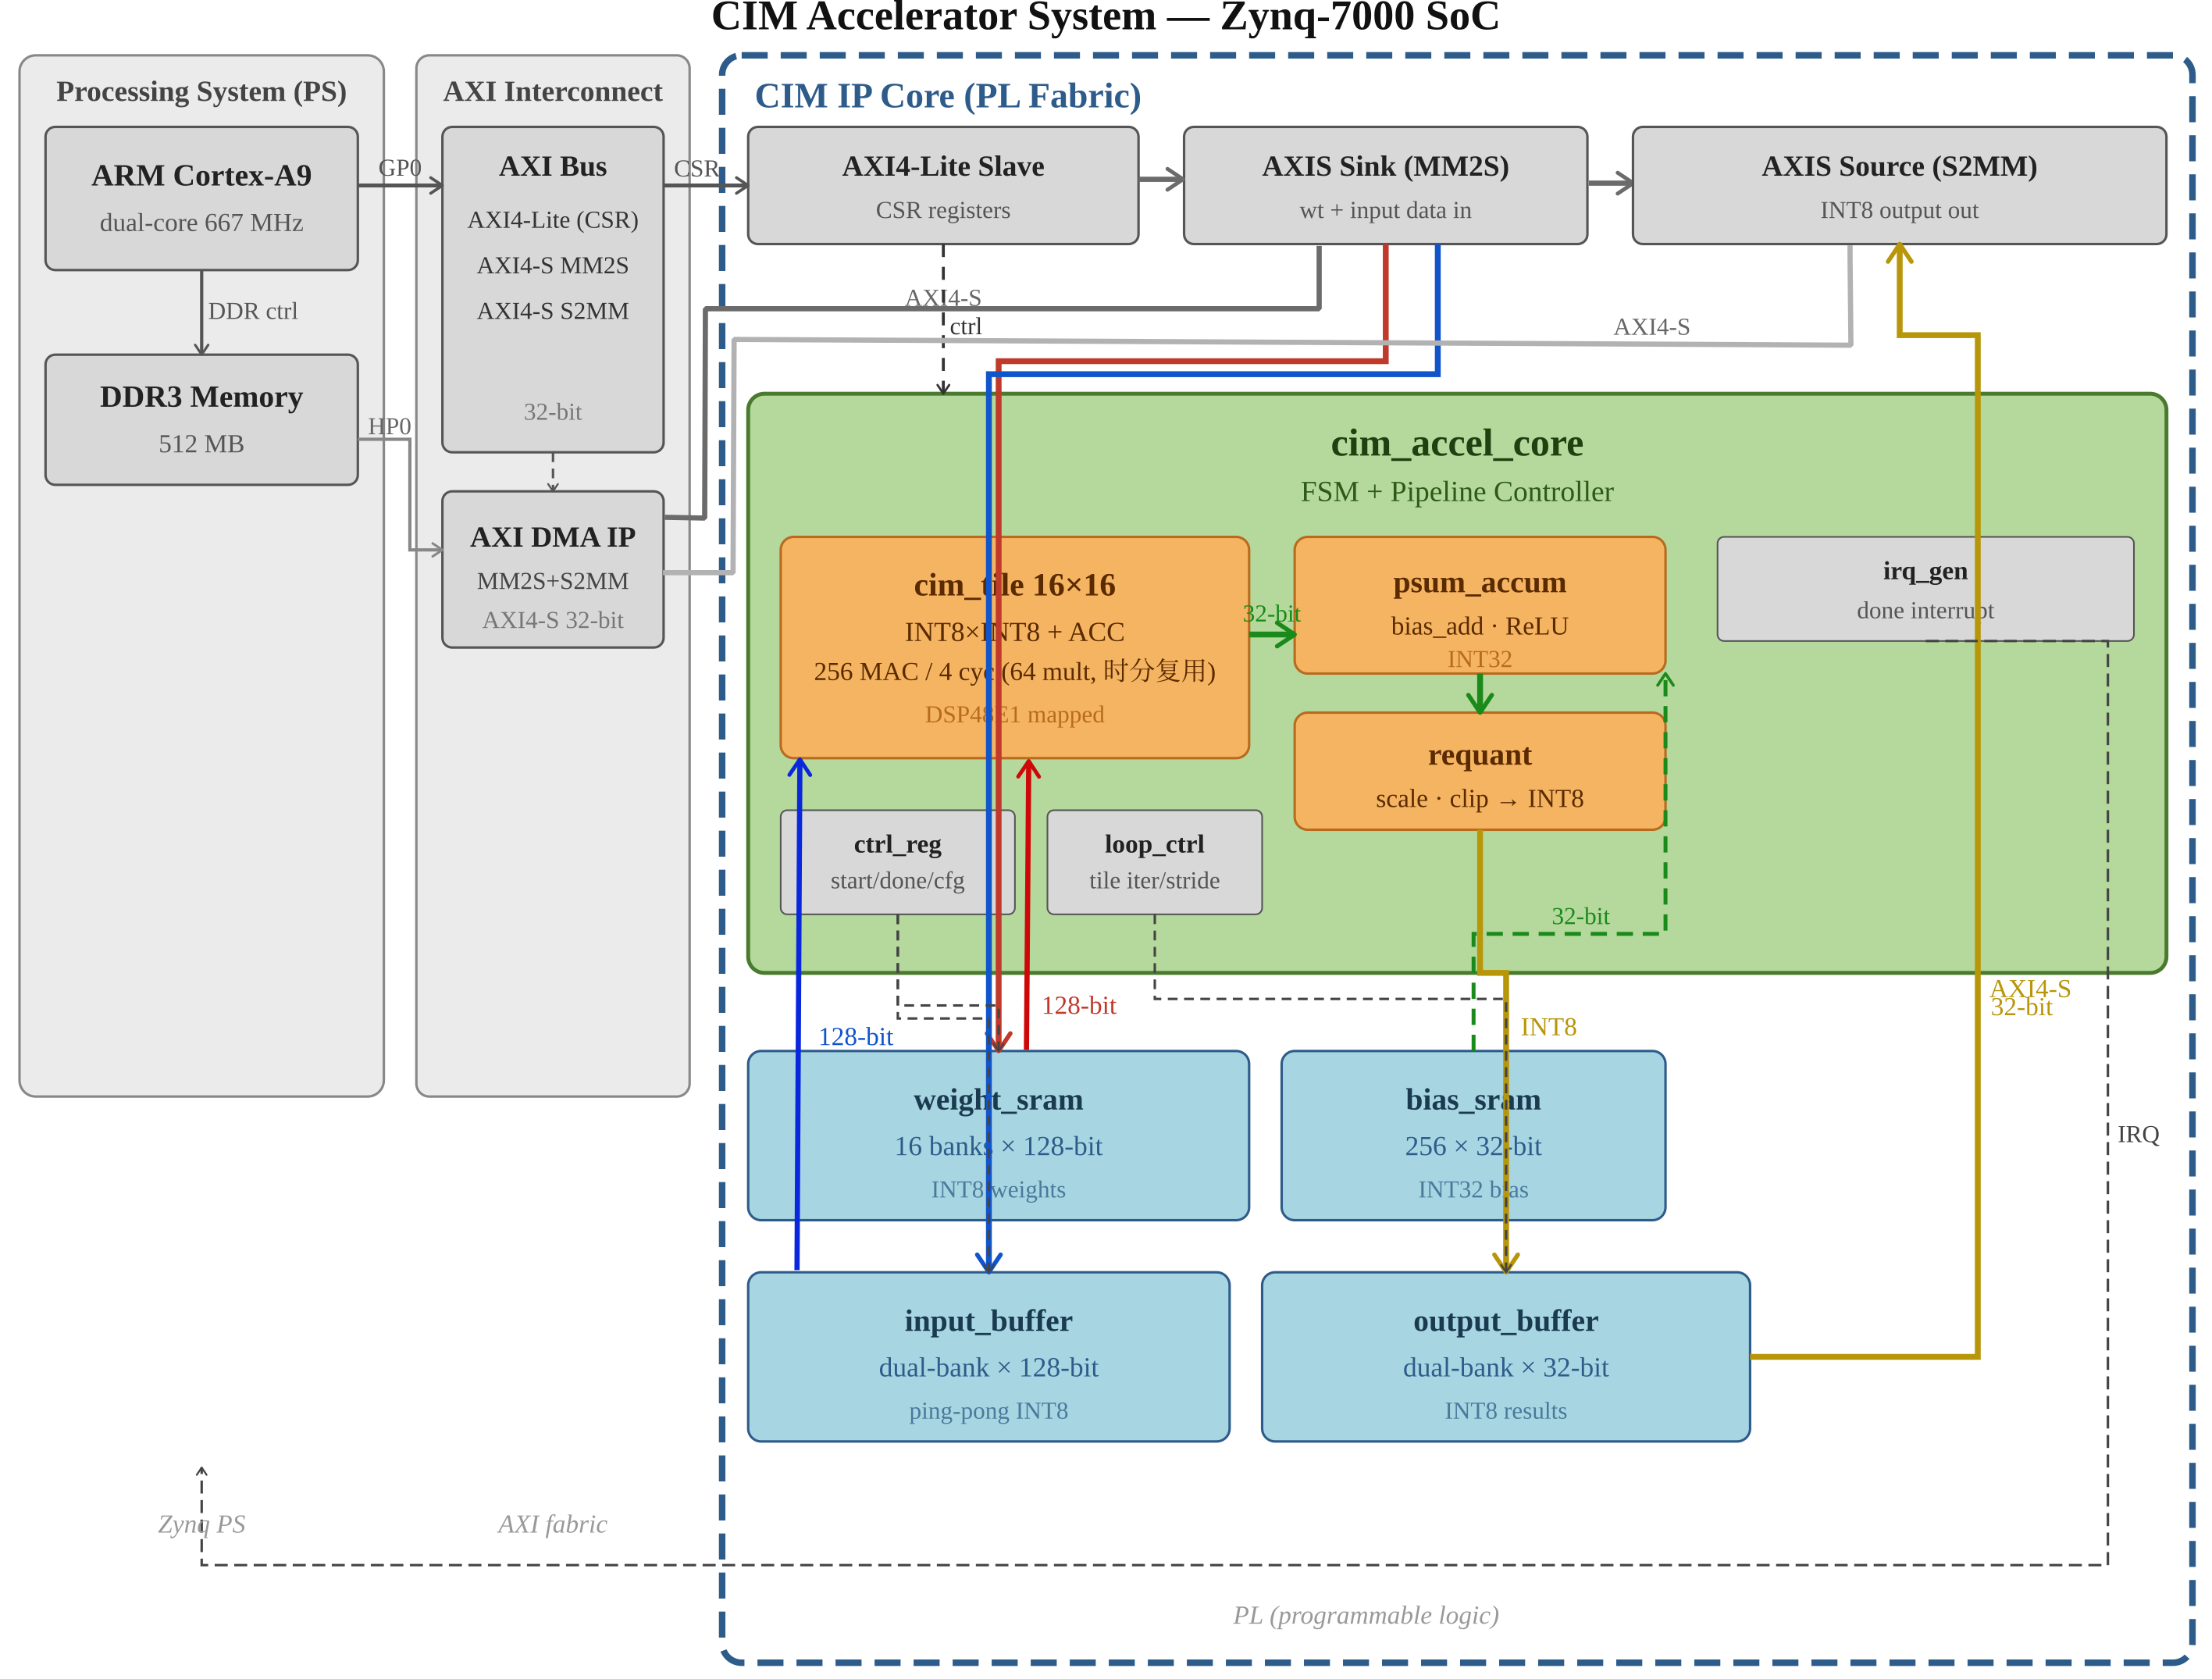
\includegraphics[width=\textwidth]{pics/2-2.png}
	\caption{CIM加速器系统顶层架构框图（Zynq-7000 SoC）。左侧PS通过AXI Interconnect与AXI DMA连接，CIM IP内部分为接口层、计算层（cim\_accel\_core/cim\_tile/psum\_accum/requant）与存储层（权重/偏置SRAM、输入/输出缓冲）。箭头按数据类型着色：权重（红）、输入（蓝）、psum（绿）、INT8结果（黄）。}
	\label{fig:top_arch}
\end{figure}

所有可配置参数集中管理于\texttt{cim\_pkg.sv}文件中，包括Tile尺寸（TILE\_ROWS=16, TILE\_COLS=16）、并行度（PAR\_OB）、MAC拆分因子（TILE\_SPLIT\_FACTOR）、数据位宽（INT8输入/权重、INT32偏置/累加器）、最大层维度（MAX\_IN\_DIM=1536, MAX\_OUT\_DIM=256）、CSR地址映射与FSM状态编码。保证项目不存在magic number，所有RTL模块通过\texttt{import cim\_pkg::*}引用参数。

加速器的工作流程为：PS（或PicoRV32）通过AXI4-Stream DMA接口批量写入权重、偏置与输入数据，通过AXI4-Lite接口配置层参数（IN\_DIM, OUT\_DIM, N\_IB, N\_OB, requant\_mult, requant\_shift, act\_mode, input\_zp），然后触发start信号。核心引擎按output-block并行、input-block迭代的顺序完成MVM运算，每轮计算后进行偏置累加、激活与重量化，最终将INT8结果写入输出缓冲。完成后置位done信号并可触发IRQ。对于连续FC层，层融合机制可将OBUF结果通过内部硬件路径直接拷贝至IBUF，避免DMA往返。

\subsection{CIM Tile设计}

CIM Tile是本设计的原子计算单元，实现以下运算：

\begin{equation}
	\text{psum}[r] = \sum_{c=0}^{15} \text{x\_eff}[c] \times w[r][c], \quad r = 0, 1, \ldots, 15
\end{equation}

其中$\text{x\_eff}$为经过零点减法后的9位无符号有效输入，$w$为Signed-INT8权重，输出为32位有符号部分和。原始UINT8像素值$[0,255]$减去零点$\text{input\_zp}=-128$（即加上128），得到范围为$[128,383]$的9位无符号值。

Tile采用纯组合逻辑实现，通过generate构造16行×16列的乘加阵列。每行独立计算一个输出神经元的部分和，列方向采用链式累加：

\begin{equation}
	\text{row\_acc}[c+1] = \text{row\_acc}[c] + \text{signed\_extend}(\text{x\_eff}[c]) \times w[r][c]
\end{equation}

每个Tile每个时钟周期产生$16 \times 16 = 256$个MAC运算的结果。采用纯组合设计的原因是将时序控制集中在核心引擎的FSM中，Tile本身作为"存储阵列做计算"的数字抽象。其内部结构如图\ref{fig:cim_tile}所示：有效输入$\text{x\_eff}$沿行方向广播，权重沿列方向由对应bank送入，每行通过链式累加得到一个INT32部分和，一拍输出16个$\text{psum}$。

\begin{figure}[H]
	\centering
	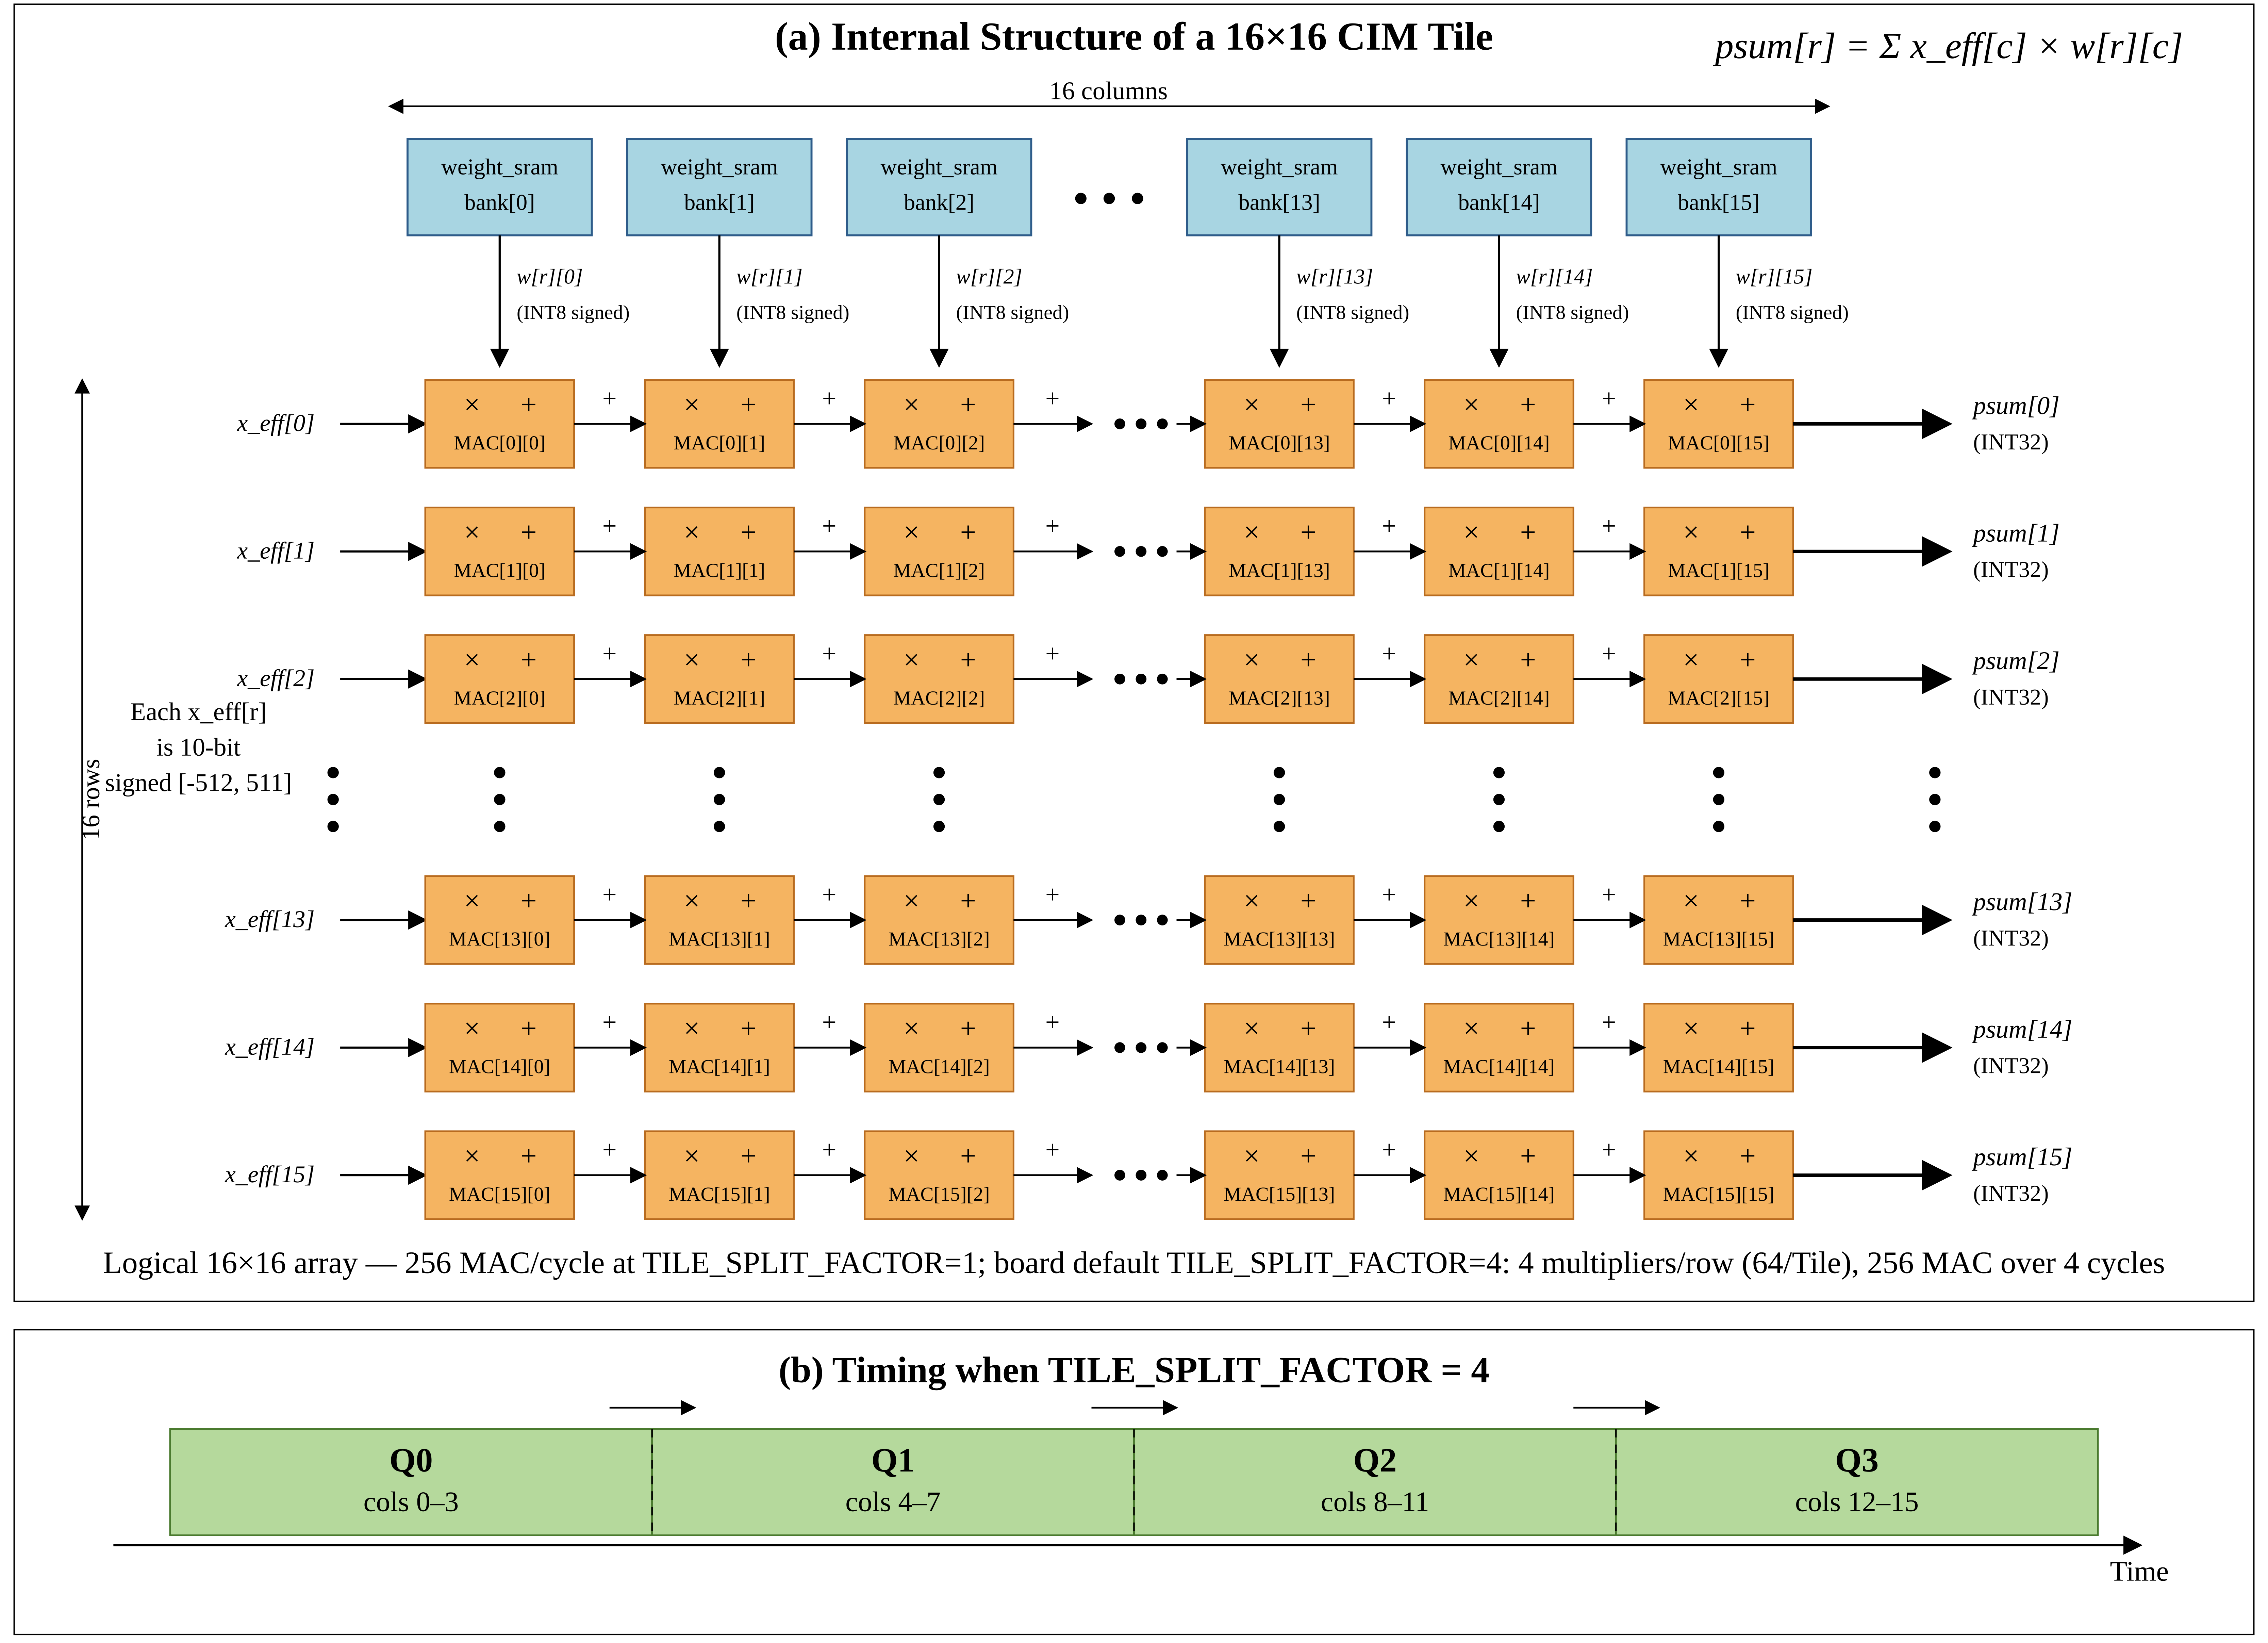
\includegraphics[width=0.92\textwidth]{pics/2-3.png}
	\caption{16$\times$16 CIM Tile内部结构。9位有效输入$\text{x\_eff}$沿行广播，Signed-INT8权重沿列输入，列方向链式累加得到16个INT32部分和；下方子图为TILE\_SPLIT\_FACTOR=4时Q0$\sim$Q3四拍时序拆分。}
	\label{fig:cim_tile}
\end{figure}


为支持更高时钟频率，Tile内部的16列MAC可通过编译期参数\texttt{TILE\_SPLIT\_FACTOR}拆分为多组顺序执行。当\texttt{TILE\_SPLIT\_FACTOR}=4时，16列被分为4组（每4列一组），分4个时钟周期计算：

\begin{equation}
	\text{psum}[r] = \sum_{q=0}^{3} \sum_{c=4q}^{4q+3} \text{x\_eff}[c] \times w[r][c], \quad r = 0, \ldots, 15
\end{equation}

每组仅含4个MAC + 单个CARRY4进位链，组合路径从约16 ns降至约5 ns，从而实现100 MHz的工作频率。FSM相应地从单一ST\_MAC状态扩充为ST\_MAC\_Q0→Q1→Q2→Q3四拍顺序执行，每IB迭代增加3个额外周期。这一拆分策略的代价是MAC吞吐率下降（4拍完成原1拍的工作），但其价值在于为非MAC流水级（bias/ReLU/重量化）提供更高的时钟频率，并为双缓冲乒乓重叠提供时序裕量。

\subsection{存储子系统}

\subsubsection{权重SRAM的BRAM推断问题与bank拆分方案}

权重SRAM的设计是本项目的关键工程挑战之一。初始设计中，weight SRAM为一整块2048位宽（$\text{TILE\_ROWS} \times \text{TILE\_COLS} \times 8 = 2048$位）的存储器。然而，Vivado对这种超宽memory推断BRAM本身就困难；更关键的是，如果用bit-select方式做32位chunk部分写入，Vivado会直接放弃BRAM推断，退化为纯寄存器，导致资源爆炸。

解决方案是将weight SRAM拆分为16个独立的bank，每个bank仅$\text{ROW\_W} = \text{TILE\_COLS} \times \text{WEIGHT\_W} = 128$位宽，对应Tile的一行权重。16个bank通过generate实例化，每个bank独立推断为BRAM：

\begin{equation}
	\text{bank\_mem}[r][\text{tile\_idx}] = \{w[r][15], w[r][14], \ldots, w[r][0]\}, \quad r = 0, \ldots, 15
\end{equation}

写入侧使用staging register将4个32位AXI写入累积为完整的128位行数据，然后通过单周期整字写入送入对应bank，确保了BRAM推断所需的"纯整字写入"条件。该bank拆分前后的对比如图\ref{fig:weight_bank}所示。

\begin{figure}[H]
	\centering
	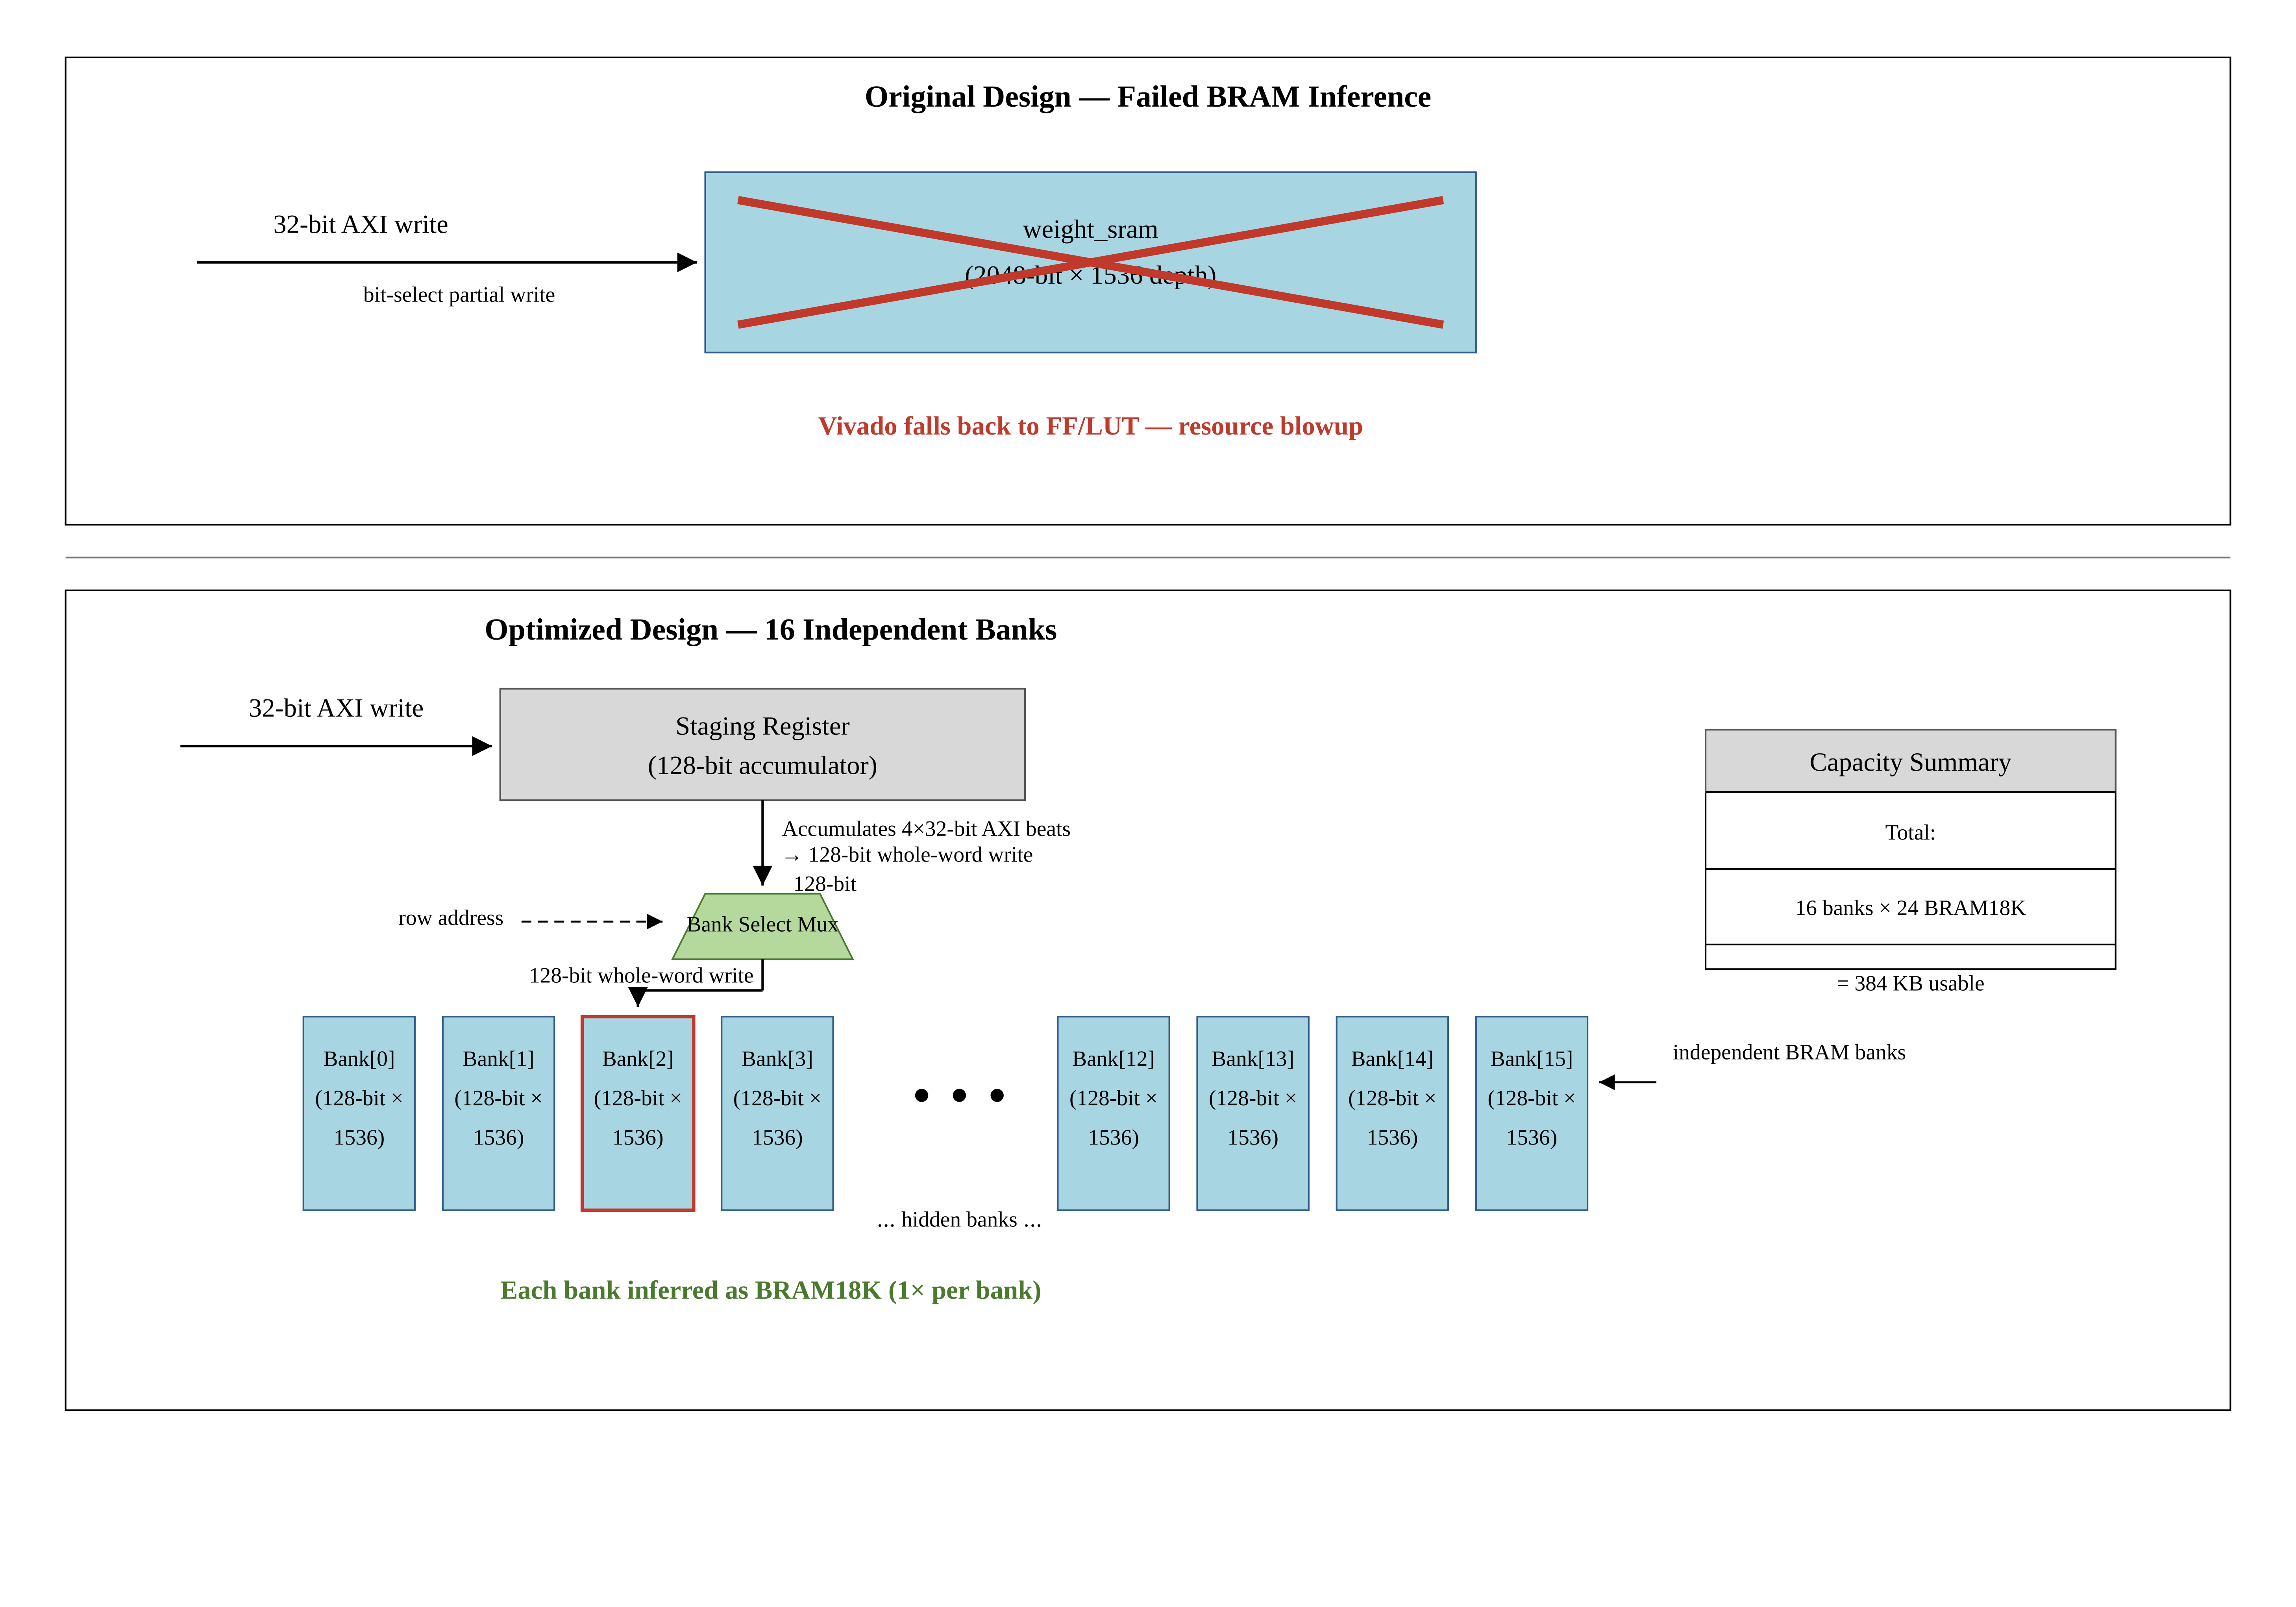
\includegraphics[width=0.9\textwidth]{pics/2-4.png}
	\caption{权重SRAM的16-bank拆分方案对比。上：原始2048位单块在32位部分写入下无法被Vivado推断为BRAM，退化为FF/LUT；下：拆分为16个独立128位bank，配合staging register将4个32位AXI beat组装为128位整行写入，每个bank均成功推断为BRAM。}
	\label{fig:weight_bank}
\end{figure}


\begin{table}[H]
	\centering
	\caption{权重SRAM设计参数}
	\begin{tabular}{lcc}
		\toprule
		参数 & 值 & 说明 \\
		\midrule
		Bank数量 & 16 & 对应TILE\_ROWS \\
		Bank宽度 & 128 bits & TILE\_COLS $\times$ WEIGHT\_W \\
		Bank深度 & 1536 & 扩展后的最大tile容量 \\
		总容量 & 393,216 bytes & $16 \times 128 \times 1536 / 8$ \\
		写入接口 & 128-bit whole-word & 确保BRAM推断 \\
		读取延迟 & 1 cycle & registered read \\
		\bottomrule
	\end{tabular}
\end{table}

\subsubsection{偏置SRAM与输入/输出缓冲}

偏置SRAM按输出神经元索引寻址，每个条目32位（INT32），深度为MAX\_OUT\_DIM=256。输入缓冲存储tile-packed的输入数据，每条目$\text{TILE\_COLS} \times \text{INPUT\_W} = 128$位。输入缓冲在读取时自动完成零点减法：

\begin{equation}
	\text{x\_eff}[c] = \text{input}[c] - \text{input\_zp}
\end{equation}

其中input\_zp通过CSR配置，默认为$-128$（相当于将UINT8像素值整体上移128，确保x\_eff为非负的9位无符号值，范围$[128,383]$）。输出缓冲存储INT8推理结果，并内置argmax比较逻辑，在末层推理完成后自动给出预测类别。

\subsubsection{IBUF/OBUF双缓冲乒乓设计}

为将DMA数据传输与CIM计算重叠执行，输入缓冲和输出缓冲各自实现了双bank（bank0/bank1）乒乓结构。设计原则为最小化核心改动：\texttt{cim\_accel\_core.sv}完全不感知bank的存在，bank选择逻辑完全封装在\texttt{cim\_axi\_lite\_slave.sv}中，通过单个CSR位\texttt{CSR\_PING\_CTRL}（地址0x06C）控制，写1翻转（toggle）、写0为no-op。

Bank选择规则如表\ref{tab:pingpong_bank}所示：CIM compute始终使用\texttt{reg\_ping\_ctrl}选中的"活跃bank"（读IBUF活跃bank、写OBUF活跃bank），而DMA始终访问其反码对应的"非活跃bank"（写IBUF非活跃bank、读OBUF非活跃bank）。一次toggle操作即可原子性地交换DMA与compute的访问目标，实现DMA传输与硬件计算的无冲突重叠。

\begin{table}[H]
	\centering
	\caption{双缓冲Bank选择逻辑}
	\label{tab:pingpong_bank}
	\begin{tabular}{lcl}
		\toprule
		信号 & 公式 & 用途 \\
		\midrule
		ibuf rd bank & \texttt{reg\_ping\_ctrl} & Compute从活跃bank读取输入 \\
		obuf wr bank & \texttt{reg\_ping\_ctrl} & Compute向活跃bank写入结果 \\
		ibuf wr bank & \texttt{\~reg\_ping\_ctrl} & DMA向非活跃bank写入下一批输入 \\
		obuf rd bank & \texttt{\~reg\_ping\_ctrl} & DMA从非活跃bank读回上一批结果 \\
		\bottomrule
	\end{tabular}
\end{table}

Python驱动侧有\texttt{toggle\_bank()}、\texttt{start\_compute()}（非阻塞触发）与\texttt{wait\_for\_done()}（阻塞轮询）三个原语。核心编排逻辑的乒乓序列如图\ref{fig:pingpong}所示，分为cold start、overlap与tail三个阶段：cold start阶段加载首批输入→翻转bank→启动计算；overlap循环阶段在compute(i-1)进行的同时通过DMA向非活跃bank加载input(i)，compute完成后翻转bank并立即启动下一轮计算，同时从非活跃bank读回上一轮结果；tail阶段处理最后一批结果的读回。对于Conv层的批量推理，将所有图像的$k_{\text{pack}}$批次收集为单一列表，一次乒乓调用完成整个卷积层的全部MVM推理，最大化重叠批次数。

\begin{figure}[H]
	\centering
	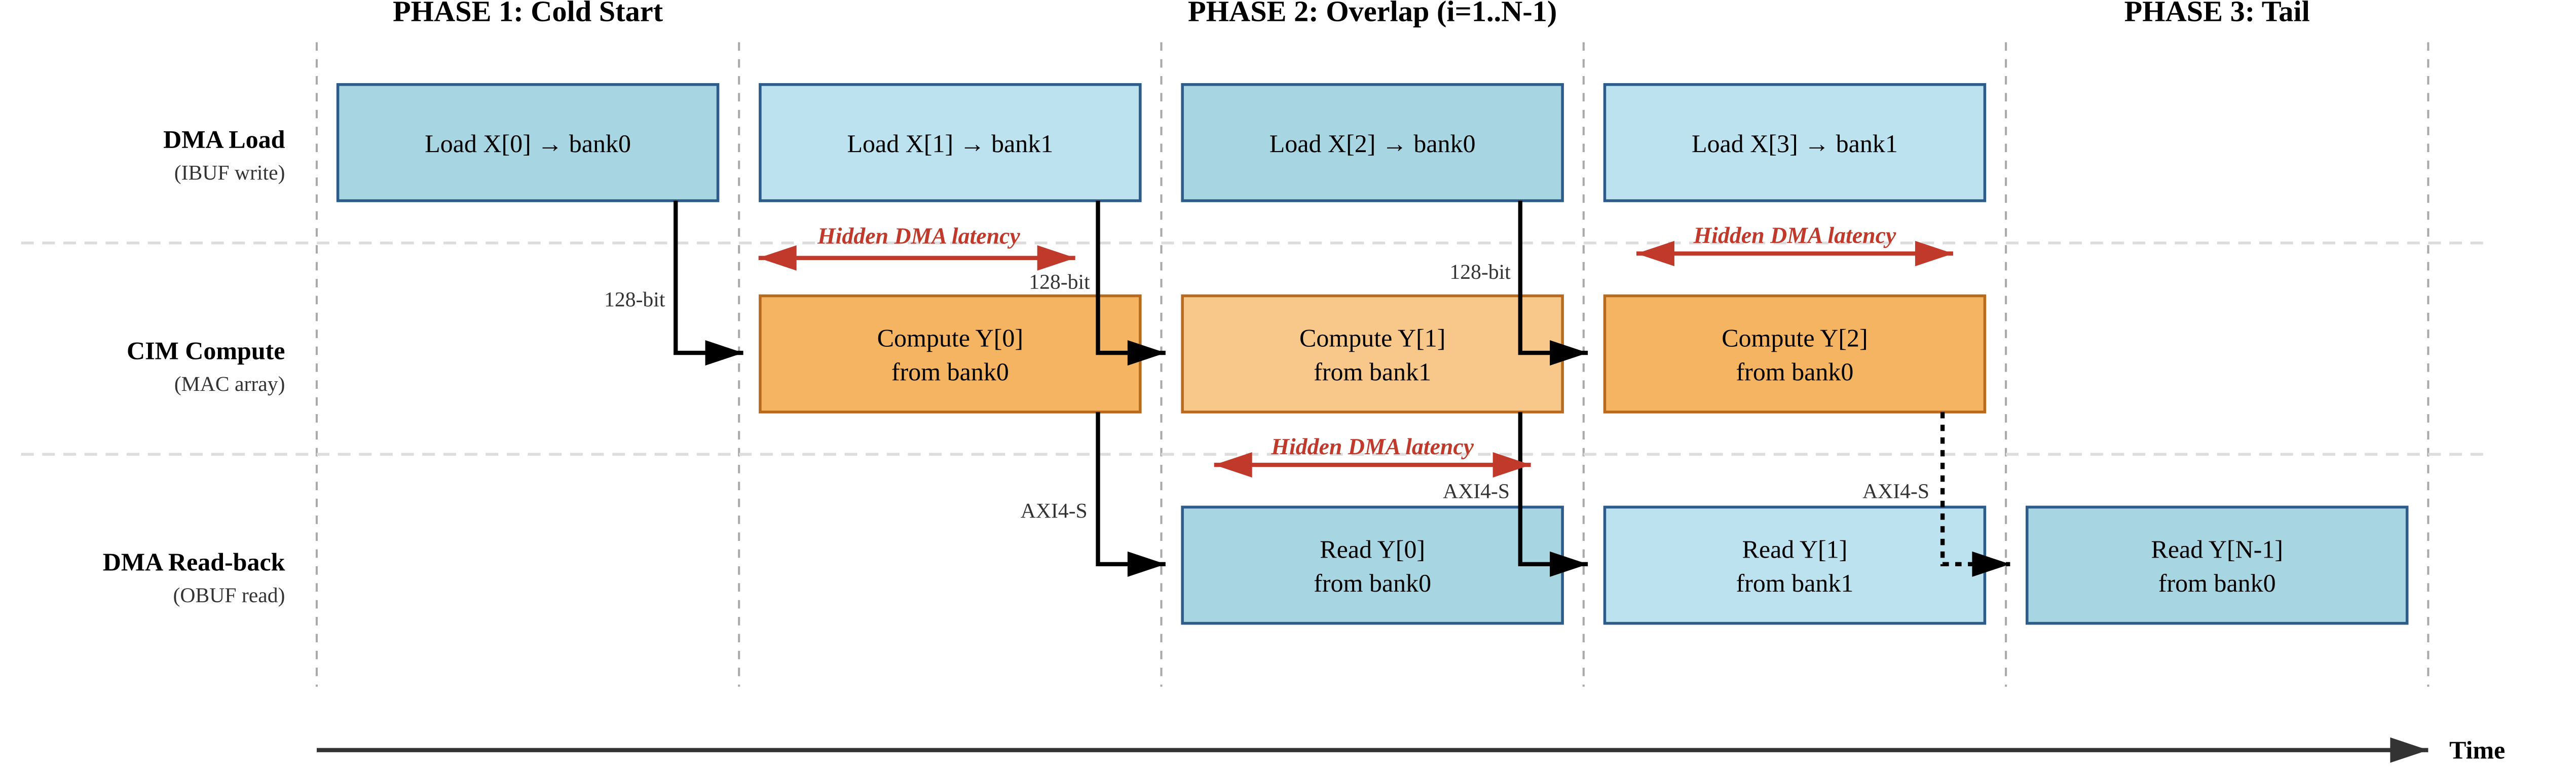
\includegraphics[width=\textwidth]{pics/2-5.png}
	\caption{IBUF/OBUF双缓冲乒乓执行时序图。DMA load、CIM compute与DMA read-back三条泳道共享时间轴；overlap阶段DMA传输被隐藏在计算之后（阴影区），一次\texttt{toggle}操作原子性地交换DMA与compute的bank分配。}
	\label{fig:pingpong}
\end{figure}

\subsection{量化与重定标}

本设计的量化流程遵循标准INT8整数推理规范\cite{6}，确保与软件golden model的bit-exact一致性。完整的量化链路为：

\begin{equation}
	\text{psum} = \sum_c \text{x\_eff}[c] \times w[r][c] + \text{bias}[r]
\end{equation}

\begin{equation}
	\text{prod} = \text{psum} \times \text{requant\_mult}
\end{equation}

\begin{equation}
	\text{shifted} = \left\lfloor \frac{\text{prod} + 2^{\text{requant\_shift}-1}}{2^{\text{requant\_shift}}} \right\rfloor
\end{equation}

\begin{equation}
	\text{output} = \text{clamp}(\text{shifted}, -128, 127)
\end{equation}

其中requant\_mult和requant\_shift为每层可配置的量化参数，通过CSR在运行时设置。重定标过程中使用64位中间乘积以避免溢出，移位时采用带舍入的算术右移（round-half-up），最后clamp到INT8范围$[-128, 127]$。

激活函数支持三种模式：无激活（ACT\_NONE）、ReLU（ACT\_RELU，将负值归零）、范围截断（ACT\_CLAMP）。模式通过CSR的ACT\_MODE寄存器配置。完整的量化重定标数据通路及各级位宽与对应FSM状态如图\ref{fig:requant}所示。

\begin{figure}[H]
	\centering
	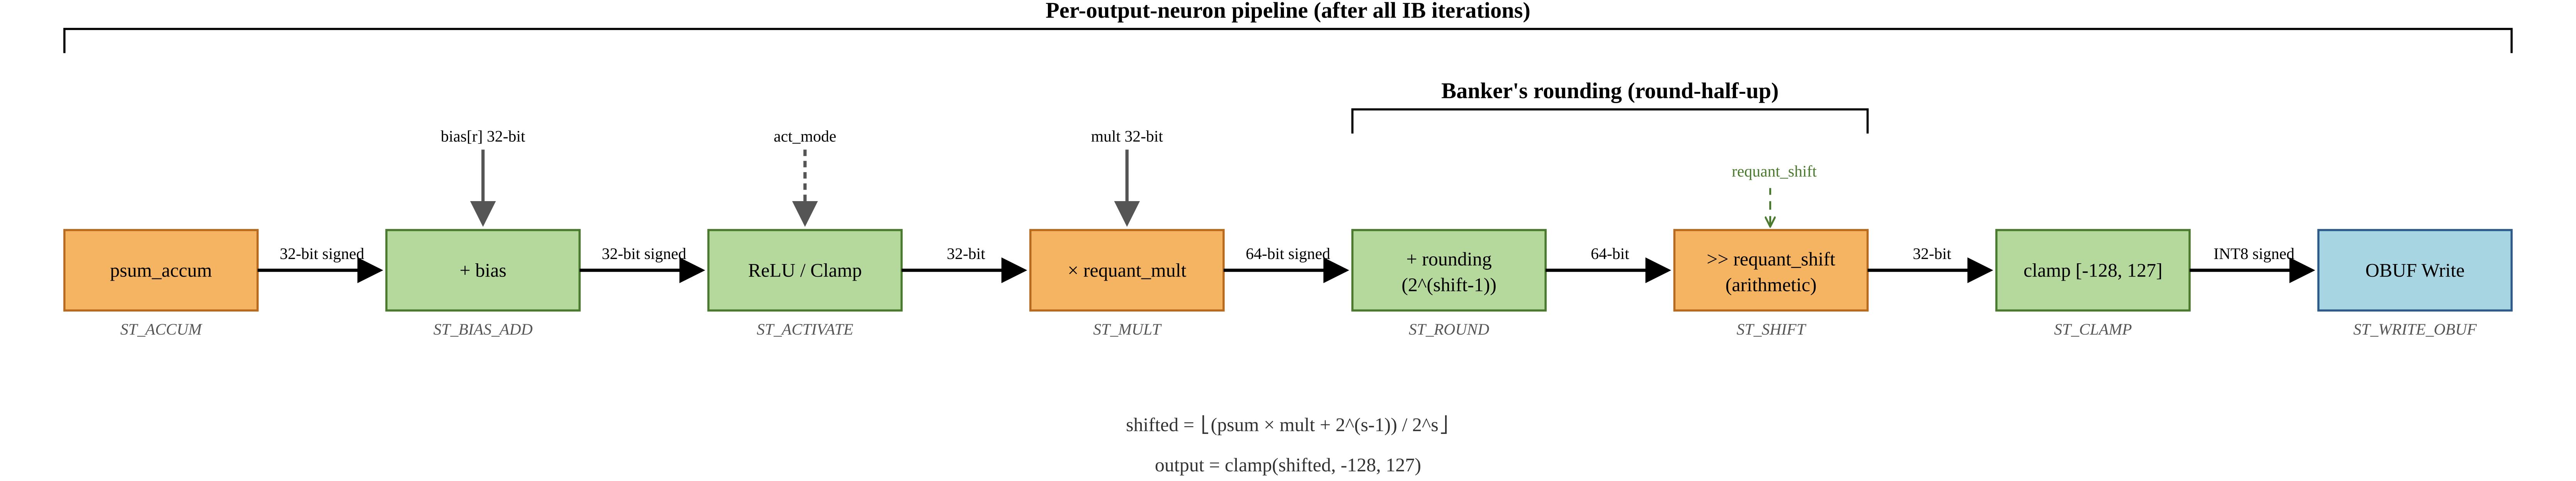
\includegraphics[width=\textwidth]{pics/2-6.png}
	\caption{量化重定标数据通路流水线。从psum累加经加偏置、ReLU/clamp、乘requant\_mult（升至64位）、加舍入项、算术右移、clamp至INT8，逐级标注位宽（32$\to$32$\to$32$\to$64$\to$64$\to$32$\to$8）与对应FSM状态。}
	\label{fig:requant}
\end{figure}

\subsection{AXI4-Stream DMA数据通路}

系统通过AXI4-Stream + Xilinx axi\_dma IP实现双向批量数据传输，替代传统AXI4-Lite逐字MMIO。


\subsubsection{MM2S写入通路}

权重、输入与偏置的加载走DDR→\allowbreak S\_AXI\_HP0→\allowbreak axi\_dma→\allowbreak M\_AXIS\_MM2S→\allowbreak cim\_axi\_stream\_sink的批量stream路径。\texttt{cim\_axi\_stream\_sink}内部实现4-beat到128-bit行装配：每4个32-bit AXI4-Stream beat组成一个完整的128-bit行写入，根据CSR配置的dest字段（0=weight, 1=input, 2=bias）路由至对应存储模块。CSR控制仍保留原AXI4-Lite接口，CIM计算核心（\texttt{cim\_tile}、\texttt{psum\_accum}、\texttt{cim\_accel\_core}）完全不动。

关键设计决策包括：（1）AXIS数据宽度=32-bit，与现有weight\_to\_chunks软件packing兼容，DMA内部利用Data Realignment Engine做64→32免费dwidth转换；（2）dual-path共存——在\texttt{cim\_axi\_lite\_slave}内部通过CSR\_CTRL[3]对写入路径做MUX，legacy MMIO路径保留用于A/B对照与回归隔离；（3）cfg\_start通过写CSR\_STREAM\_LEN隐式触发，原子化操作省去额外的CSR写开销；（4）s\_axis\_tready恒为1——BRAM写为单周期完成，sink内部无需排队，反压沿由DMA侧向PS端反向传播。该sink将4个32位beat装配为128位行并按dest字段路由的过程如图\ref{fig:axis_sink}所示。

\begin{figure}[H]
	\centering
	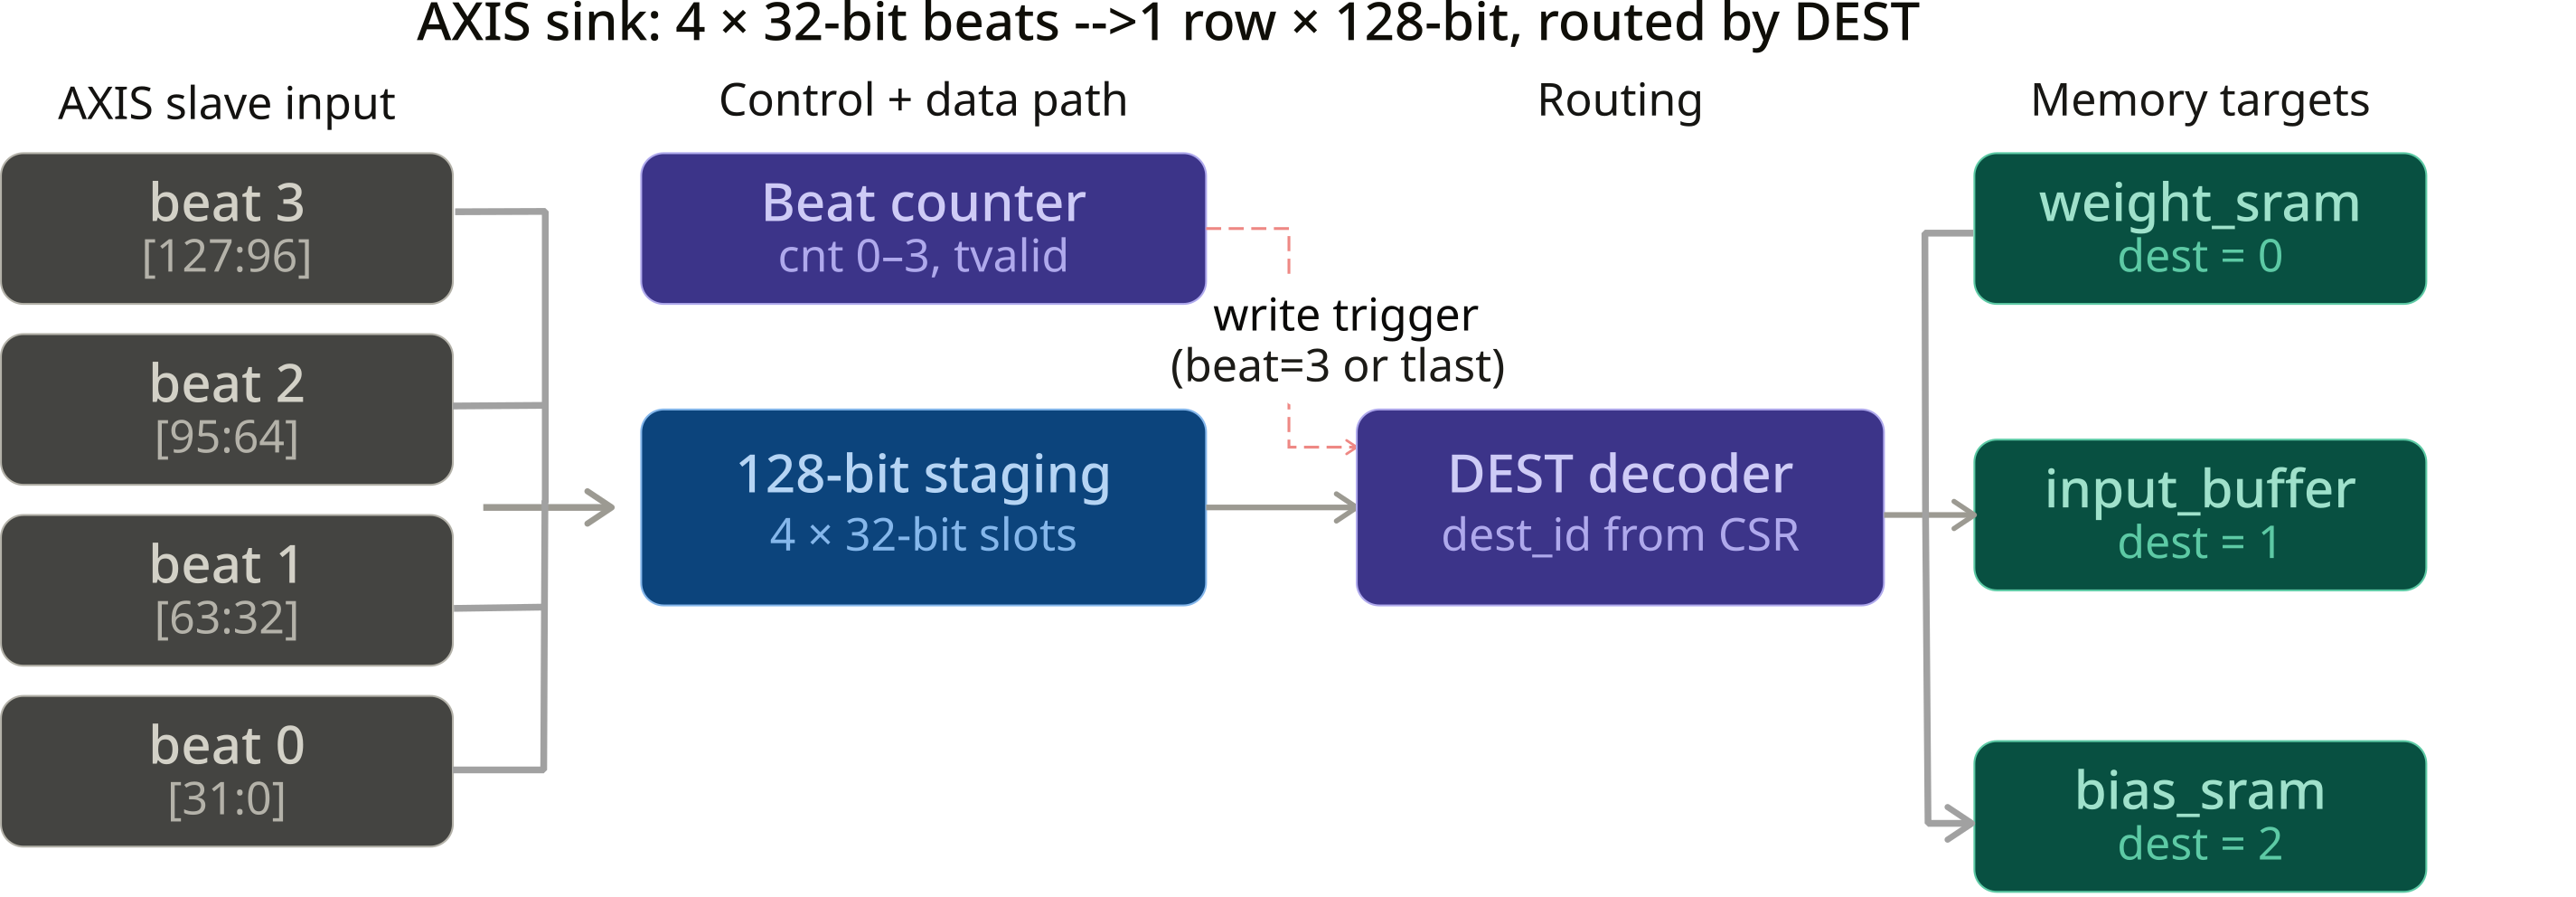
\includegraphics[width=0.92\textwidth]{pics/2-7.png}
	\caption{cim\_axi\_stream\_sink的4-beat到128-bit行装配示意图。4个32位AXIS beat按字段位置写入128位staging register，整字写入后由DEST译码器根据dest\_id路由至权重SRAM、输入缓冲或偏置SRAM。}
	\label{fig:axis_sink}
\end{figure}

\subsubsection{S2MM读回通路}

推理结果的读回走output\_buffer→\allowbreak cim\_axi\_stream\_source→\allowbreak M\_AXIS\_RESULT→\allowbreak axi\_dma/S\_AXIS\_S2MM→\allowbreak S\_AXI\_HP1→\allowbreak DDR的批量stream路径。\texttt{cim\_axi\_stream\_source}采用5状态FSM（IDLE→WAIT→WARMUP→READ→SEND）处理BRAM的2-cycle读延迟与非4对齐末字打包。每4个INT8结果打包为一个32-bit AXI4-Stream beat，末拍置tlast=1告知DMA结束接收。Python驱动侧采用direct register mode直接操作S2MM的DMACR/DA/LENGTH寄存器，并实现双缓冲交替机制避免缓冲区复用问题。

\subsection{Layer Fusion：OBUF→IBUF内部硬件直拷}

针对连续全连接层（如LeNet-5的FC3→FC4→FC5或MLP的FC1→FC2），标准数据流需要在层间执行完整的S2MM读回→DDR→MM2S重新加载循环。本设计在\texttt{cim\_axi\_lite\_slave}中实现了OBUF→IBUF内部硬件拷贝的层融合（Layer Fusion）机制。

融合FSM包含4个状态（F\_IDLE→F\_WAIT\_MUX→F\_PACK→F\_WRITE），工作流程为：OBUF按字节读取INT8结果→在硬件内部重新打包为128-bit tile字（16 INT8/tile）→直接写入IBUF。通过F\_WAIT\_MUX状态处理OBUF读路径的流水线延迟（always\_comb MUX传播 + BRAM registered read共2周期），确保byte-to-tile装配的字节对齐正确性。

约束条件为融合元素数$n\_elements \leq \text{MAX\_OUT\_DIM} = 256$，单次融合耗时$n\_elements + 1 + \lceil n\_elements/16 \rceil \times 2$周期。以FC1→FC2（128元素）为例，融合延迟约1.5 $\mu$s，远小于等效的DMA S2MM+MM2S往返延迟（数十毫秒）。图\ref{fig:layer_fusion}（a）对比了有无层融合两种数据流的层间延迟，（b）给出了融合FSM的状态转移。

\begin{figure}[H]
	\centering
	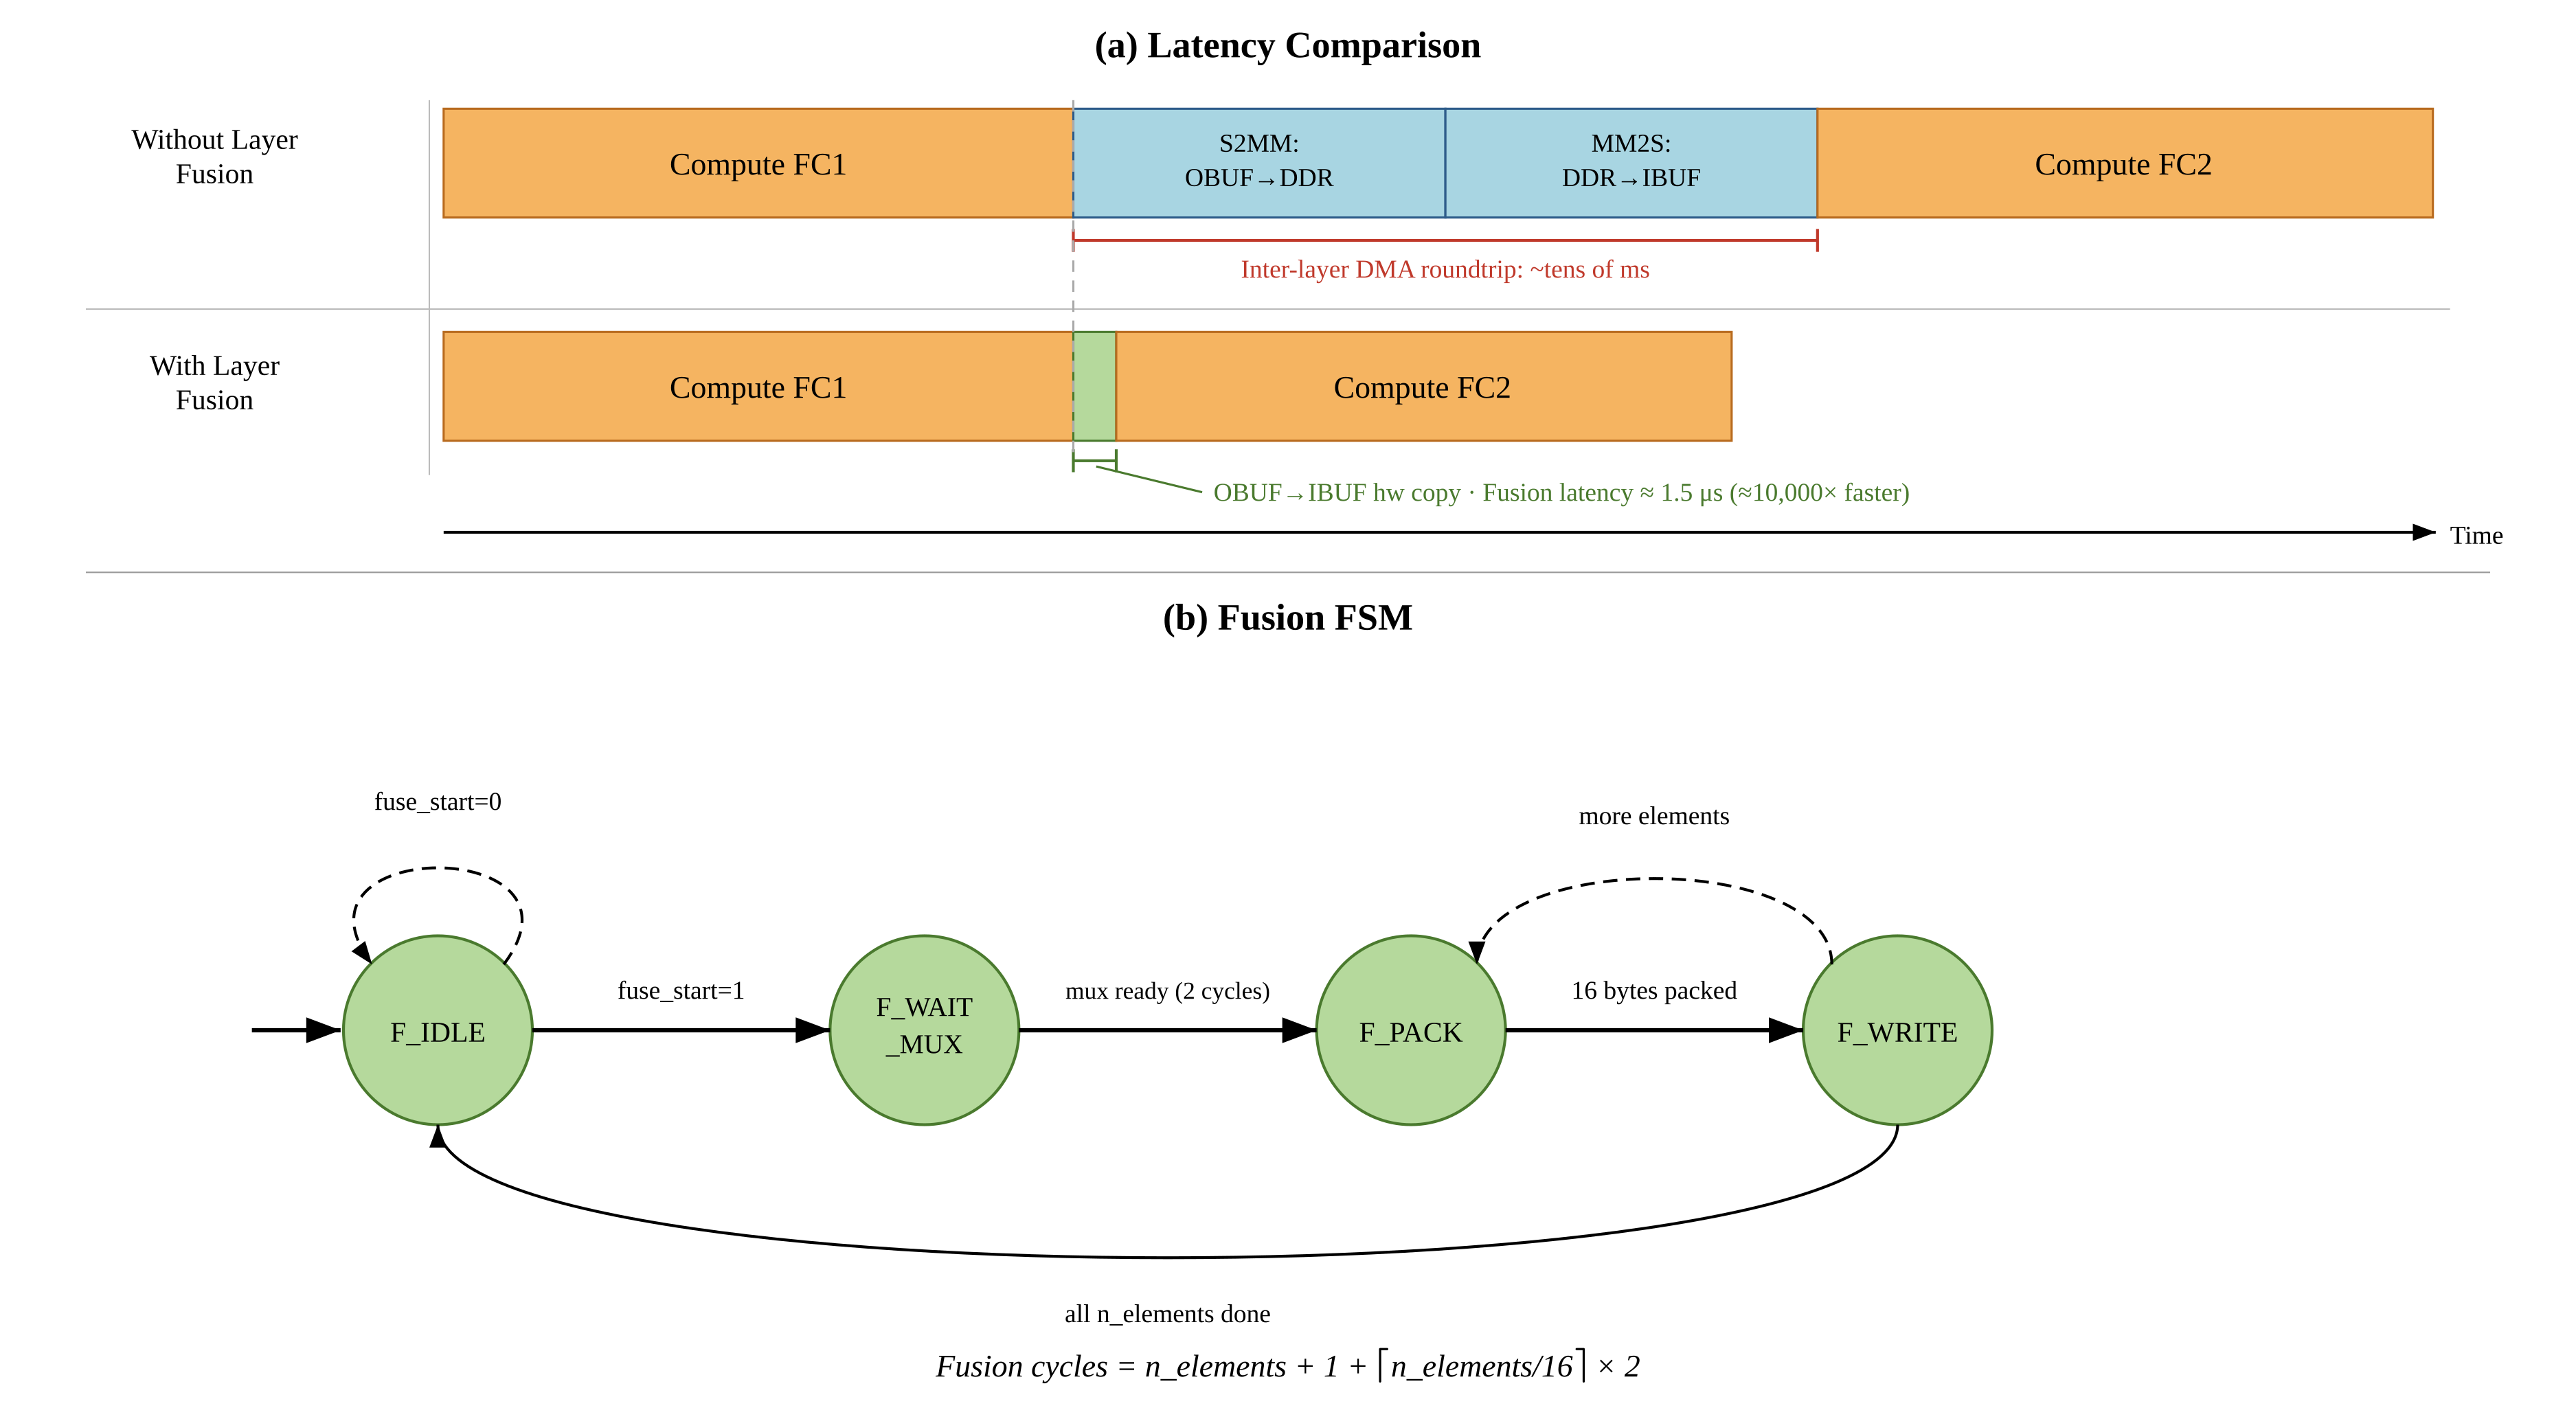
\includegraphics[width=\textwidth]{pics/2-8.png}
	\caption{层融合（Layer Fusion）机制。（a）时序对比：无融合时FC1$\to$FC2需经S2MM$\to$DDR$\to$MM2S往返（数十毫秒），融合时仅需OBUF$\to$IBUF硬件直拷（约1.5~$\mu$s）；（b）融合FSM状态转移（F\_IDLE$\to$F\_WAIT\_MUX$\to$F\_PACK$\to$F\_WRITE）。}
	\label{fig:layer_fusion}
\end{figure}

为支持多层权重共存，系统中增设了CSR\_WEIGHT\_BASE和CSR\_BIAS\_BASE偏移寄存器，使不同FC层的权重/偏置可在SRAM中存储于不同offset。FC1权重存于tile 0..N1-1，FC2权重存于tile N1..N1+N2-1，batch推理时仅需切换base寄存器即可在不同层之间切换。Python驱动侧的\texttt{setup\_fc\_fused\_pair()}预加载双layer权重，\texttt{infer\_fc\_fused\_batch()}实现批融合推理，无需每张图像重新加载FC2权重。

\subsection{流水线状态机与TILE\_SPLIT优化}

核心引擎的FSM包含多个状态，其中计算数据通路划分为以下流水线级：

\textbf{计算流水线}（每个input-block迭代）：
\begin{enumerate}
	\item \textbf{ST\_FETCH / ST\_WAIT\_SRAM}：发出BRAM读地址，等待权重SRAM输出（1 cycle latency）；
	\item \textbf{ST\_XEFF\_REG}：输入BRAM输出就绪 + 零点减法 → 锁存x\_eff\_reg；
	\item \textbf{ST\_MAC（或ST\_MAC\_Q0--Q3）}：cim\_tile计算 x\_eff\_reg $\times$ w\_tile\_reg → 锁存tile\_psum\_reg。当TILE\_SPLIT\_FACTOR=4时，该级拆分为4个子状态，每拍计算4列MAC；
	\item \textbf{ST\_COMPUTE}：psum\_accum += tile\_psum\_reg（寄存器加法）。
\end{enumerate}

\textbf{输出流水线}（每个output neuron，所有IB迭代完成后）：
\begin{enumerate}
	\setcounter{enumi}{4}
	\item \textbf{ST\_BIAS\_ADD → ST\_ACTIVATE}：加偏置 → ReLU激活；
	\item \textbf{ST\_STORE}：64位乘法（psum $\times$ requant\_mult）→ 锁存prod\_r；
	\item \textbf{ST\_SHIFT\_CLAMP → ST\_WRITE\_OBUF}：移位 + 舍入 + clamp → 写输出缓冲。
\end{enumerate}

上述计算流水线与输出流水线由核心引擎的FSM统一调度，其完整状态转移如图\ref{fig:core_fsm}所示，包含按input-block迭代的内层MAC循环与按output-block迭代的外层循环。

\begin{figure}[H]
	\centering
	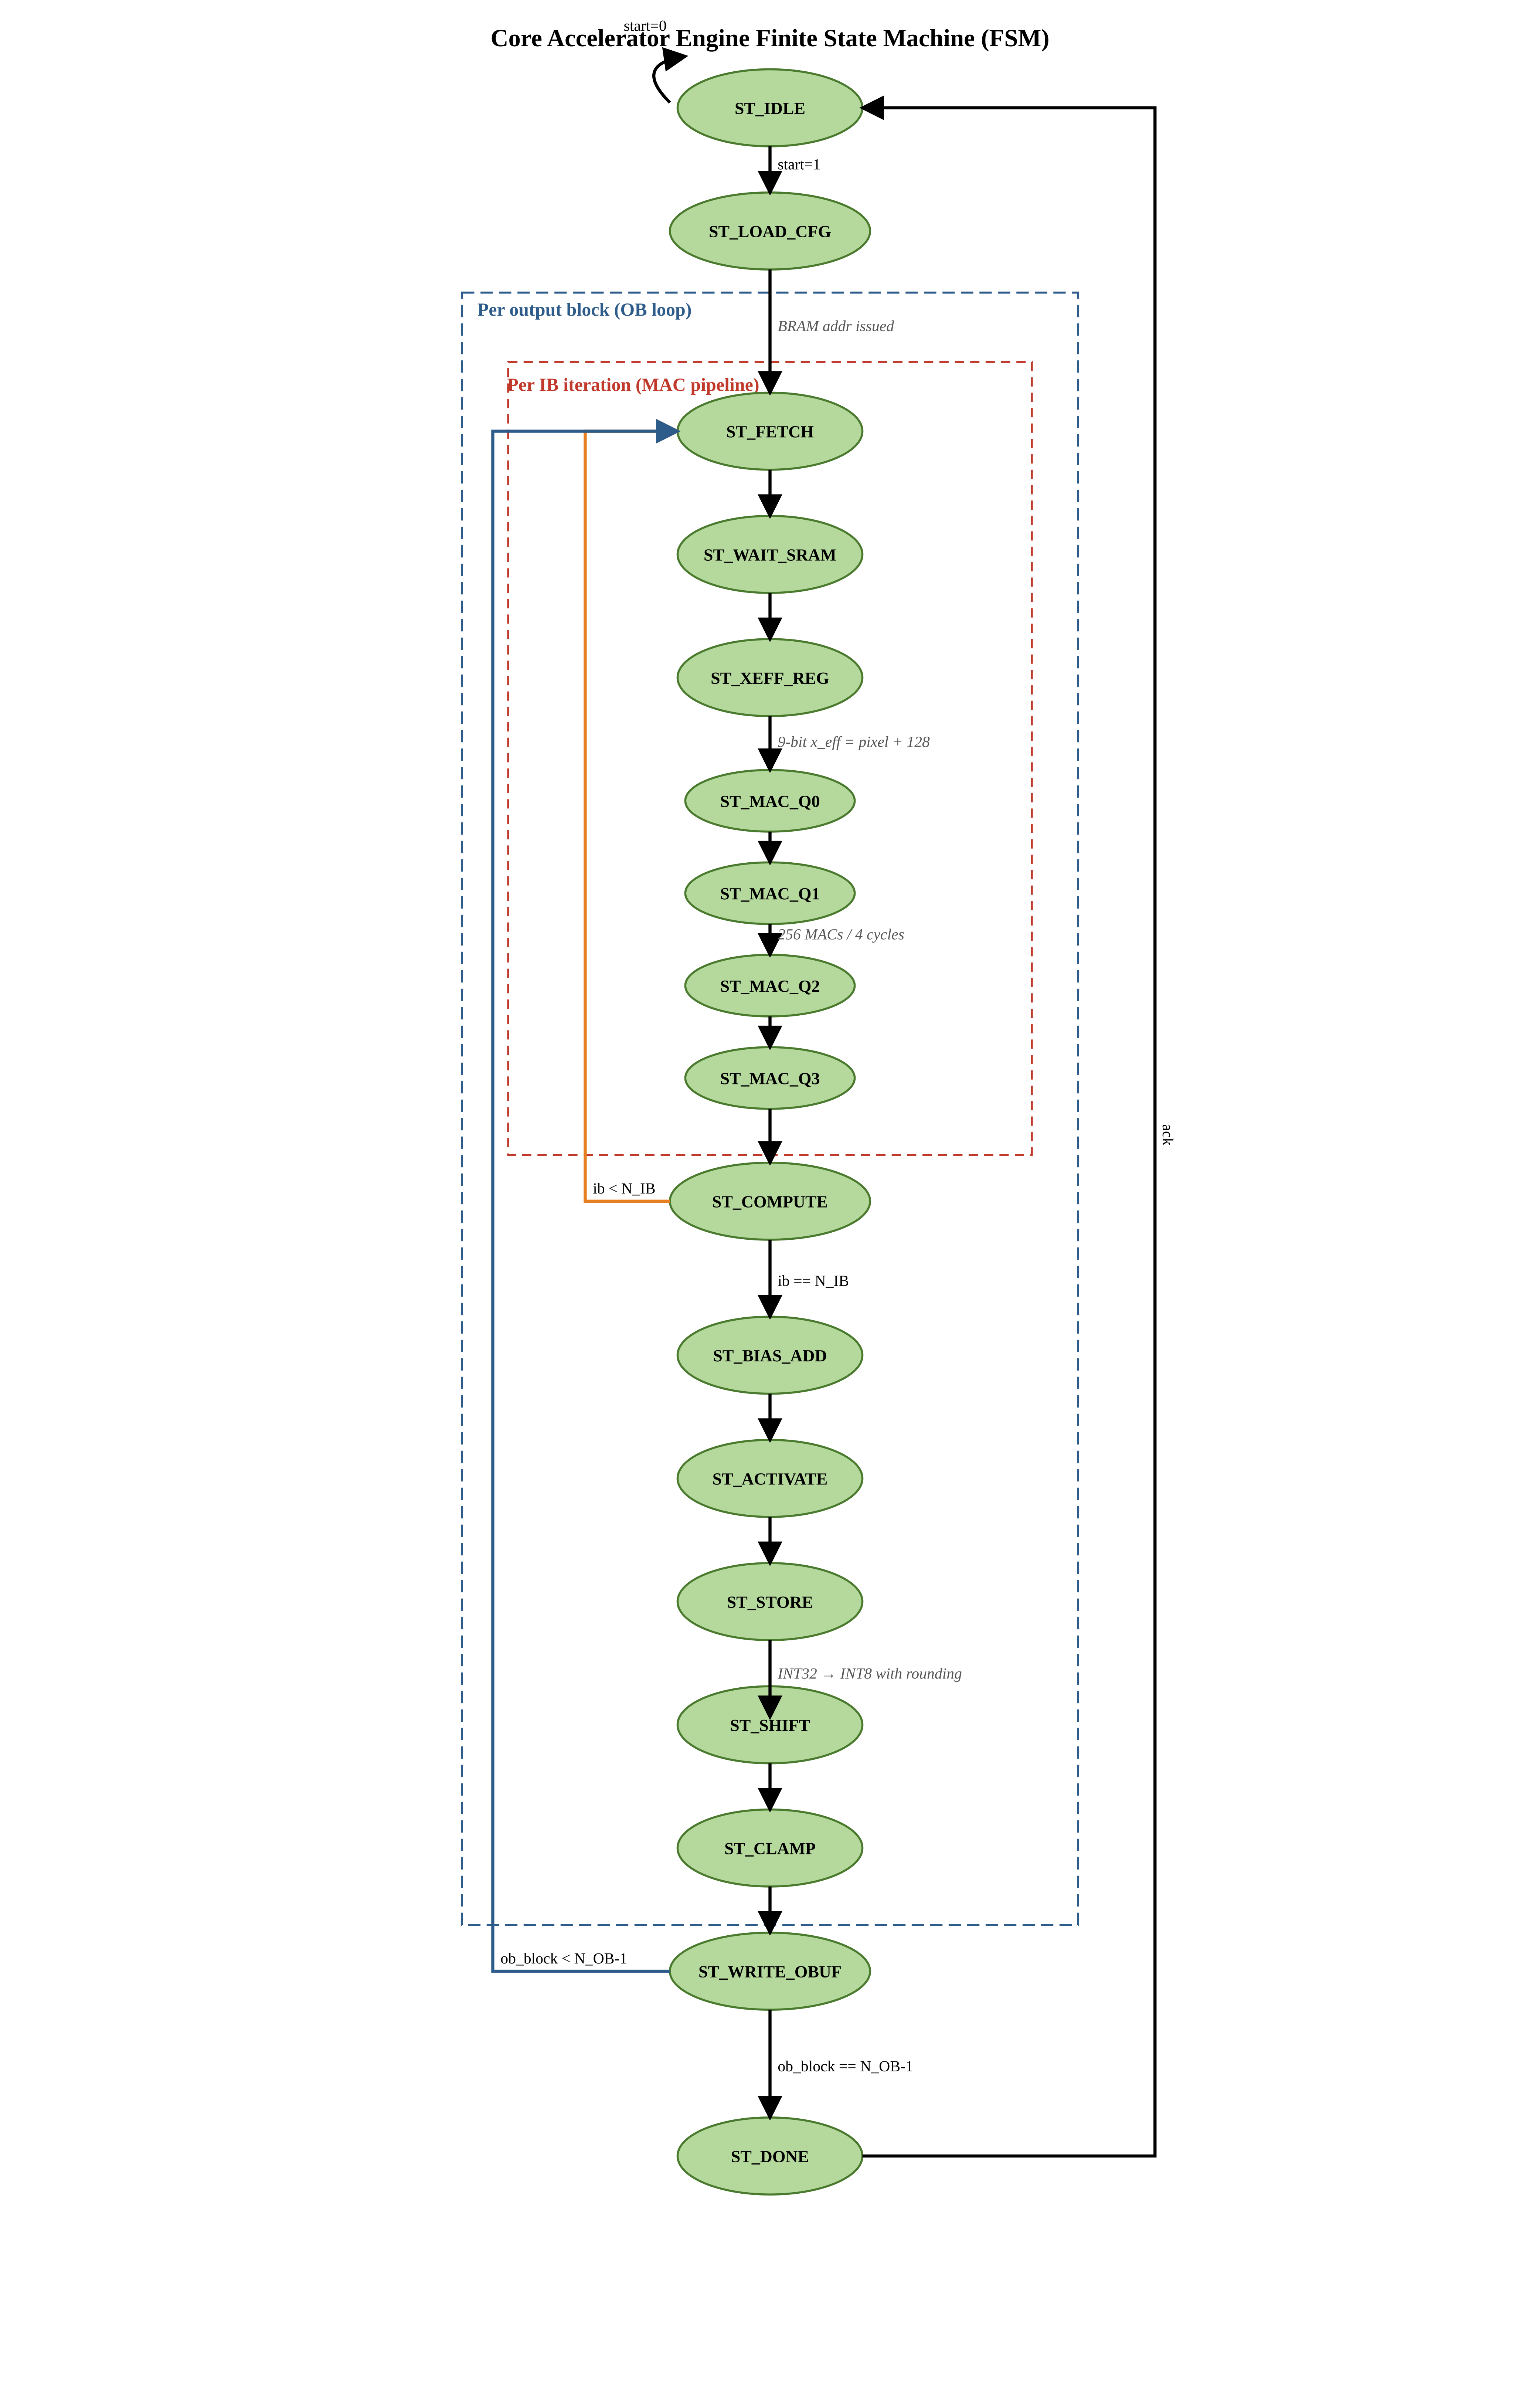
\includegraphics[width=0.95\textwidth]{pics/2-9.png}
	\caption{核心加速器引擎FSM状态转移图。内层循环（橙色，每IB迭代）完成取数、零点减法与MAC累加；外层循环（蓝色，每output block）完成偏置累加、激活、重量化与结果写回。单一FSM经CSR配置即可服务任意层维度。}
	\label{fig:core_fsm}
\end{figure}

为进一步提升时钟频率，后量化路径（原ST\_SHIFT\_CLAMP）被拆分为ST\_SHIFT（执行rounding加法并锁存pre\_shift\_r）和ST\_CLAMP（barrel shift + clamp至INT8范围）两级流水。该拆分将包含22个CARRY4进位链的组合路径分割为两段，每段关键路径控制在约10 ns以内，从而将时序收敛从60 MHz提升至80 MHz（WNS=+0.059 ns，时序完全收敛）。

\subsection{AXI4-Lite CSR接口}

系统通过AXI4-Lite slave接口与外部控制器（PS ARM或PicoRV32）交互，采用14位地址空间（16KB），CSR地址映射如表\ref{tab:csr_map}所示。

\begin{table}[H]
	\centering
	\caption{CSR地址映射}
	\label{tab:csr_map}
	\begin{tabular}{lcl}
		\toprule
		地址范围 & 偏移 & 功能 \\
		\midrule
		0x000--0x00C & & 控制/状态/IRQ寄存器 \\
		0x010--0x02C & & 层配置（IN\_DIM, OUT\_DIM, N\_IB, N\_OB, 量化参数） \\
		0x030--0x03C & & 性能计数器（cycle count, MAC count） \\
		0x040 & & argmax预测结果 \\
		0x050--0x058 & & Stream控制（DEST, LEN, STATUS） \\
		0x060--0x06C & & Result/S2MM控制 + Ping-Pong CTRL \\
		0x070--0x080 & & Layer Fusion控制 + Weight/Bias Base偏移 \\
		0x100--0x2FF & & Logits回读窗口 \\
		\bottomrule
	\end{tabular}
\end{table}

为更直观地展示CSR地址空间的布局，图\ref{fig:csr_map}以地址条形图的形式给出了各功能区段的分布。

\begin{figure}[H]
	\centering
	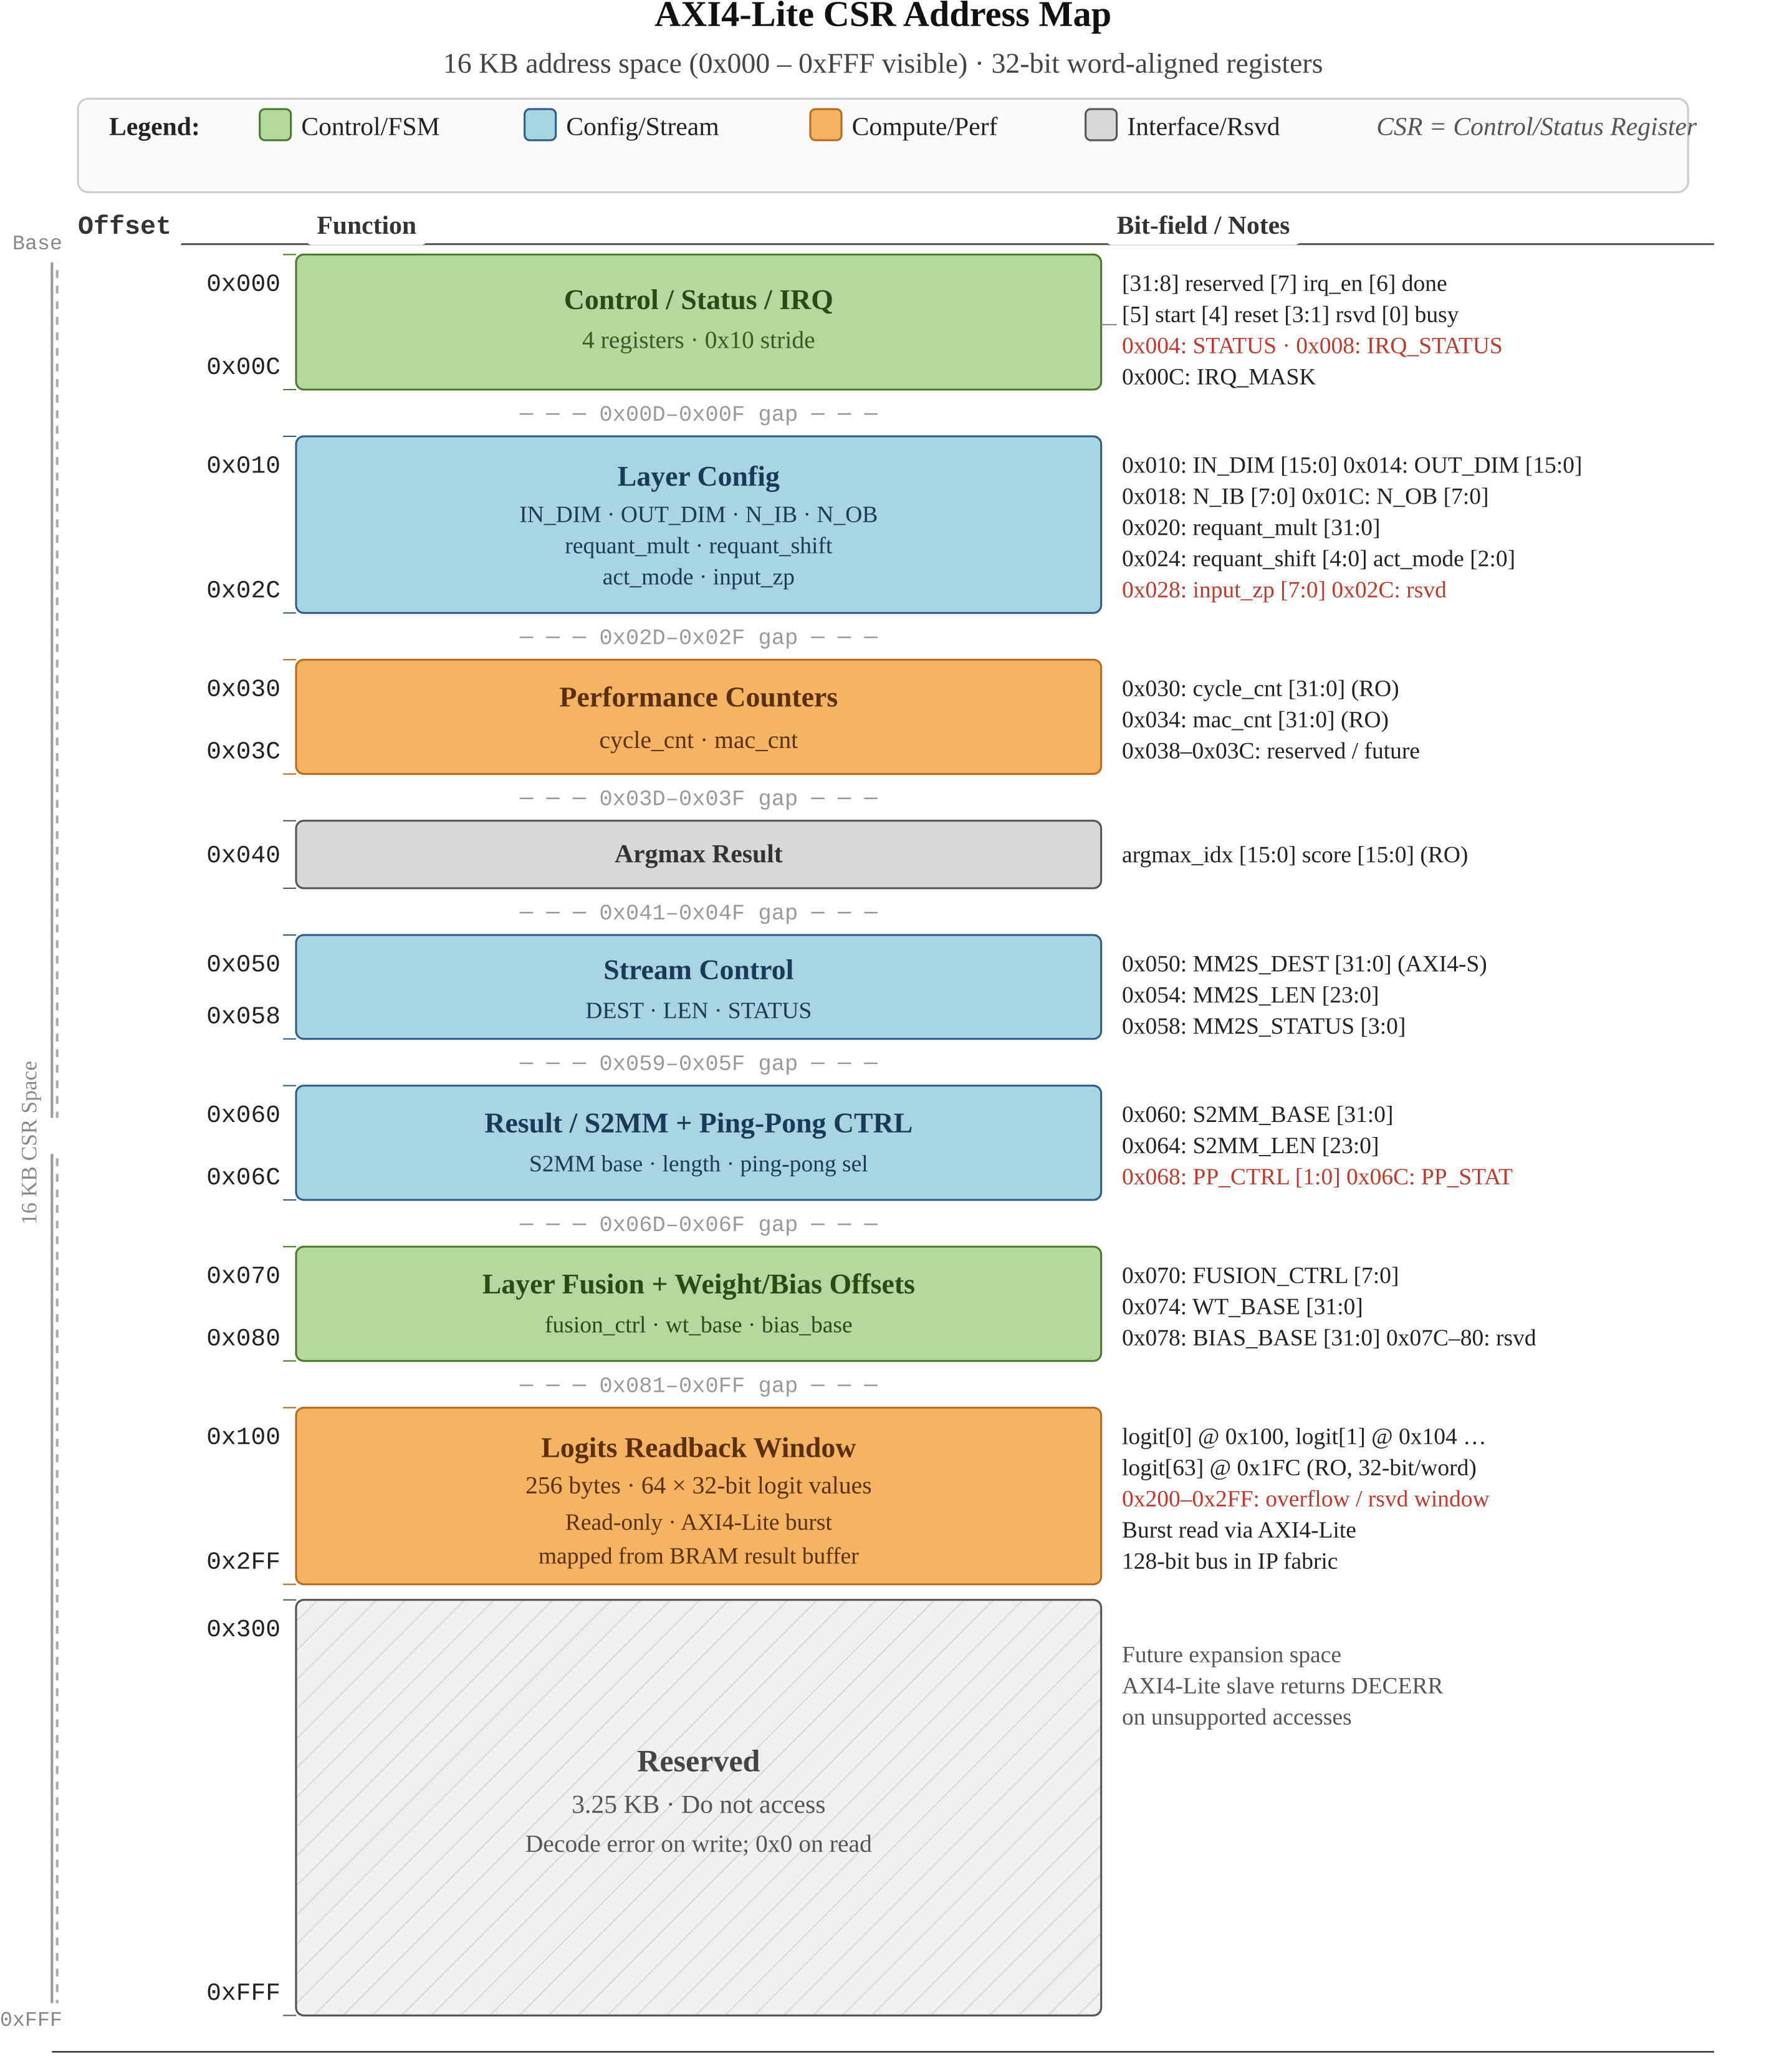
\includegraphics[width=0.7\textwidth]{pics/2-10.png}
	\caption{AXI4-Lite CSR地址空间映射条形图。低地址端为控制/状态、层配置与性能计数器，中段为stream/ping-pong/layer-fusion控制与权重/偏置基址偏移，高地址端为logits回读窗口与保留区。}
	\label{fig:csr_map}
\end{figure}

% ====================================================================
\section{PicoRV32 RISC-V软核集成}
% ====================================================================

\subsection{设计动机}

前述ARM PS控制模式下，CIM加速器依赖ARM Cortex-A9进行推理调度与数据搬运。为实现纯PL侧自主推理能力，本设计集成PicoRV32开源RISC-V软核（YosysHQ，MIT License）替代ARM PS。其优势包括：

\begin{itemize}
	\item 单文件实现（\texttt{picorv32.v}），RV32IM指令集；
	\item 资源开销低且反直觉地轻量：PicoRV32核心约1,500个LUT，完整子系统（含bridge、UART TX、FW/Result BRAM接口）因去除了axi\_dma及关联AXI互连，总LUT反而比ARM模式净减少351个，以更少的逻辑资源实现更自主的控制；
	\item 成熟的native memory interface，适合直接桥接到CIM CSR。
\end{itemize}

最终目标是让CIM加速器在纯PL中自主运行推理，不依赖PS控制。

PicoRV32系统与ARM版本共享相同的CIM IP RTL（含TILE\_SPLIT\_FACTOR=4、双缓冲、Layer Fusion、WEIGHT\_BASE/BIAS\_BASE等全部优化），因此同样工作于100 MHz。以下各节给出的都是100 MHz实测数据。

\subsection{系统架构}

PicoRV32集成后的系统顶层架构如图\ref{fig:rv32_soc}所示：PS仅承担固件加载与结果回读，PicoRV32子系统（核心 + bridge + 双端口FW/Result BRAM + AXI GPIO复位控制）在纯PL侧自主驱动推理，右侧CIM IP保持零RTL改动。系统设计要点包括：

（1）\textbf{CIM IP不做修改}：PicoRV32通过mini AXI master发送与ARM完全相同的AXI事务，CIM IP的AXI slave接口无需任何改动，确保了与ARM控制路径的完全兼容。

（2）\textbf{双端口FW BRAM}：固件通过PS侧AXI写入FW BRAM port B，而不是烧写到bitstream中。这使得每次更换测试图片无需重新生成bitstream，只需重新加载firmware.hex。FW BRAM容量32KB，足以容纳784→16→10小型MLP模型的权重数据与C固件代码（共约18.5KB）。

（3）\textbf{Result BRAM}：PicoRV32将推理结果（预测类别、logits、magic标记）写入Result BRAM，PS通过AXI读取结果。这避免了PL侧UART与PS侧USB的连接性问题。

（4）\textbf{CPU复位控制}：PS通过AXI GPIO控制cpu\_rst\_n信号，实现hold → write firmware → release的操作流程。

\begin{figure}[H]
	\centering
	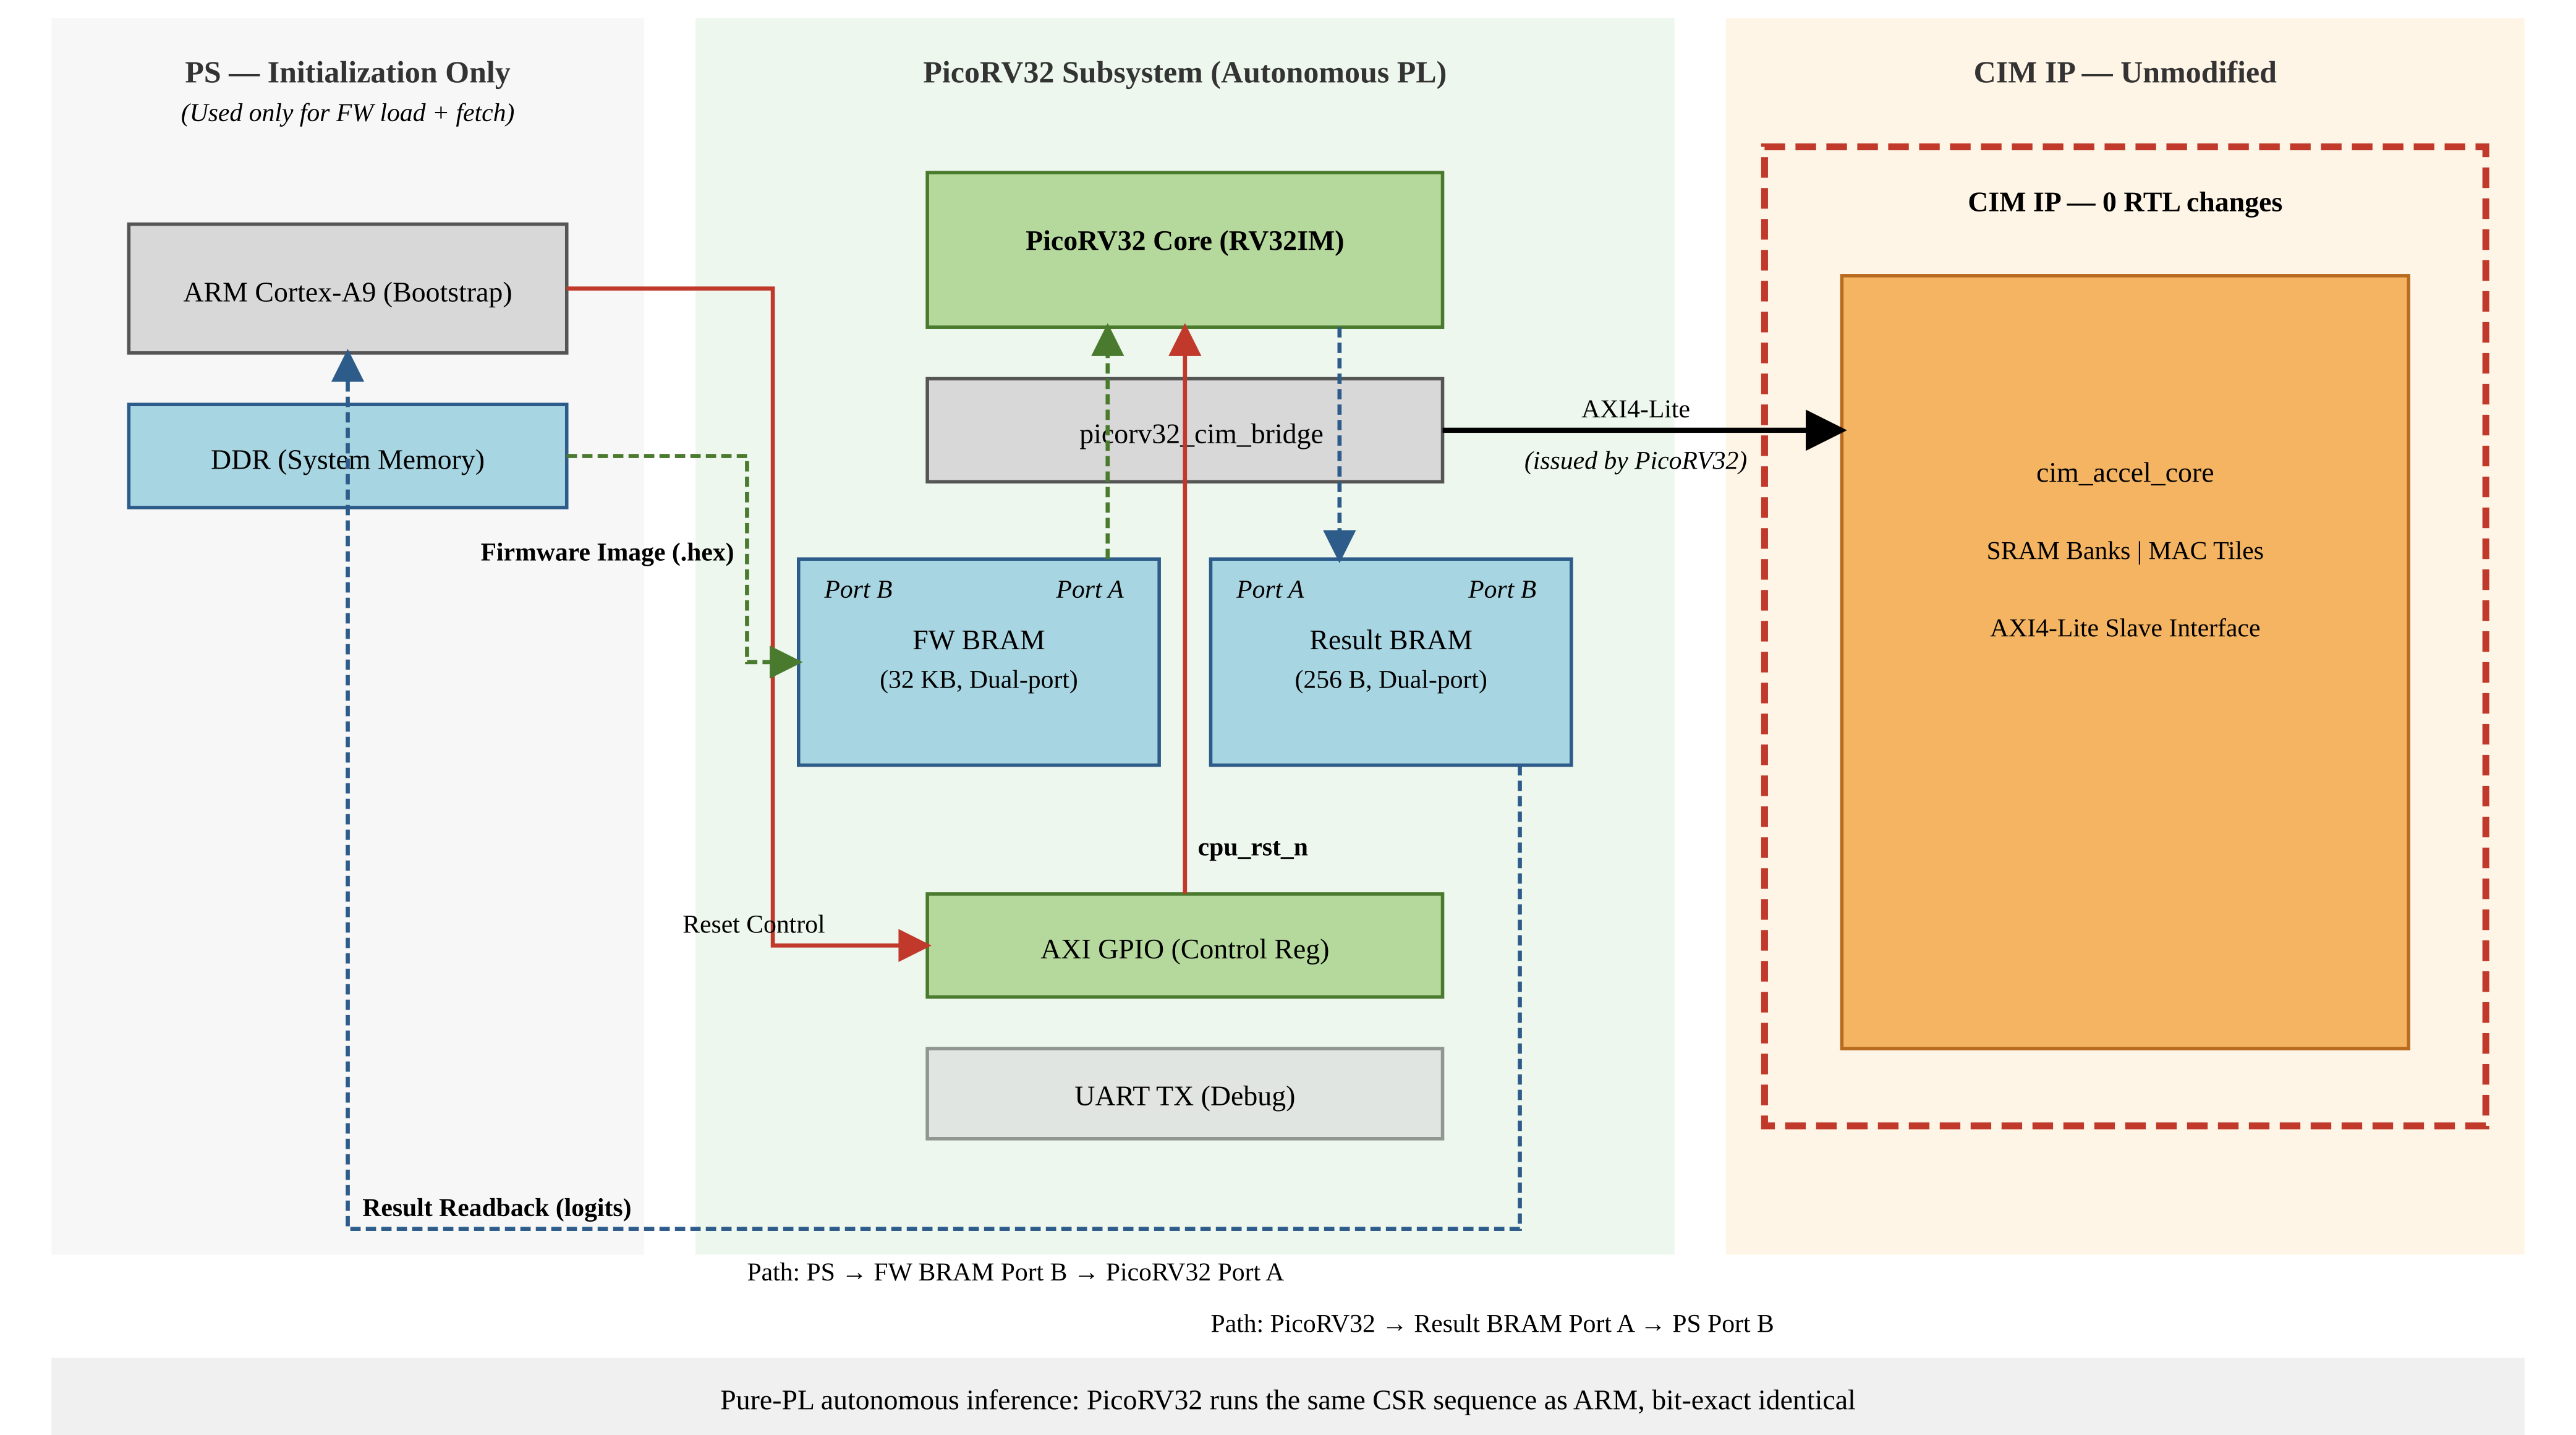
\includegraphics[width=\textwidth]{pics/3-1.png}
	\caption{PicoRV32 + CIM SoC系统框图。左侧PS仅用于固件加载与结果回读；中央PicoRV32子系统经bridge与双端口FW/Result BRAM实现纯PL侧自主推理；右侧CIM IP零RTL改动，PicoRV32发出与ARM完全相同的AXI4-Lite事务。}
	\label{fig:rv32_soc}
\end{figure}

\subsection{Bus Bridge与地址映射}

\texttt{picorv32\_cim\_bridge}模块将PicoRV32的native memory interface桥接到各外设，地址映射如下表所示：

\begin{table}[H]
	\centering
	\caption{PicoRV32地址映射}
	\begin{tabular}{lcl}
		\toprule
		地址范围 & 大小 & 设备 \\
		\midrule
		0x0000\_0000 -- 0x0000\_7FFF & 32KB & FW BRAM (port A) \\
		0x4000\_0000 -- 0x4000\_3FFF & 16KB & CIM CSR / 存储窗口 \\
		0x8000\_0000 & 4B & UART TX数据寄存器 \\
		0x8000\_0004 & 4B & UART TX状态寄存器 \\
		0xC000\_0000 -- 0xC000\_00FF & 256B & Result BRAM (port A) \\
		\bottomrule
	\end{tabular}
\end{table}

Bridge根据地址高位进行译码，对CIM CSR区域的访问转换为AXI读写事务。PicoRV32访问CIM的流程与ARM通过MMIO访问完全等价，固件中的CSR读写函数直接对应AXI事务。该32位地址空间的整体布局如图\ref{fig:rv32_addrmap}所示。

\begin{figure}[H]
	\centering
	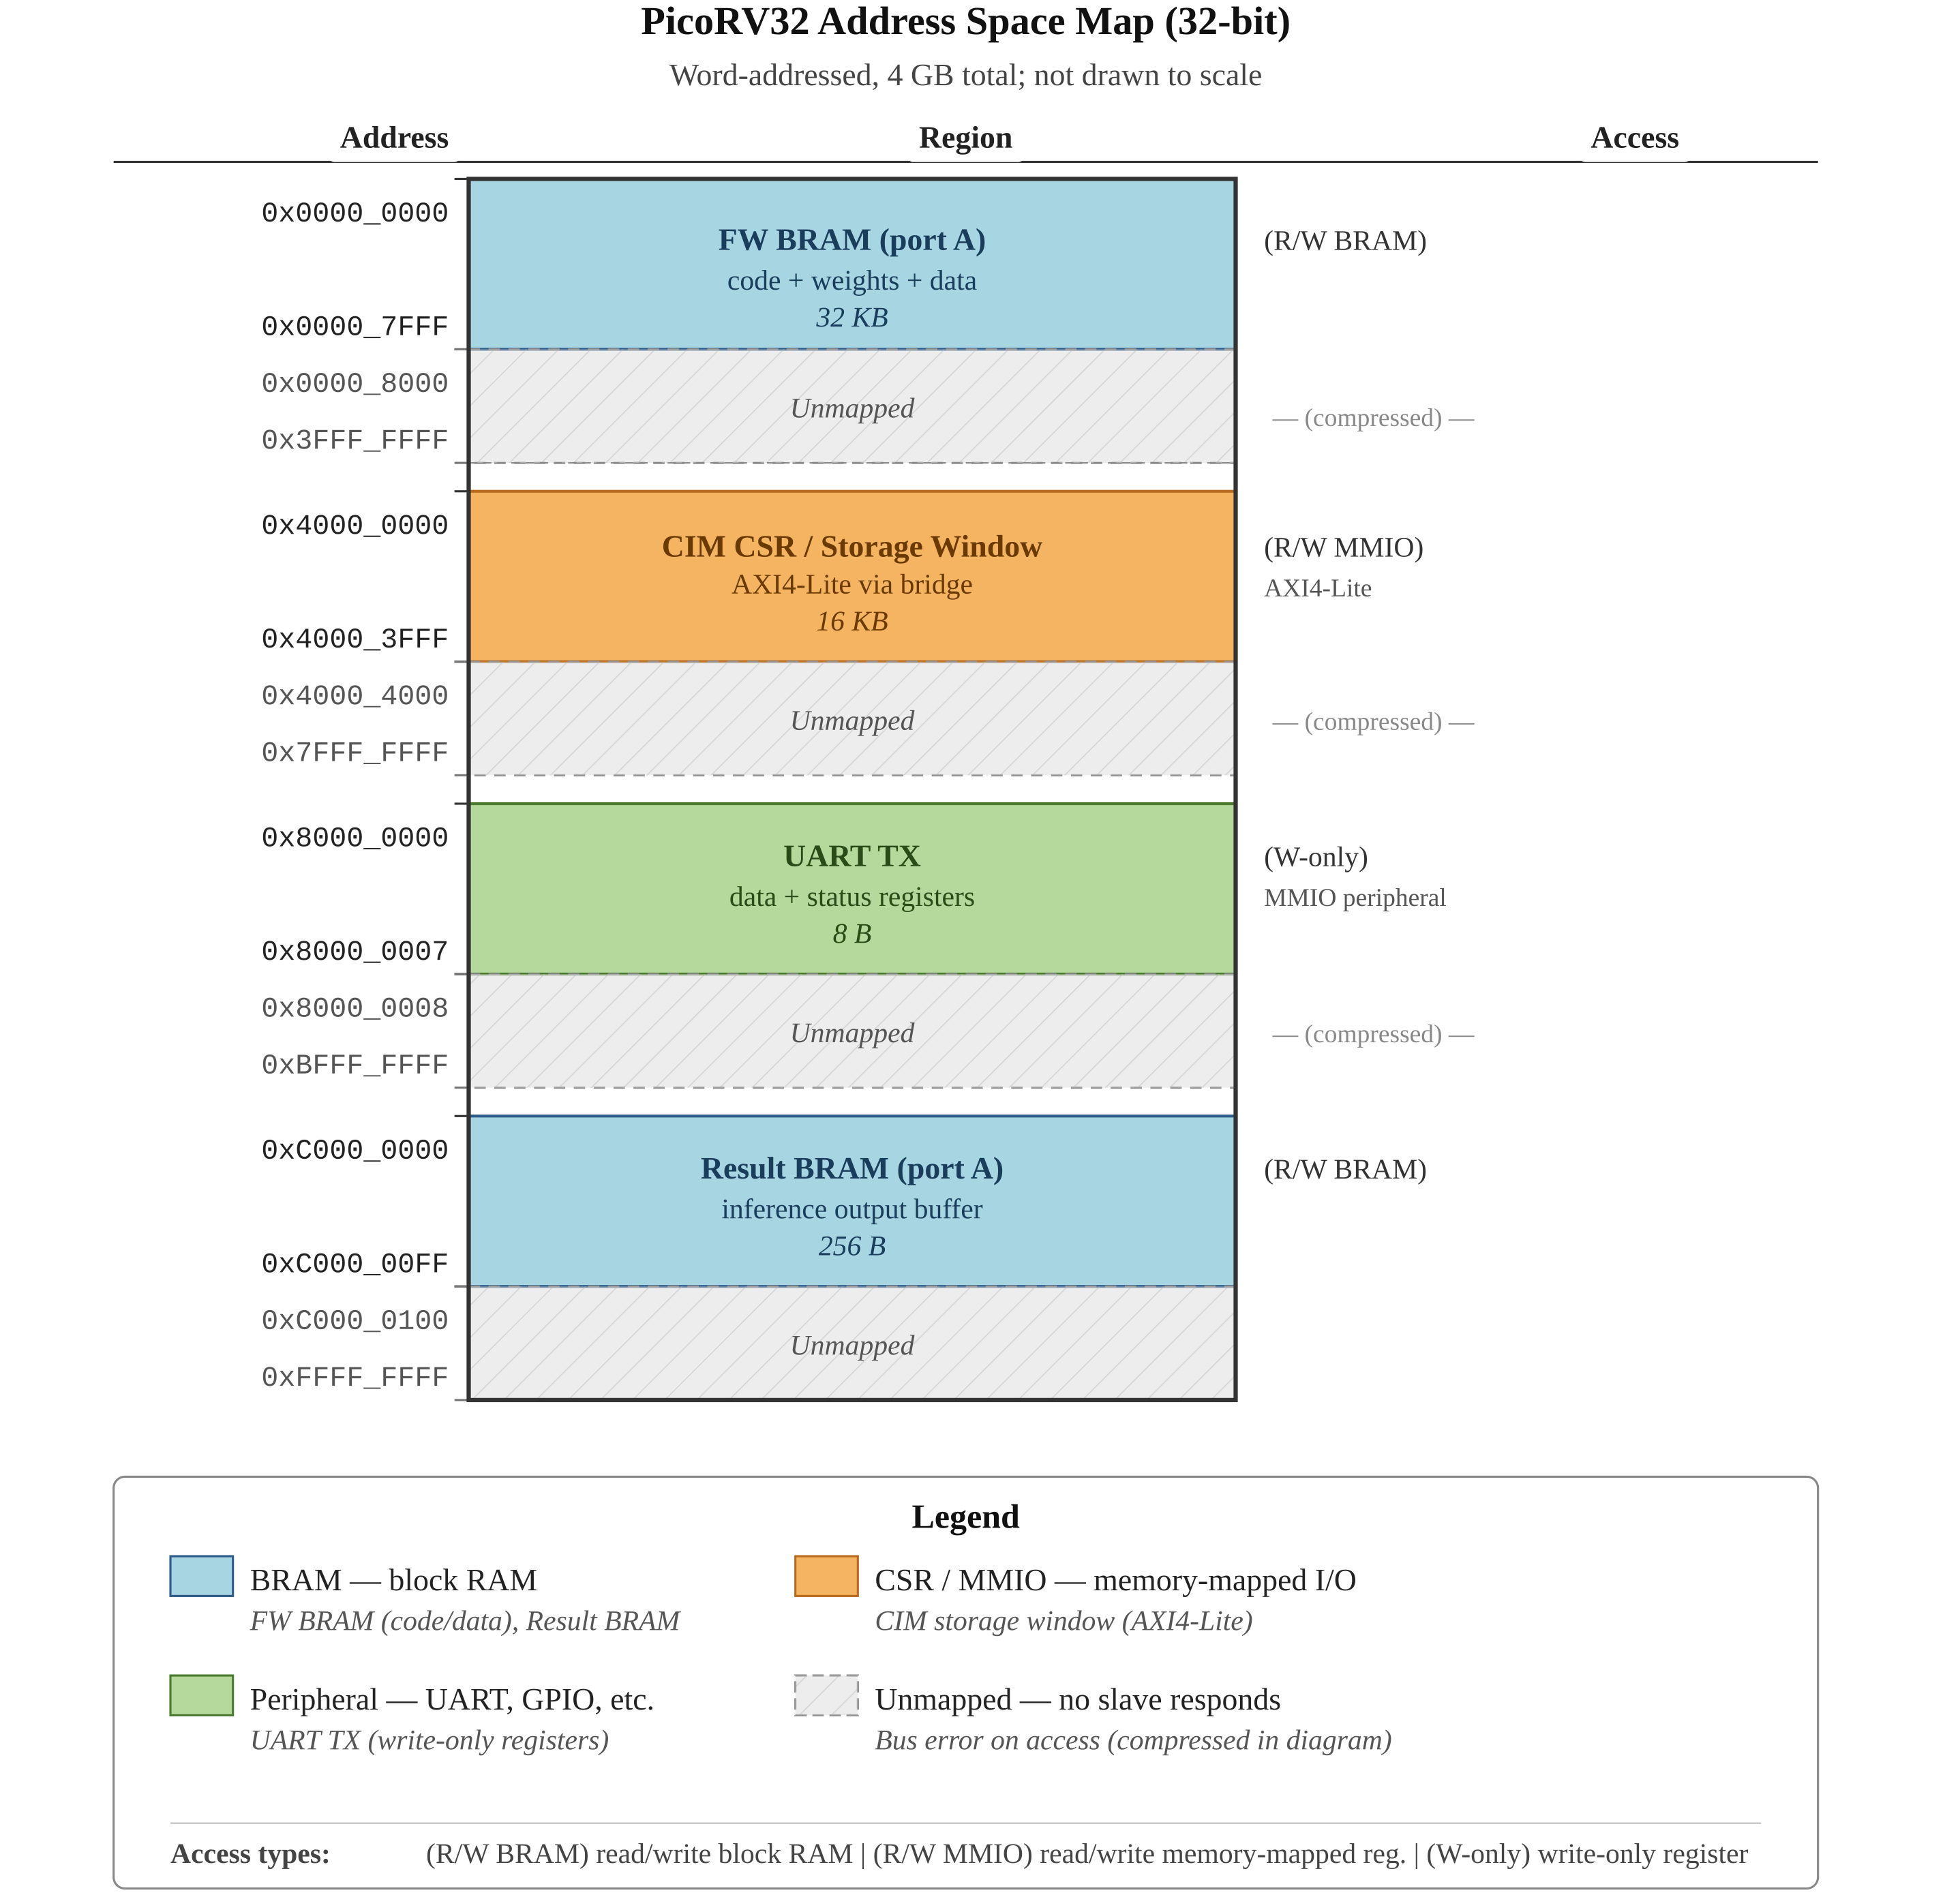
\includegraphics[width=0.62\textwidth]{pics/3-2.png}
	\caption{PicoRV32地址空间布局。低地址段为FW BRAM（代码+权重+数据），0x4000\_0000段映射至CIM CSR/存储窗口（经bridge转为AXI4-Lite），0x8000\_0000段为UART TX，0xC000\_0000段为Result BRAM，其余为未映射区。}
	\label{fig:rv32_addrmap}
\end{figure}


\subsection{模型规模约束}

虽然PicoRV32反而节省了LUT资源，但是固件中需要放入32KB FW BRAM，模型规模受到限制(将MLP模型缩小为784→16→10)。FW BRAM中需要存储：C固件代码、权重数据（INT8打包）、偏置数据（INT32）与输入数据。对于784→16→10的小型MLP模型，数据量约为：

\begin{equation}
	784 \times 16 \times 1 + 16 \times 10 \times 1 + (16 + 10) \times 4 + 784 \times 1 \approx 14.5\text{KB}
\end{equation}

加上C固件代码约4KB，总计约18.5KB，可以放入32KB BRAM中。该模型在MNIST测试集上INT8量化推理准确率超过95\%。

% ====================================================================
\section{FPGA验证与性能评估}
% ====================================================================

\subsection{验证方法学}

本项目建立了"Python golden model → VCS仿真 → PYNQ上板"三层一致的验证方法学：

\textbf{第一层：Python bit-accurate参考模型}。\texttt{golden\_model.py}以纯整数算术实现与硬件完全相同的计算流程（零点减法、MVM、偏置累加、ReLU、重量化），输出hex格式测试向量供RTL仿真和板级验证使用。

\textbf{第二层：VCS RTL仿真}。采用"单元级→阵列级→系统级"分层验证策略：
\begin{itemize}
	\item \textbf{tb\_cim\_tile}：CIM Tile单元测试，103个测试向量（含3个定向测试与100个随机向量），验证MAC运算正确性；
	\item \textbf{tb\_cim\_accel\_core}：系统级MVM测试，覆盖随机向量与边界用例（全零、全$-128$、最大维度等）；
	\item \textbf{tb\_mnist\_e2e}：MNIST端到端测试，784→128→10两层MLP，与golden model逐元素对比。
\end{itemize}

通过\texttt{run\_regression.sh}脚本一键运行全部测试并汇总PASS/FAIL结果。

\textbf{第三层：PYNQ-Z2上板验证}。将bitstream与hwh文件部署到PYNQ板，通过Python驱动程序（\texttt{cim\_driver.py}的\texttt{CIMModel}类），加载真实MNIST手写数字图片，逐层执行推理并与golden model对比。

上述三层验证的整体流程与层间bit-exact对比关系如图\ref{fig:verify_flow}所示。

\begin{figure}[H]
	\centering
	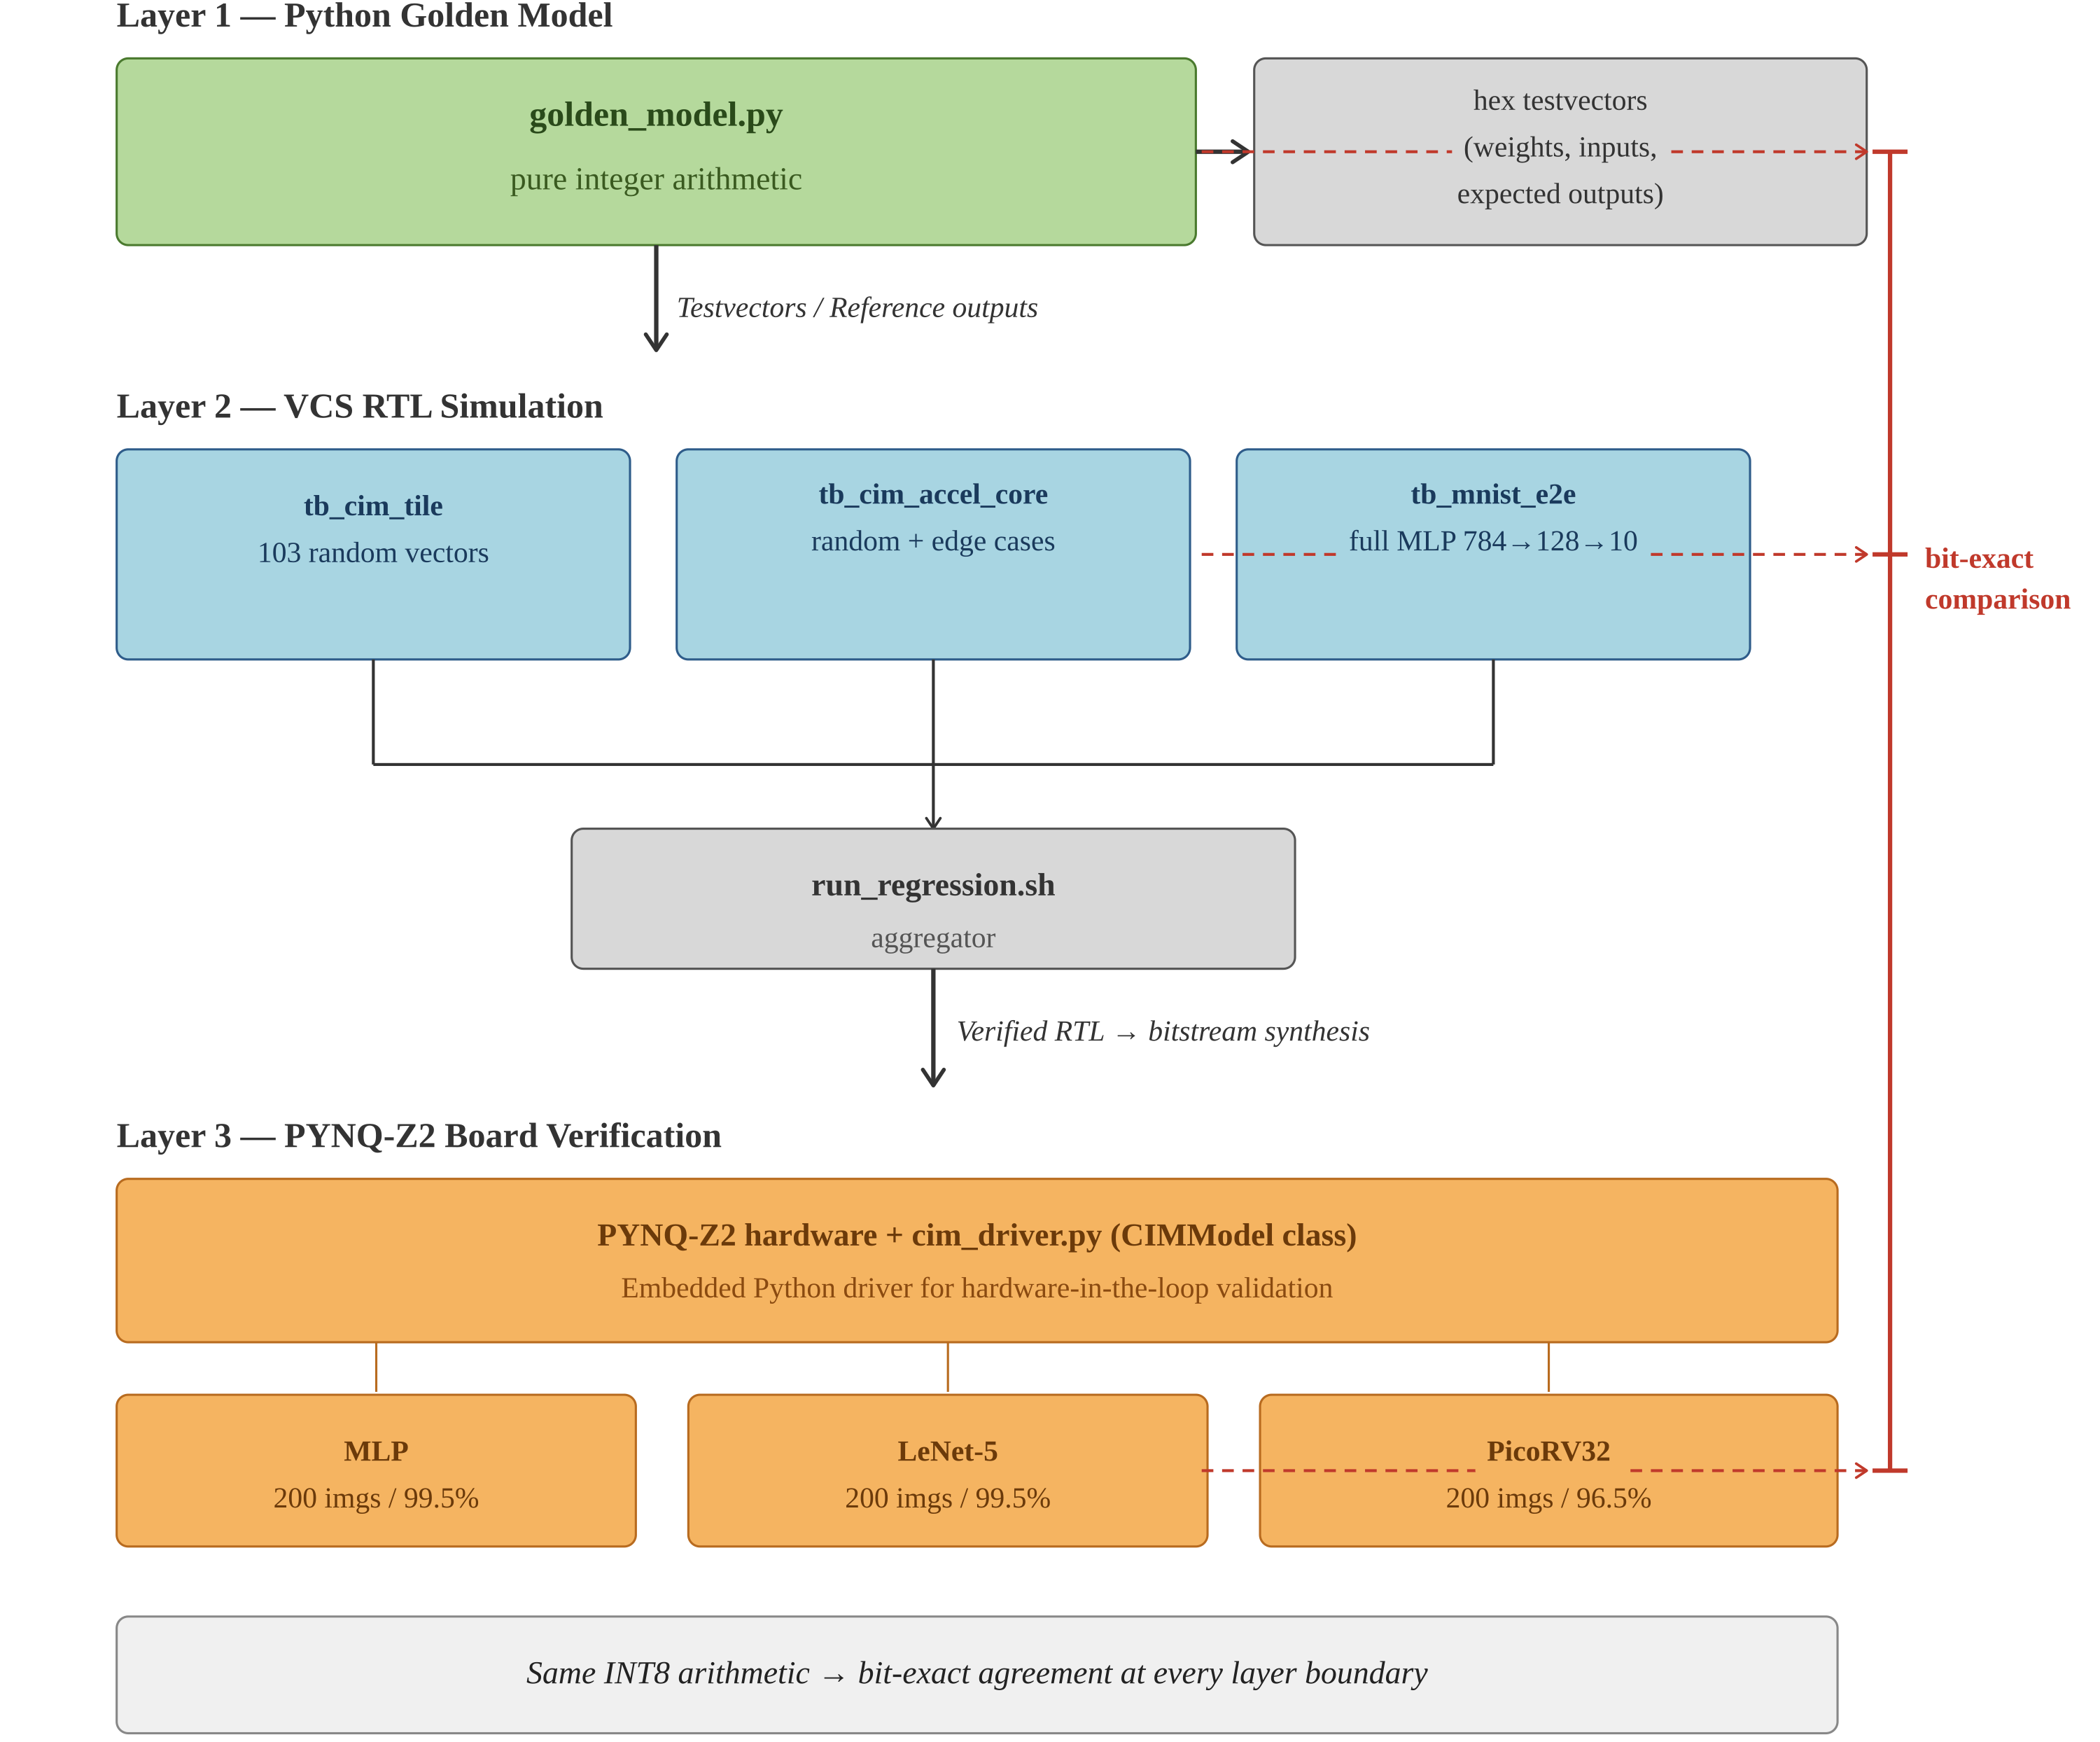
\includegraphics[width=0.9\textwidth]{pics/4-1.png}
	\caption{三层一致的验证方法学。Python golden model生成hex测试向量，经VCS RTL仿真（tile/core/端到端三级testbench）验证后综合为bitstream并在PYNQ-Z2上板验证；三层之间在每个边界均做bit-exact对比。}
	\label{fig:verify_flow}
\end{figure}

\subsection{PYNQ-Z2综合结果}

设计在Vivado 2024.2中针对Zynq-7020（xc7z020clg400-1）进行综合与实现。表\ref{tab:util_final}列出了最终配置（Phase B双缓冲 + Layer Fusion + TILE\_SPLIT\_FACTOR=4，100 MHz）下的资源使用量。

\begin{table}[H]
	\centering
	\caption{CIM SoC资源占用（最终配置，100 MHz，PYNQ-Z2）}
	\begin{tabular}{lcccc}
		\toprule
		资源类型 & 使用量 & 可用量 & 占用率 \\
		\midrule
		Slice LUT & 17,374 & 53,200 & 32.66\% \\
		Slice Register (FF) & 10,911 & 106,400 & 10.25\% \\
		Block RAM (36Kb) & 123.5 & 140 & 88.21\% \\
		DSP48E1 & 220 & 220 & 100.00\% \\
		\bottomrule
	\end{tabular}
	\label{tab:util_final}
\end{table}

时序方面，100 MHz（10 ns周期）构建的WNS为$-0.911$ ns，存在一定时序违例，但是室温下功能正常，可以正常运行；80 MHz（12.5 ns周期）构建实现完全时序收敛（WNS=+0.059 ns）。关键路径位于x\_eff\_reg→DSP48E1→LUT/CARRY4→tile\_psum\_q0\_reg，主要受限于16路MAC拆分后仍存在的DSP级联与布线延迟。

Vivado功耗分析表明，系统总片上功耗为2.283 W（动态2.114 W，静态0.169 W）。其中CIM IP动态功耗为0.559 W，仅占总动态功耗的26.4\%，其内部主要贡献来自DSP48（0.188 W）、互连信号（0.153 W）与Block RAM（0.113 W）；PS7（ARM Cortex-A9双核 + DDR控制器）消耗1.538 W，占总动态功耗的72.8\%，是系统功耗的主导因素。PicoRV32模式下总功耗为2.240 W，CIM子系统动态功耗为0.537 W，相比ARM模式略有下降，主要归因于PL侧LUT与FF逻辑资源的减少。图\ref{fig:util_bar}以条形图形式直观对比了两种控制模式下的资源占用。其中DSP48在两种模式下均达到100\%，是限制并行度（PAR\_OB）进一步提升的瓶颈（详见§\ref{sec:future_work}）。

\begin{figure}[H]
	\centering
	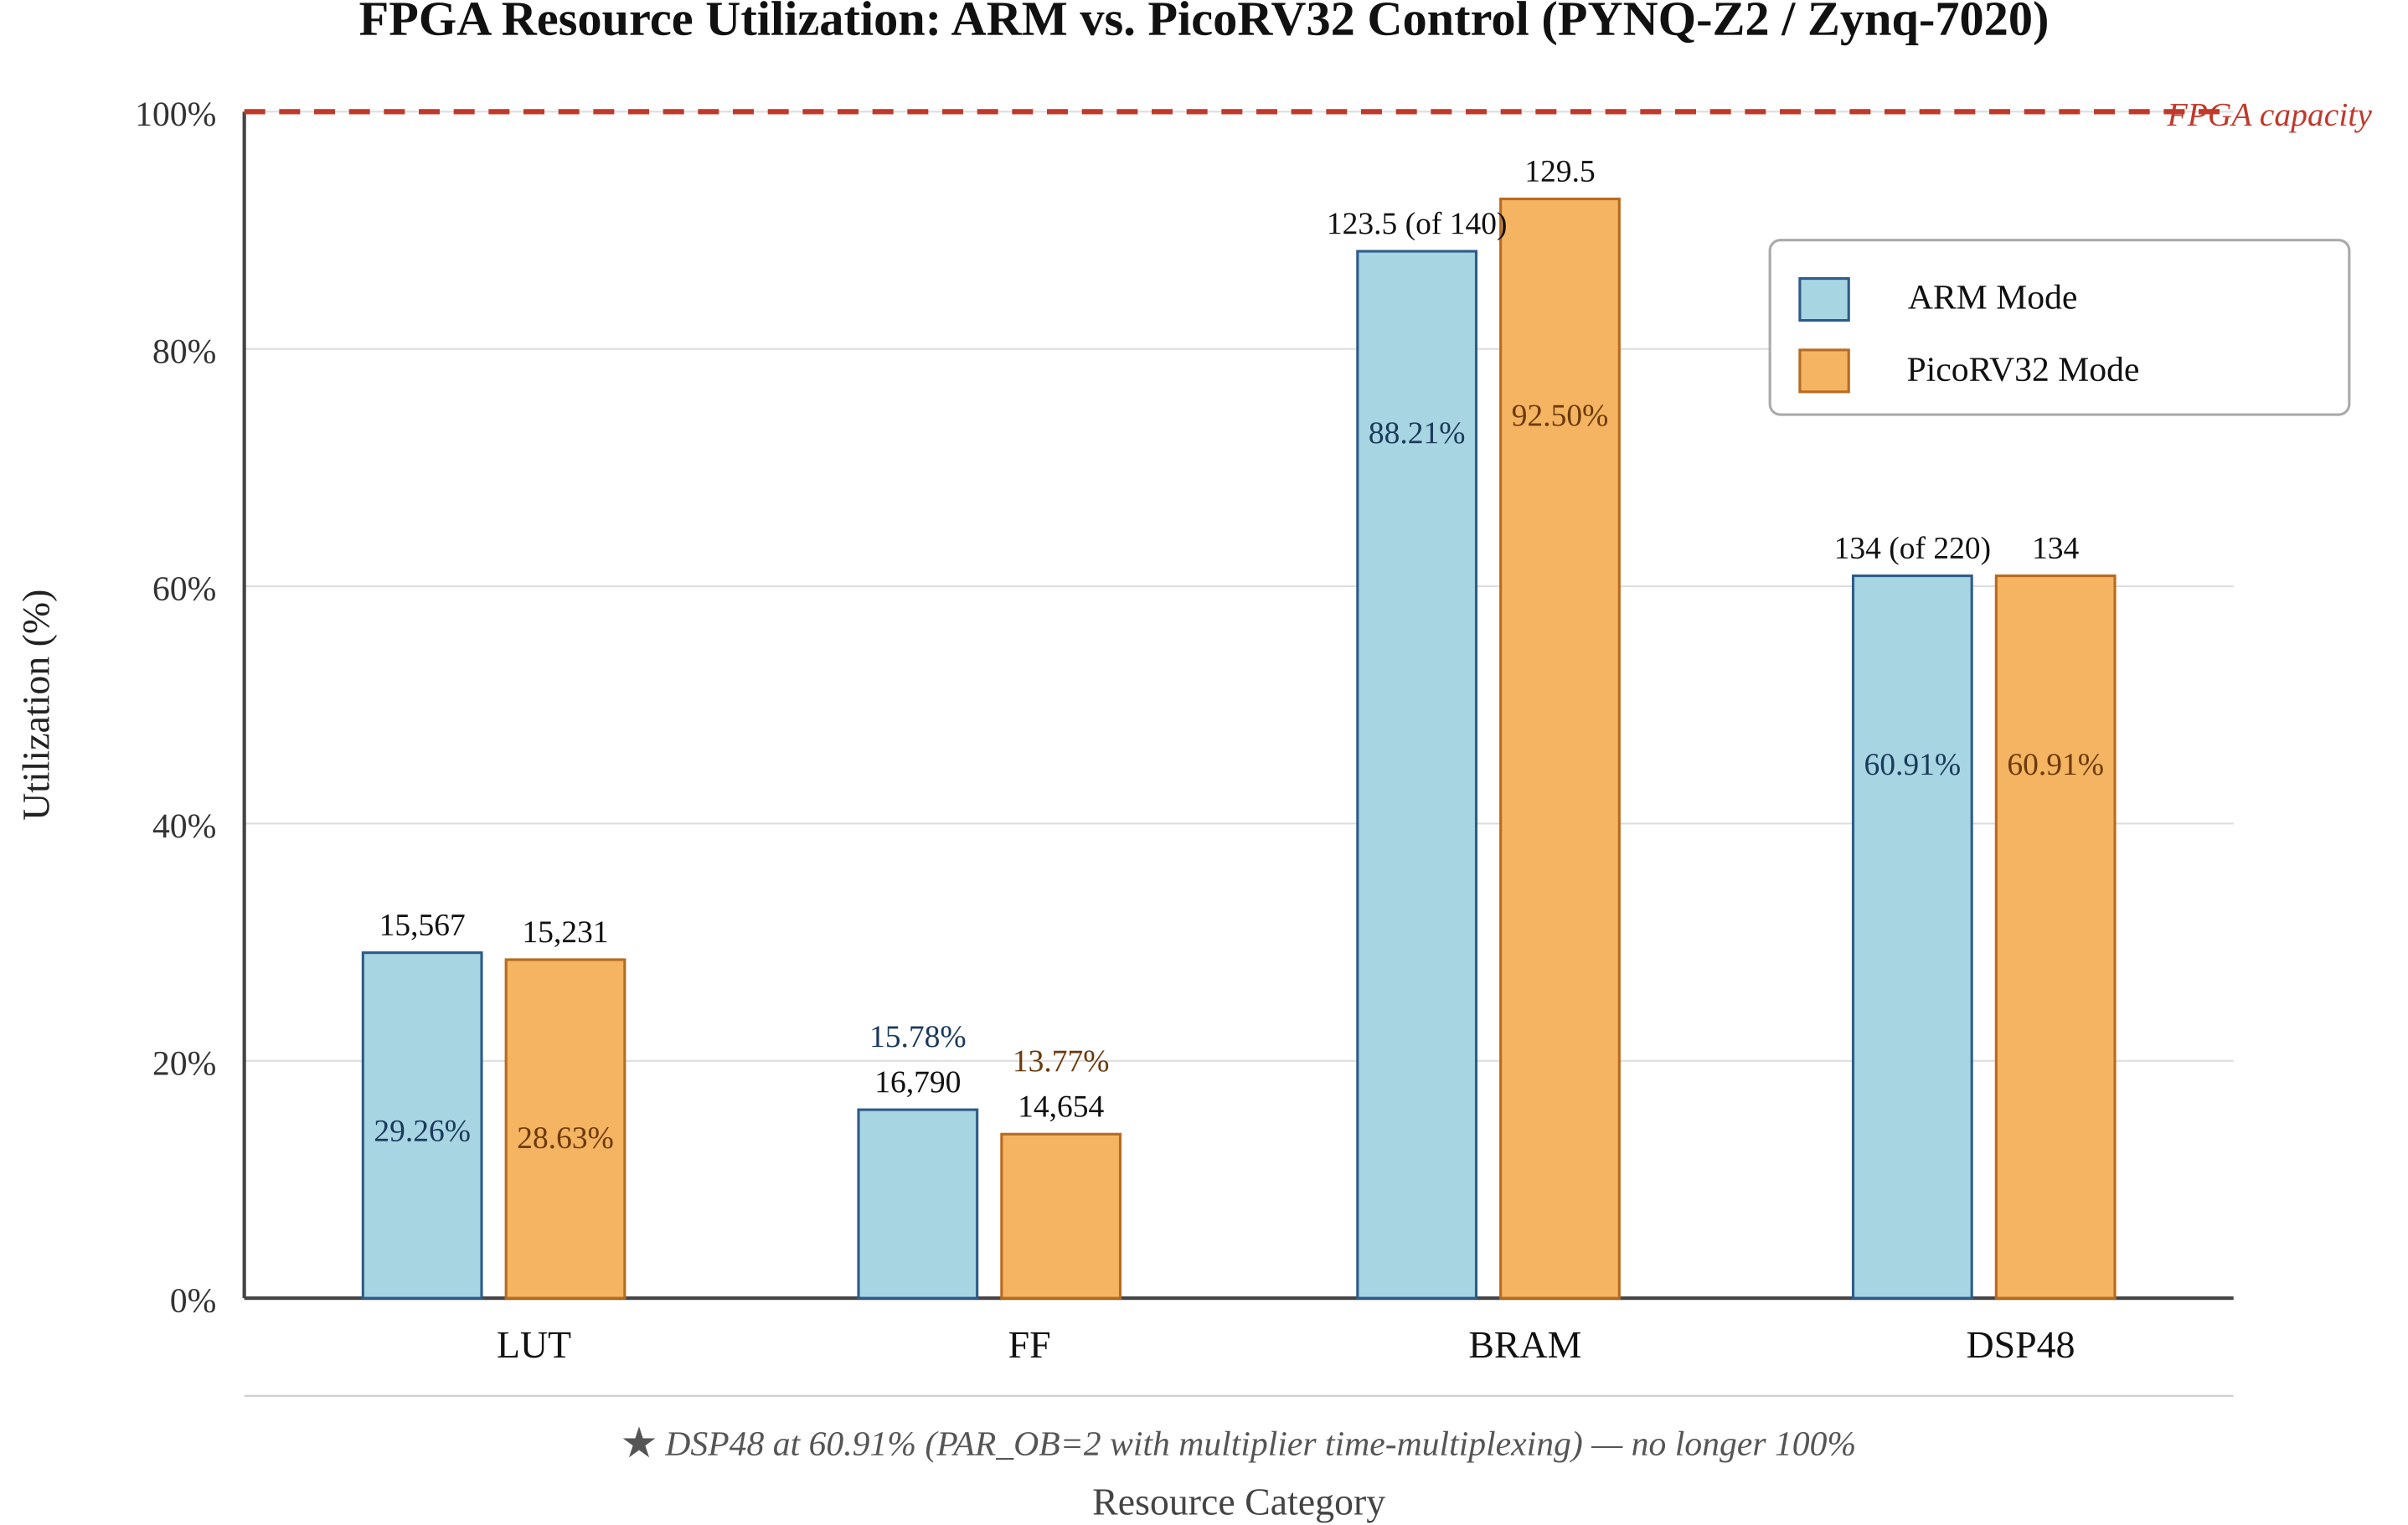
\includegraphics[width=0.85\textwidth]{pics/4-3.png}
	\caption{两种控制模式下的FPGA资源占用对比（PYNQ-Z2/Zynq-7020）。ARM模式与PicoRV32模式均为100 MHz实测数据，具体数值分别见表\ref{tab:util_final}与表\ref{tab:util_rv32}。DSP48在两种模式下均为100\%。}
	\label{fig:util_bar}
\end{figure}


\subsection{MLP网络推理验证}

在ARM控制模式下，使用784→128→10两层MLP网络（INT8量化，200张MNIST测试图片板级分类准确率99.0\%）进行上板验证。表\ref{tab:mlp_perf}给出了各层的推理周期数与MAC操作数。

\begin{table}[H]
	\centering
	\caption{MLP推理性能（最终配置，100 MHz）}
	\begin{tabular}{lccc}
		\toprule
		层 & 维度 & 周期数 & MAC操作数 \\
		\midrule
		FC1 & 784→128 & 3,136 & 100,352 \\
		FC2 & 128→10 & 146 & 2,048 \\
		\midrule
		总计 & & 3,282 & 102,400 \\
		\bottomrule
	\end{tabular}
	\label{tab:mlp_perf}
\end{table}

单幅推理的硬件计算延迟为：
\begin{equation}
	T_{\text{MLP, compute}} = \frac{3282}{100 \times 10^6} = 32.8\,\mu\mathrm{s}
\end{equation}

端到端延迟则包含Python驱动开销与DMA传输。表\ref{tab:mlp_arm_configs}给出了ARM控制模式下MLP网络在三种数据通路配置下的200张实测端到端性能。

\begin{table}[H]
	\centering
	\caption{ARM模式下MLP（784→128→10）200张端到端性能对比}
	\label{tab:mlp_arm_configs}
	\begin{tabular}{lcccc}
		\toprule
		配置 & 总时间（s） & ms/img & fps & 准确率 \\
		\midrule
		MMIO-only & 99.68 & 498.41 & 2.01 & 99.00\% \\
		DMA & 5.59 & 27.93 & 35.80 & 99.00\% \\
		DMA + batch & \textbf{0.40} & \textbf{2.00} & \textbf{499.6} & 99.00\% \\
		\bottomrule
	\end{tabular}
\end{table}

从MMIO-only到DMA+batch，端到端加速约249倍。在200张真实MNIST手写数字测试中，硬件输出与Python golden model逐元素完全一致（100\% bit-exact），分类准确率99.0\%（198/200）；2张错分均与golden model预测一致，源于INT8量化精度损失。Layer Fusion启用后，FC1→FC2的层间延迟从DMA S2MM+MM2S往返的数十毫秒降至约1.5 $\mu$s。

\subsection{LeNet-5 CNN推理验证}

LeNet-5是一个包含2个卷积层、2个最大池化层和3个全连接层的经典CNN。由于CIM硬件本身只支持MVM运算，卷积层通过软件侧im2col变换转化为矩阵乘法后喂给硬件引擎。im2col将卷积的滑窗操作展开为一个大矩阵，使得$\text{col\_len} = C_{in} \times K \times K$作为MVM的输入维度。MaxPool层在Python侧以向量化方式实现。LeNet-5的网络结构及各层在CIM上的软硬件执行映射如图\ref{fig:lenet5}所示。表\ref{tab:lenet5_perf}列出了各层的推理周期数。

\begin{figure}[H]
	\centering
	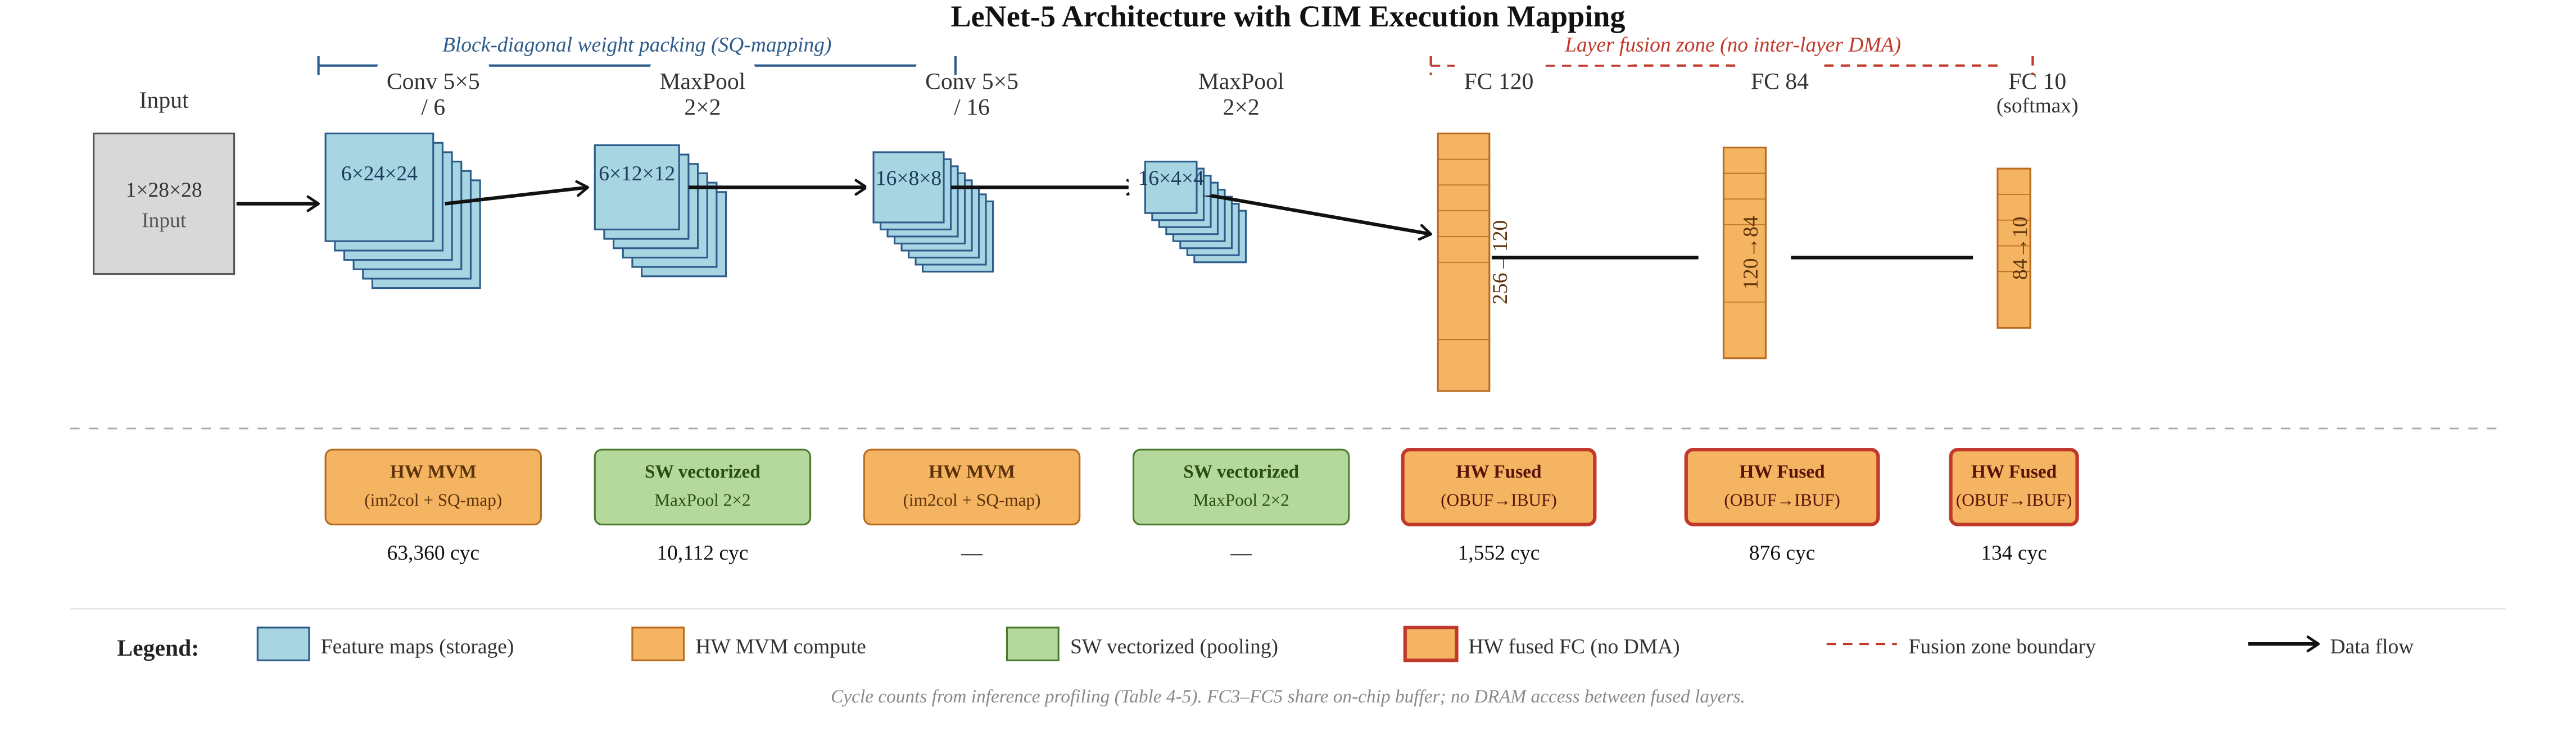
\includegraphics[width=\textwidth]{pics/4-4.png}
	\caption{LeNet-5网络结构与CIM执行映射。上方为各层维度，下方标注执行方式：卷积层经im2col+SQ-mapping在硬件MVM上执行，池化层在Python侧向量化执行，连续FC层通过OBUF$\to$IBUF层融合在硬件上执行。}
	\label{fig:lenet5}
\end{figure}

\begin{table}[H]
	\centering
	\caption{LeNet-5各层推理周期数（最终配置，100 MHz）}
	\begin{tabular}{lcccc}
		\toprule
		层 & 类型 & 维度 & 平均周期数 \\
		\midrule
		conv1 & Conv 5×5 & 1×28×28→6×24×24 & 63,360 \\
		conv2 & Conv 5×5 & 6×12×12→16×8×8 & 10,112 \\
		fc3 & FC & 256→120 & 1,552 \\
		fc4 & FC & 120→84 & 876 \\
		fc5 & FC & 84→10 & 134 \\
		\midrule
		总计 & & & 76,034 \\
		\bottomrule
	\end{tabular}
	\label{tab:lenet5_perf}
\end{table}

在200张真实MNIST手写数字测试中：
\begin{itemize}
	\item 硬件分类准确率（vs 标签）：99.5\%（199/200）
	\item 与Python golden model的bit-exact一致率：100.0\%（200/200）
	\item 计算错误数：0
\end{itemize}

200张图片中唯一的"错误"分类（img\_0018，标签3预测为8）与Python golden model的预测完全一致，说明这是INT8量化精度损失导致的，而非硬件计算错误。全部200张图片的全部层输出均与Python参考模型bit-exact一致，验证了硬件实现的正确性。


\subsection{SQ-mapping：块对角权重打包的卷积映射优化}
\label{sec:sqmapping}

在LeNet-5这类小卷积核网络中，直接把im2col得到的每个输出像素逐一送入MVM引擎会严重浪费CIM阵列的利用率。以Conv1层（$1\times5\times5\to6$）为例，单次MVM的有效输入维度仅为$\text{col\_len} = C_{in}\times K_h\times K_w = 25$，而硬件支持的最大输入维度为1536，利用率不足$25/1536\approx 1.6\%$；同时单次MVM产生$C_{out}=6$个输出神经元，输出侧利用率同样极低。这种"瘦长矩阵挤在大阵列里"的映射方式使得每次硬件调用的建立与DMA开销被完全暴露，无法被有效均摊。

针对这一问题，本文引入并应用了\textbf{块对角权重打包}（SQ-mapping）这一已有的软件映射优化方法：当$\text{col\_len}\times C_{out}$远小于硬件容量时，把$k_{\text{pack}}$个输出像素的im2col列与权重一起打包到同一次MVM调用中。SQ-mapping的基本思想并非本文首创，本文的贡献在于将其与本设计的硬件维度上限（MAX\_IN\_DIM/MAX\_OUT\_DIM）、双缓冲乒乓批处理流程及Python驱动侧的权重预打包相结合，给出在本平台上的具体参数化实现与bit-exact验证。原始权重矩阵$W\in\mathbb{Z}^{C_{out}\times \text{col\_len}}$沿对角线复制$k_{\text{pack}}$份构造块对角矩阵：

\begin{equation}
	W_{\text{packed}} = \begin{bmatrix}
		W & & & \\
		& W & & \\
		& & \ddots & \\
		& & & W
	\end{bmatrix} \in \mathbb{Z}^{(k_{\text{pack}}\cdot C_{out})\times (k_{\text{pack}}\cdot \text{col\_len})}
\end{equation}

输入侧同时将$k_{\text{pack}}$个输出像素对应的im2col列串联成长向量。一次硬件调用即可同时得到$k_{\text{pack}}\cdot C_{out}$个输出神经元，再按$C_{out}$拆回$k_{\text{pack}}$组像素结果。打包因子由硬件维度上限决定：

\begin{equation}
	k_{\text{pack}} = \min\!\left(\left\lfloor\frac{\text{MAX\_IN\_DIM}}{\text{col\_len}}\right\rfloor,\ \left\lfloor\frac{\text{MAX\_OUT\_DIM}}{C_{out}}\right\rfloor\right)
\end{equation}

SQ-mapping的块对角打包思想如图\ref{fig:sqmapping}所示：左侧逐像素映射时瘦长权重矩阵仅占据阵列极小一角，利用率不足5\%；右侧将$k_{\text{pack}}$份权重沿对角线复制构成块对角矩阵，一次MVM调用即可并行处理$k_{\text{pack}}$个输出像素。表\ref{tab:sqmapping}给出了LeNet-5两个卷积层在MAX\_IN\_DIM=1536、MAX\_OUT\_DIM=256配置下的打包结果。

\begin{figure}[H]
	\centering
	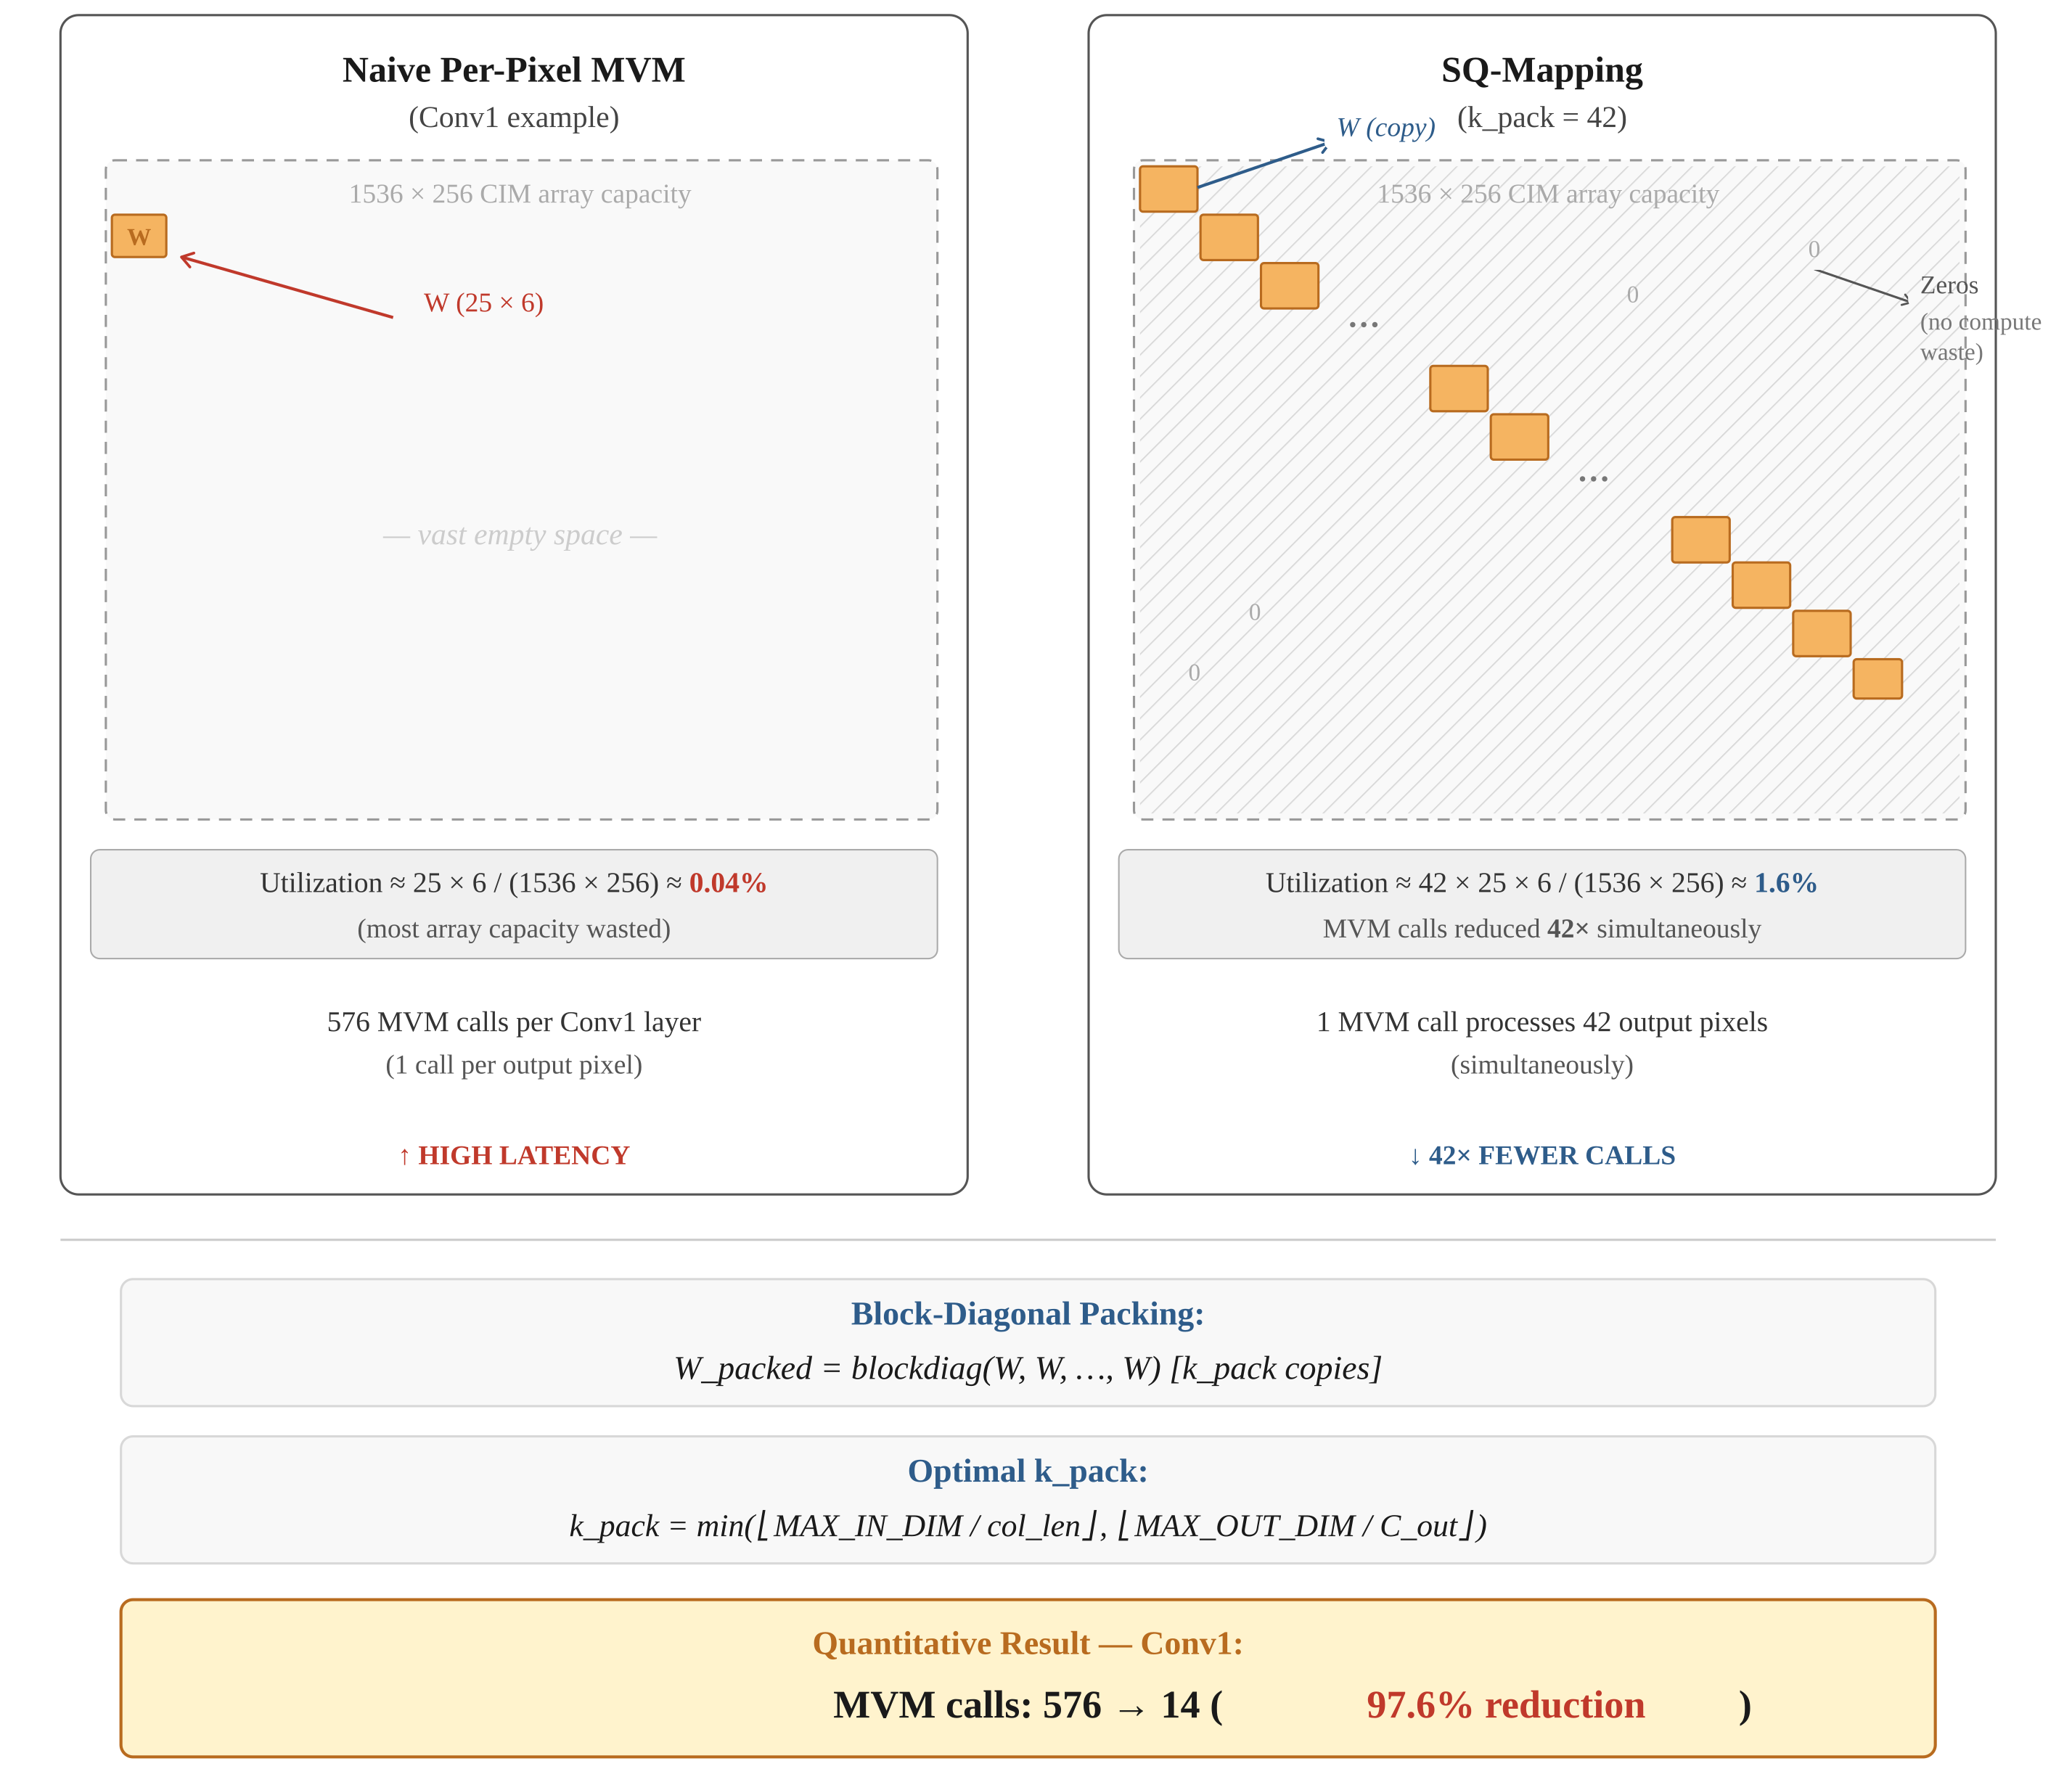
\includegraphics[width=\textwidth]{pics/4-5.png}
	\caption{SQ-mapping块对角权重打包示意图。左：逐像素MVM中$25\times6$权重塞入大阵列，利用率极低且每次调用开销无法均摊；右：沿对角线复制$k_{\text{pack}}$份权重构成块对角矩阵，单次MVM并行处理$k_{\text{pack}}$个输出像素，显著削减MVM调用次数。}
	\label{fig:sqmapping}
\end{figure}

\begin{table}[H]
	\centering
	\caption{LeNet-5卷积层SQ-mapping打包参数与效果}
	\label{tab:sqmapping}
	\small
	\begin{tabular}{lcccccc}
		\toprule
		层 & $\text{col\_len}$ & $C_{out}$ & $k_{\text{pack}}$ & 逐像素MVM次数 & 打包后MVM次数 & MVM削减比例 \\
		\midrule
		Conv1 & 25 & 6 & 42 & 576 & 14 & 97.6\% \\
		Conv2 & 150 & 16 & 10 & 64 & 7 & 89.1\% \\
		\bottomrule
	\end{tabular}
\end{table}

该优化不需要修改任何RTL，完全在Python驱动侧通过权重矩阵构造与输入向量拼接实现。启用SQ-mapping后，200张LeNet-5图片的逐层bit-exact验证全部通过，分类准确率仍为99.5\%（199/200），与逐像素调用模式完全一致。

\subsection{端到端性能分析}

\subsubsection{延迟分解}

表\ref{tab:latency_breakdown}给出了LeNet-5在最终配置（100 MHz，双缓冲乒乓，Layer Fusion，SQ-mapping，MAX\_IN\_DIM=1536）下200张图片的逐项延迟分解。

\begin{table}[H]
	\centering
	\caption{LeNet-5端到端延迟分解（200张MNIST，100 MHz，最终配置）}
	\label{tab:latency_breakdown}
	\small
	\begin{tabular}{lrr}
		\toprule
		阶段 & 延迟（ms/img） & 占比 \\
		\midrule
		MVM乒乓wall time（max(DMA, compute)） & 25.36 & 86.9\% \\
		im2col（向量化） & 1.22 & 4.2\% \\
		pool（向量化） & 1.24 & 4.2\% \\
		pack（预打包） & 0.66 & 2.3\% \\
		setup（摊薄） & 0.59 & 2.0\% \\
		final（argmax） & 0.11 & 0.4\% \\
		\midrule
		\textbf{合计} & \textbf{29.18} & \textbf{100\%} \\
		\bottomrule
	\end{tabular}
\end{table}

双缓冲乒乓机制已成功将DMA load\_x和read\_out隐藏在compute之后，当前的29.2 ms瓶颈实质上是所有MVM调用的乒乓wall time——即max(DMA传输时间, 硬件计算时间)的逐次累加。在此之后，不可重叠的Python侧开销（im2col + pool + pack + setup）合计约3.7 ms，仅占总延迟的12.7\%。图\ref{fig:latency_pie}以饼图形式直观呈现了该延迟分解。需要说明的是，上述逐项分解为profiler对单张图片的测量结果，各项合计约29.2 ms/幅，与表\ref{tab:arm_multi_model}中200张批量基准给出的29.91 ms/幅（33.4 fps）在逐次运行的波动范围内一致。

\begin{figure}[H]
	\centering
	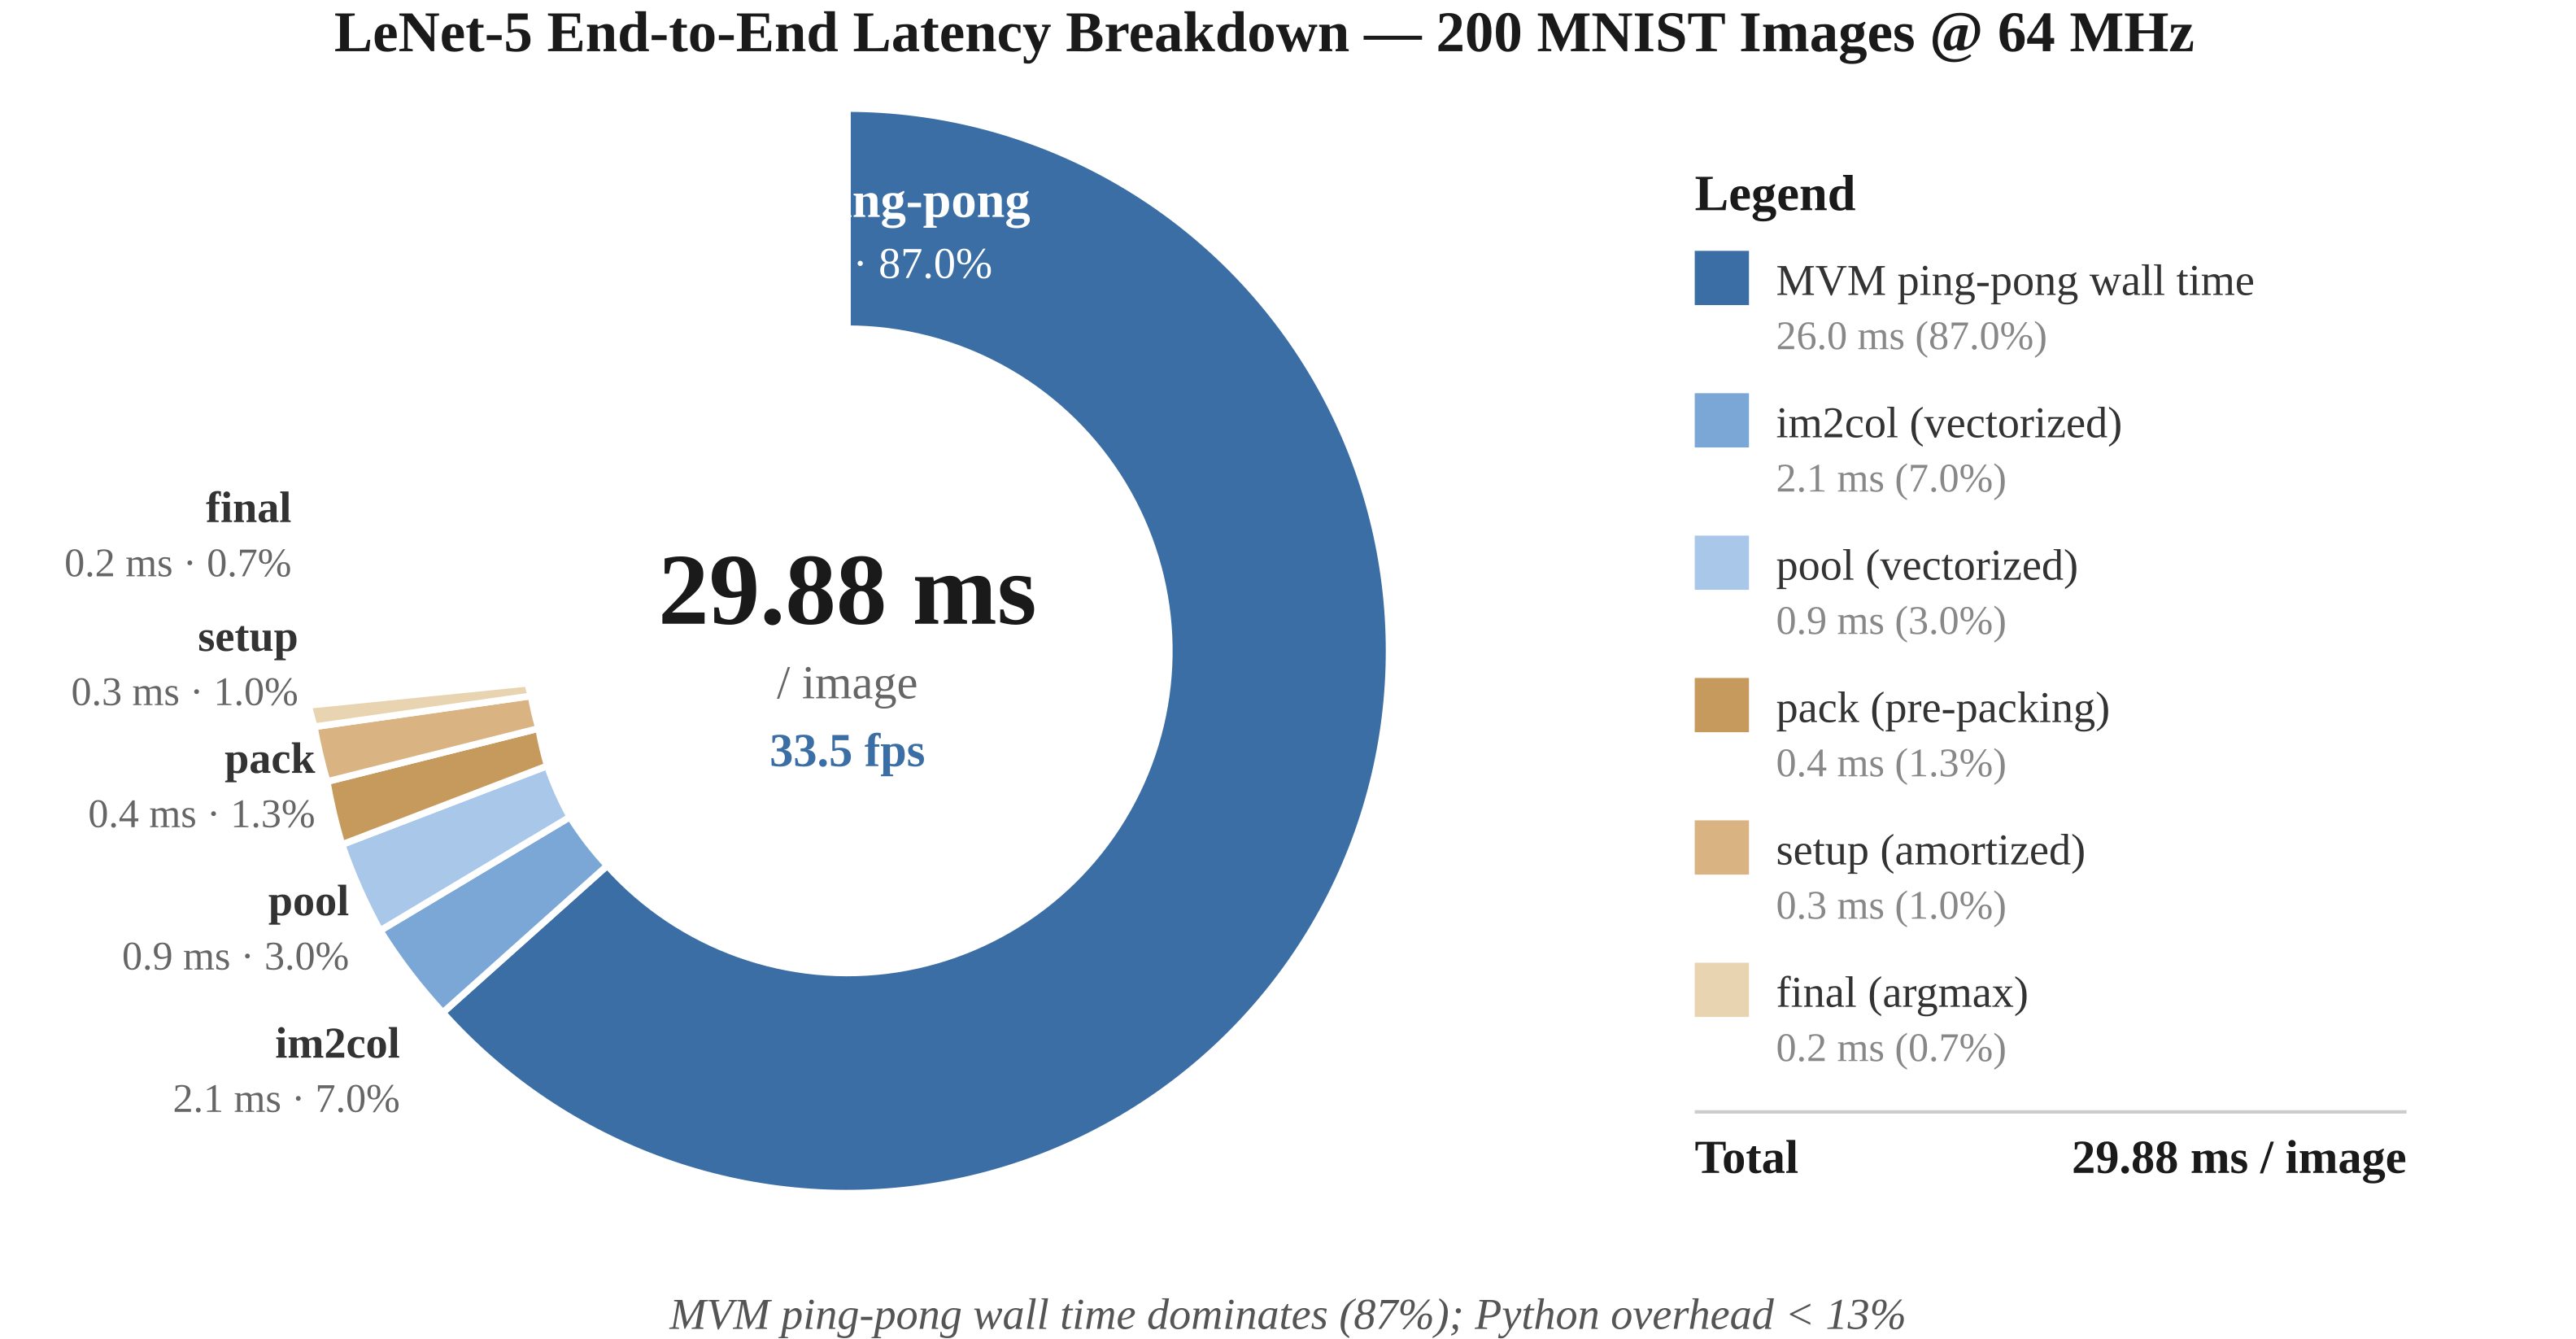
\includegraphics[width=0.72\textwidth]{pics/4-6.png}
	\caption{LeNet-5端到端延迟分解（200张MNIST，100 MHz，最终配置）。MVM乒乓wall time占86.9\%为绝对主导，im2col、pool、pack、setup与argmax等Python侧开销合计不足13\%。}
	\label{fig:latency_pie}
\end{figure}


\subsubsection{优化历程}

本设计的端到端性能经历了系统的优化过程，表\ref{tab:optimization_journey}以LeNet-5为例汇总了三种数据通路配置下的端到端延迟演进。三种配置均在统一的100 MHz工作频率与同一份CIM IP RTL下实测（数据取自表\ref{tab:arm_multi_model}中LeNet-5的MMIO/DMA/DMA+batch三行），阶段之间仅改变数据通路与批处理方式，因此累计加速比反映的是数据通路重构所带来的纯粹收益。优化路线遵循"先消除数据通路瓶颈，再隐藏剩余延迟"的策略：首先以AXI4-Stream + DMA双向数据通路替代逐字AXI4-Lite MMIO，从根本上消除数据搬运瓶颈；在此基础上，软件侧的SQ-mapping块对角权重打包（详见§\ref{sec:sqmapping}）提升了小卷积核场景下的CIM阵列利用率、削减了MVM调用次数；最后通过输入/输出双缓冲乒乓将DMA传输与硬件计算重叠，并利用Layer Fusion消除连续FC层间的S2MM+MM2S往返，结合批量推理摊薄逐图固定开销。

\begin{table}[H]
	\centering
	\caption{LeNet-5端到端优化历程（200张MNIST，PYNQ-Z2）}
	\label{tab:optimization_journey}
	\small
	\begin{tabular}{lccc}
		\toprule
		阶段 & 延迟（ms/img） & fps & 累计加速比 \\
		\midrule
		AXI4-Lite逐字MMIO基线 & 3261.06 & 0.31 & 1.0× \\
		\quad + AXI4-Stream/DMA双向数据通路 & 170.68 & 5.86 & 19.1× \\
		\quad + 双缓冲乒乓 + Layer Fusion + 批量推理 & \textbf{29.91} & \textbf{33.4} & \textbf{109×} \\
		\bottomrule
	\end{tabular}
\end{table}

从逐字MMIO基线到最终的DMA+批量配置，累计端到端加速比达到约\textbf{109倍}，吞吐率从0.31 fps提升至33.4 fps。最终配置分类准确率为99.5\%（199/200），各配置输出均与Python golden model逐元素bit-exact一致（一致率100\%）。该优化历程的延迟递减与累计加速比演进如图\ref{fig:opt_waterfall}所示。

\begin{figure}[H]
	\centering
	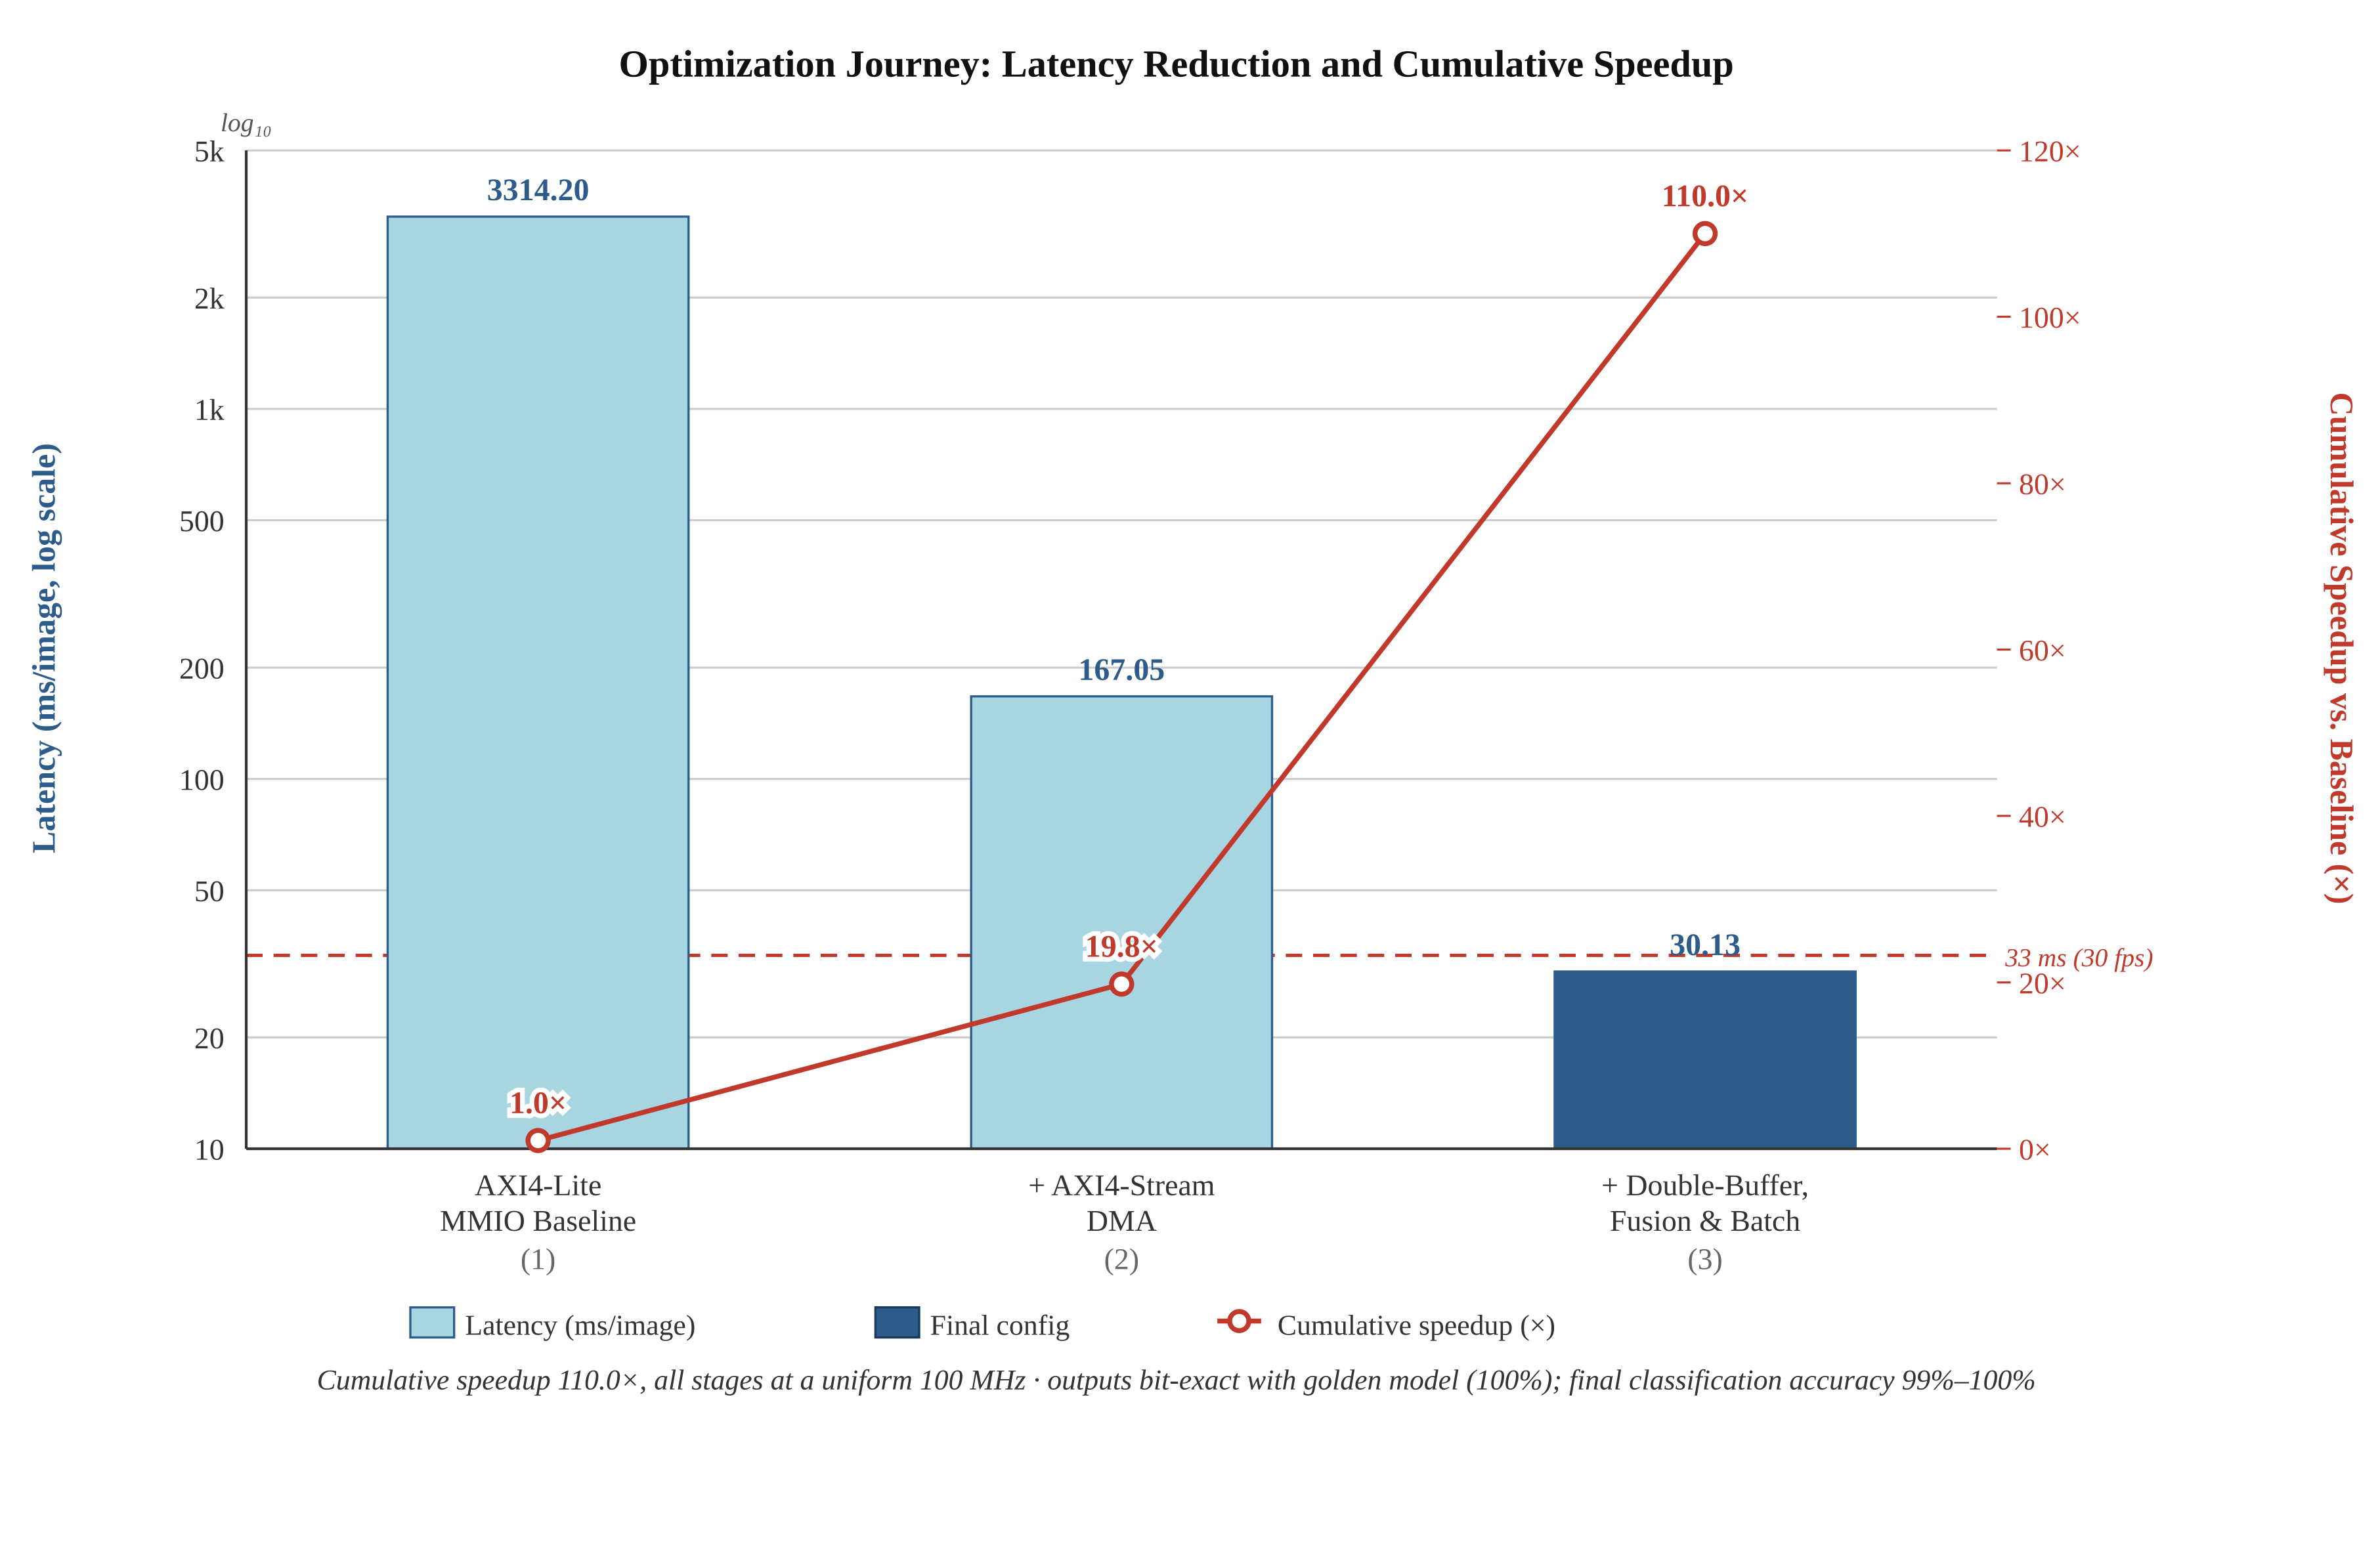
\includegraphics[width=0.92\textwidth]{pics/4-7.png}
	\caption{LeNet-5端到端优化历程瀑布图。柱状（左轴）为三种数据通路配置下延迟逐步下降，折线（右轴）为相对AXI4-Lite逐字MMIO基线的累计加速比，最终达到约109$\times$并越过30~fps实时阈值；各配置输出均与Python golden model逐元素bit-exact一致（一致率100\%），最终配置分类准确率99.5\%。}
	\label{fig:opt_waterfall}
\end{figure}

\subsection{加速比分析}

\subsubsection{硬件理论吞吐率}

CIM硬件的核心优势在于利用存储阵列的并行性实现高通量MAC运算。以FC1层（784→128）为例：

\begin{itemize}
	\item 总MAC操作数：$784 \times 128 = 100,352$
	\item 硬件周期数：3,136
	\item 每周期有效MAC数：$100352 / 3136 = 32$ MACs/cycle
	\item 吞吐率（100 MHz）：$32 \times 100 \times 10^6 = 3.20 \text{ GMACs/s}$
\end{itemize}

\subsubsection{软件基线对比}

表\ref{tab:speedup}给出了硬件推理与ARM Cortex-A9（650 MHz）纯NumPy软件基线的延迟对比。

\begin{table}[H]
	\centering
	\caption{SW基线与HW推理延迟对比（ARM Cortex-A9 @ 650 MHz vs CIM @ 100 MHz）}
	\begin{tabular}{lccc}
		\toprule
		网络 & SW延迟（$\mu$s） & HW延迟（$\mu$s） & 加速比 \\
		\midrule
		MLP（784→128→10） & 1,410.8 & 32.8 & \textbf{43.0×} \\
		LeNet-5（7层，sequential） & 26,466.2 & 760.3 & \textbf{34.8×} \\
		LeNet-5（7层，batched BLAS） & 4,528.5 & 760.3 & 6.0× \\
		\bottomrule
	\end{tabular}
	\label{tab:speedup}
\end{table}

MLP的SW延迟约1411 $\mu$s主要由FC1层（784×128，1368 $\mu$s）主导；HW延迟32.8 $\mu$s来自性能计数器实测3282周期，加速比约\textbf{43.0倍}。

LeNet-5的比较分两种模式：\textbf{sequential模式}与硬件相同地按输出像素逐一调用矩阵乘法（conv1 576次、conv2 64次），SW延迟约26.5 ms，加速比约\textbf{34.8倍}；\textbf{batched模式}将所有像素合并为单次矩阵乘法调用（BLAS路径），SW延迟约4.5 ms，加速比约6.0倍。Sequential模式是更公平的对比（与硬件计算模式等价），batched模式代表充分利用ARM CPU的最优SW实现上界。两种模式下CIM硬件均具有明显加速优势，对比结果如图\ref{fig:sw_vs_hw}所示。

\begin{figure}[H]
	\centering
	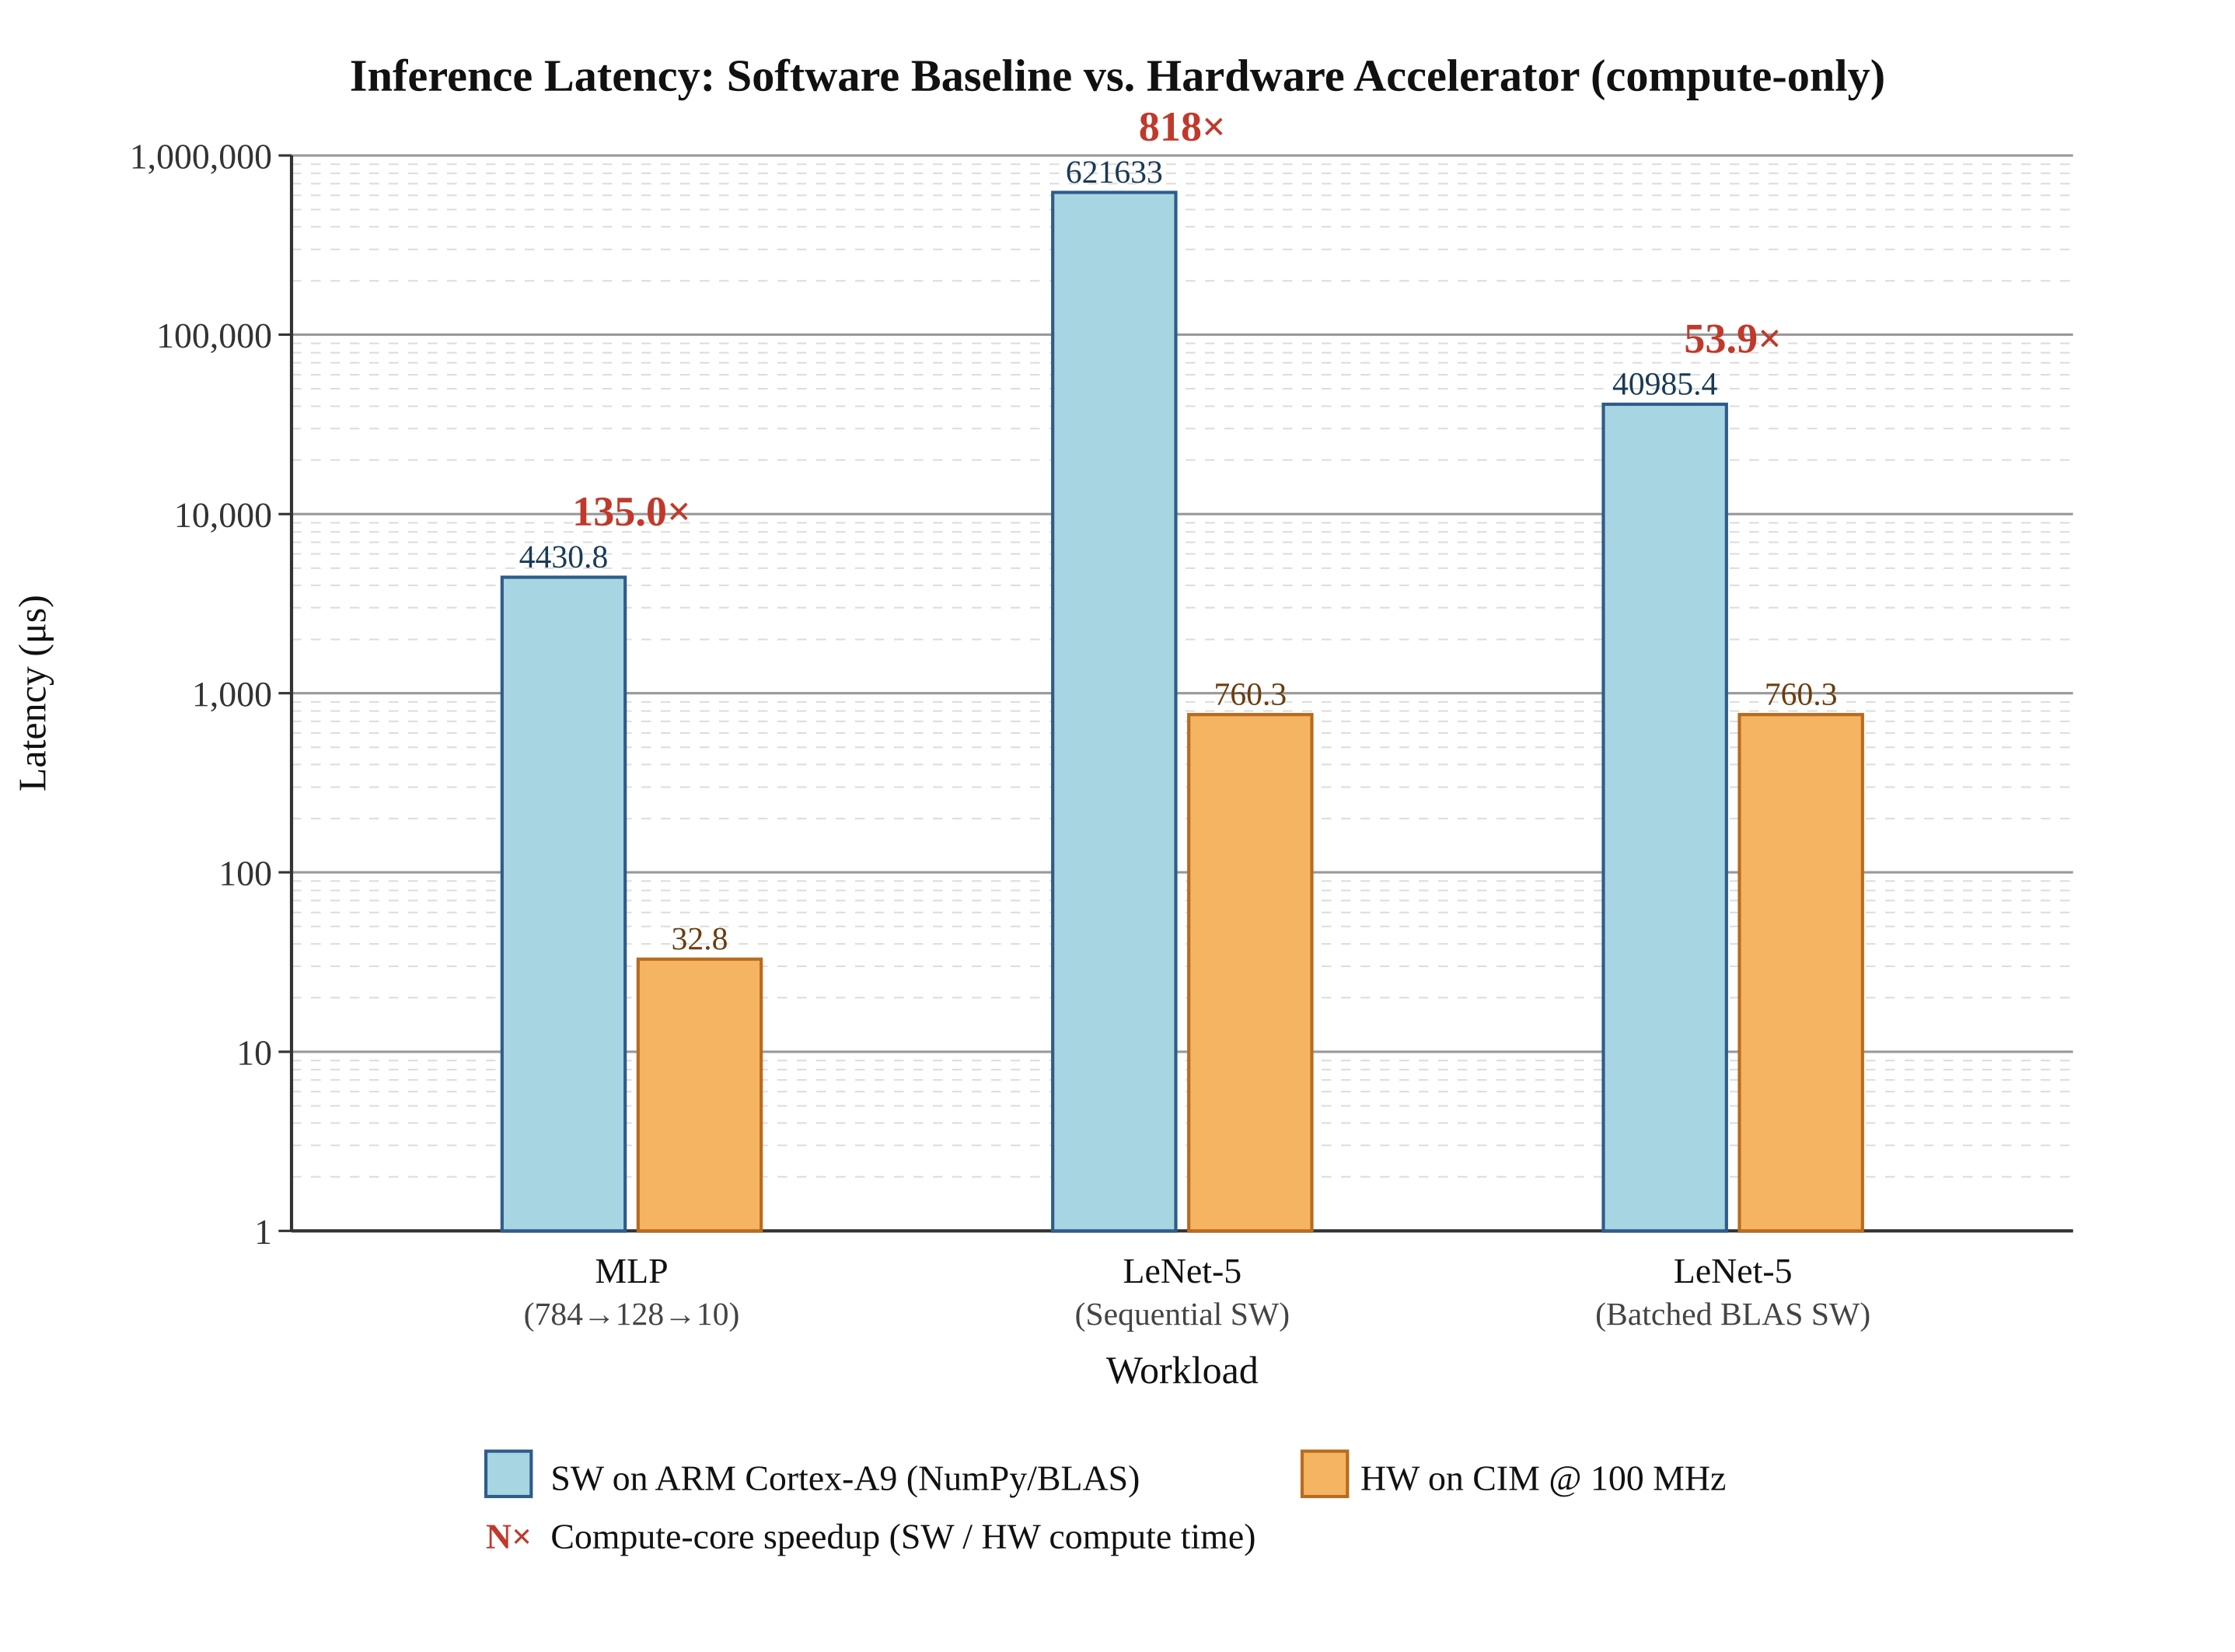
\includegraphics[width=0.85\textwidth]{pics/4-8.png}
	\caption{软件基线与硬件推理延迟对比（对数坐标，ARM Cortex-A9 @ 650 MHz vs CIM @ 100 MHz）。MLP、LeNet-5（sequential）、LeNet-5（batched）三组工作负载的加速比分别为43.0$\times$、34.8$\times$与6.0$\times$。}
	\label{fig:sw_vs_hw}
\end{figure}


\subsubsection{多模型多配置ARM端到端性能汇总}

表\ref{tab:arm_multi_model}汇总了ARM控制模式下三种网络（small\_mlp 784→16→10、MLP 784→128→10、LeNet-5）在三种数据通路配置（MMIO-only、DMA、DMA+batch）下的200张端到端实测性能。

\begin{table}[H]
	\centering
	\caption{ARM模式多模型多配置端到端性能汇总（100 MHz，200张MNIST）}
	\label{tab:arm_multi_model}
	\small
	\begin{tabular}{llcccc}
		\toprule
		模型 & 配置 & 总时间（s） & ms/img & fps & 准确率 \\
		\midrule
		\multirow{3}{*}{small\_mlp（784→16→10）} & MMIO & 16.20 & 81.00 & 12.3 & 96.50\% \\
		& DMA & 1.40 & 7.00 & 142.9 & 96.50\% \\
		& DMA+batch & \textbf{0.39} & \textbf{1.93} & \textbf{519.3} & 96.50\% \\
		\midrule
		\multirow{3}{*}{MLP（784→128→10）} & MMIO & 99.68 & 498.41 & 2.0 & 99.00\% \\
		& DMA & 5.59 & 27.93 & 35.8 & 99.00\% \\
		& DMA+batch & \textbf{0.40} & \textbf{2.00} & \textbf{499.6} & 99.00\% \\
		\midrule
		\multirow{3}{*}{LeNet-5（7层）} & MMIO & 652.21 & 3,261.06 & 0.31 & 98.50\% \\
		& DMA & 34.14 & 170.68 & 5.86 & 99.50\% \\
		& DMA+batch & \textbf{5.98} & \textbf{29.91} & \textbf{33.4} & 99.50\% \\
		\bottomrule
	\end{tabular}
\end{table}

从表可见：（1）DMA相比MMIO的加速比随模型规模增大而增大——small\_mlp约11.6倍、MLP约17.8倍、LeNet-5约19.1倍，因数据搬运量越大DMA的批量优势越明显；（2）DMA+batch（双缓冲乒乓+层融合）在DMA基础上进一步加速约3.6至14倍（small\_mlp约3.6倍、LeNet-5约5.7倍、MLP约14倍），将数据搬运延迟隐藏在计算之后；（3）各配置的硬件输出与Python golden model始终保持逐元素bit-exact一致（一致率100\%），即数据通路重构不引入任何计算误差；表中分类准确率为INT8量化模型相对标签的分类精度，由模型量化本身决定，与硬件数据通路无关。

\subsection{PicoRV32验证结果}

PicoRV32模式在PYNQ-Z2上使用100 MHz时钟（10 ns约束），WNS=$-$0.694 ns（592个failing endpoint，与ARM模式同属marginal时序，常温上板功能正常）。表\ref{tab:util_rv32}列出了该模式下的资源占用情况。

\begin{table}[H]
	\centering
	\caption{PicoRV32模式资源占用（PYNQ-Z2）}
	\begin{tabular}{lcccc}
		\toprule
		资源类型 & 使用量 & 可用量 & 占用率 & 相对ARM模式增量 \\
		\midrule
		Slice LUT & 17,023 & 53,200 & 32.00\% & $-$351 \\
		Slice Register & 8,594 & 106,400 & 8.08\% & $-$2,317 \\
		Block RAM & 129.5 & 140 & 92.50\% & +6 \\
		DSP48E1 & 220 & 220 & 100.00\% & +0 \\
		\bottomrule
	\end{tabular}
	\label{tab:util_rv32}
\end{table}

PicoRV32模式相比ARM模式的变化为：LUT减少351个、FF减少2,317个（因去除了axi\_dma及关联AXI Stream/Interconnect IP，代之以更轻量的PicoRV32核心约1,500 LUT + bridge + UART TX），BRAM增加6个（FW BRAM 32KB + Result BRAM 256B，共享部分CIM原有BRAM）。总体而言，PicoRV32模式以更少的逻辑资源实现了纯PL侧自主推理，代价是额外BRAM存储与模型规模受限。DSP使用量不变（均为220/220=100\%），因为CIM IP本身未修改。

\subsubsection{PicoRV32功能验证}

在PYNQ-Z2上针对784→16→10小型MLP模型（INT8量化，模型数据约14.5KB）进行了200张MNIST手写数字图片的端到端推理验证，结果如表\ref{tab:rv32_verify}所示。

\begin{table}[H]
	\centering
	\caption{PicoRV32推理验证结果（784→16→10 MLP，200张MNIST图片）}
	\begin{tabular}{lc}
		\toprule
		指标 & 值 \\
		\midrule
		测试图片数 & 200 \\
		分类准确率（vs 标签） & 96.50\%（193/200） \\
		Bit-exact一致率（vs Python golden） & 100.0\%（200/200） \\
		计算错误数 & 0 \\
		\bottomrule
	\end{tabular}
	\label{tab:rv32_verify}
\end{table}

200张图片的全部10维logits输出均与ARM控制模式下相同模型的预测结果完全一致（bit-exact），计算错误为零。7张分类错误均源于784→16→10模型自身的INT8量化精度损失（该模型INT8准确率约95.1\%，200张实测96.50\%），验证了RISC-V固件控制逻辑的正确性。

PicoRV32模式在small\_mlp（784→16→10）上的端到端实测性能为：总时间2.35 s（200张），平均11.74 ms/img（85.2 fps），准确率96.50\%（193/200），全部logits与ARM路径bit-exact一致。相比ARM模式下相同模型的DMA+batch配置（1.93 ms/img），PicoRV32的延迟约为6.1倍，主要差距来自PicoRV32缺少DMA批量传输能力——权重与输入数据需由CPU逐字写入CIM CSR（等效于ARM MMIO路径），而非通过AXI-Stream DMA批量搬运。该差距是控制路径（轻量RISC-V软核 vs ARM Cortex-A9 + DMA引擎）的固有差异，而非CIM计算核心的性能差异。事实上，两种模式运行的是同一份CIM IP RTL，对同一small\_mlp模型的硬件MVM计算周期数完全相同，端到端差异完全来自数据搬运方式。

\subsection{两种控制模式对比}

\begin{table}[H]
	\centering
	\caption{ARM控制 vs PicoRV32控制模式对比}
	\begin{tabular}{lcc}
		\toprule
		指标 & ARM控制 & PicoRV32控制 \\
		\midrule
		时钟频率 & 100 MHz & 100 MHz \\
		时序收敛 & WNS=$-$0.911 ns（marginal） & WNS=$-$0.694 ns（marginal） \\
		LUT占用 & 17,374 (32.66\%) & 17,023 (32.00\%) \\
		BRAM占用 & 123.5 (88.21\%) & 129.5 (92.50\%) \\
		small\_mlp延迟 & 1.93 ms/img（DMA+batch） & 11.74 ms/img \\
		small\_mlp吞吐 & 519.3 fps & 85.2 fps \\
		PS依赖 & 需要ARM PS运行Python & PS仅用于固件加载 \\
		支持网络 & 任意（受MAX\_DIM限制） & 受FW BRAM 32KB限制 \\
		CIM IP修改 & -- & 无修改 \\
		\bottomrule
	\end{tabular}
\end{table}


两种模式均工作于100 MHz且共享相同的CIM IP RTL。ARM模式在绝对性能上领先（受益于DMA批量数据传输），但PicoRV32模式展现出显著的轻量化优势——尽管集成了完整的32位RISC-V处理器、总线桥接与双端口BRAM，总LUT占用（17,023）反而低于ARM模式（17,374），FF更是减少了21.2\%（8,594 vs 10,911）。这一"做加法反得减法"的结果源于RISC-V软核（约1,500 LUT）远小于ARM模式所需的axi\_dma IP、AXI4-Stream sink/source及额外AXI互连的总开销。PicoRV32以更少的逻辑资源实现了纯PL侧自主推理，对小模型的推理延迟已处于实用范围（small\_mlp 11.74 ms/img，85.2 fps）。无论控制源为何，CIM IP在两种模式下完全相同，且计算结果bit-exact一致。

% ====================================================================
\section{总结与展望}
% ====================================================================

\subsection{工作总结}

本文设计并实现了一种面向边缘智能推理的Int8数字存算一体矩阵计算阵列架构，在PYNQ-Z2（Zynq-7020）FPGA平台上完成了完整的综合部署与板级验证。主要成果总结如下：

（1）\textbf{架构设计}：以16×16 CIM Tile为原子计算单元，设计了包含多级流水线的核心加速器引擎，支持通过CSR在运行时配置任意层维度与量化参数。所有设计参数集中管理于cim\_pkg.sv，实现了模块化、参数化的RTL框架。

（2）\textbf{数据通路优化}：设计了AXI4-Stream + DMA双向批量传输架构，将数据搬运从逐字MMIO替换为DMA批量传输；实现了输入/输出缓冲双bank乒乓结构，将DMA传输与硬件计算重叠执行；针对连续FC层设计了OBUF→IBUF内部硬件直拷的层融合机制，消除层间DMA往返。累计将LeNet-5端到端延迟从3,261.06 ms/img降至29.91 ms/img（约109×加速，33.4 fps）。

（3）\textbf{软件映射优化}：引入并适配了块对角权重打包（SQ-mapping）这一已有的卷积映射方法，通过将多个输出像素的im2col列合并到同一次MVM调用，将小卷积核场景下的阵列利用率提升至接近100\%，MVM调用次数削减89\%以上。同时通过im2col/MaxPool向量化、layer-wise批量化等手段将Python侧开销压缩至总延迟的12.7\%。

（4）\textbf{工程问题解决}：针对Vivado BRAM推断失败问题，通过16-bank权重SRAM拆分解决；针对关键路径时序违例，通过TILE\_SPLIT\_FACTOR流水拆分与后量化路径两级流水将时序收敛从60 MHz提升至80 MHz（完全收敛）和100 MHz（功能正确）。

（5）\textbf{软核集成与轻量化}：成功集成PicoRV32 RISC-V软核替代ARM PS进行推理控制，CIM IP完全不修改。相比ARM模式，PicoRV32模式展现出反直觉的轻量化优势：总LUT减少351个（17,023 vs 17,374）、FF减少2,317个（8,594 vs 10,911），仅BRAM增加6个（FW/Result双端口BRAM），以100 MHz时序收敛（WNS=$-$0.694 ns）。这一结果说明用轻量RISC-V软核（约1,500 LUT）替代复杂的DMA IP及关联Stream/Interconnect（合计超5,000 LUT/FF）是资源效率更优的纯PL推理方案。200张MNIST图片验证准确率96.50\%（193/200），全部logits与ARM路径bit-exact一致。

（6）\textbf{验证完备性}：建立了"Python golden model → VCS仿真 → PYNQ上板"三层一致的验证流程。MLP网络200张图片分类准确率99.0\%、LeNet-5 CNN 200张图片99.5\%（二者与golden model均100\% bit-exact一致）。所有优化阶段的硬件输出均与golden model保持100\% bit-exact一致；各配置的分类准确率取决于INT8量化模型本身（见表\ref{tab:arm_multi_model}）。

\subsection{不足与展望}
\label{sec:future_work}

（1）\textbf{DSP占用率}：当前设计DSP48E1占用率达到100\%，限制了并行度（PAR\_OB）的进一步提升。后续可通过DSP48 INT8×2 SIMD打包技术（利用单DSP的25×18乘法器同时计算两个独立INT8乘法，将DSP用量减半）释放资源用于PAR\_OB=2扩展，预期可将硬件compute吞吐再提升一倍。

（2）\textbf{最大维度限制}：当前MAX\_IN\_DIM=1536、MAX\_OUT\_DIM=256的配置已使BRAM占用率达88.2\%（PYNQ-Z2物理极限），适用于MNIST尺度网络但无法支持CIFAR-10/ImageNet级别模型。后续需通过权重分片加载（超标层分多次加载，消除维度硬上限）或迁移至更大BRAM容量的平台来解决。

（3）\textbf{更复杂网络与算子支持}：当前系统已支持Conv + FC + ReLU + MaxPool组成的网络，但尚未实现AveragePool、BatchNorm、Softmax等操作以及Depthwise Convolution、Residual Connection等结构。BatchNorm可在量化阶段静态折叠入权重与偏置（RTL零改动），MaxPool硬件化可进一步消除当前约1.24 ms的Python侧开销。

（4）\textbf{面向成熟推理框架的集成}：当前Python驱动需要为每个网络手动编写im2col与层调度逻辑，扩展到新模型的工程成本较高。未来可将CIM硬件抽象为ONNX Runtime的自定义执行后端，仅需在卷积/全连接算子内部注册硬件调用接口，即可复用成熟推理框架的完整前端图优化与算子调度能力，一次性获得YOLO、MobileNet、SqueezeNet等主流网络的支持。

（5）\textbf{稀疏计算支持}：ReLU激活后的特征图典型稀疏度为40--60\%，当前设计对所有零值元素仍执行完整的MAC运算与数据搬运。通过结构化剪枝结合权重压缩传输、零值跳过FSM，可进一步降低有效计算量与DMA传输量。

（6）\textbf{设计自动化}：当前改变PAR\_OB等编译期参数依赖脚本以sed方式patch cim\_pkg.sv，缺乏优雅性。后续可考虑用Chisel或SpinalHDL等参数化硬件描述语言重构核心加速器，以trait形式声明层级参数，一次elaborate即可出多个配置版本，同时可利用其与Verilator的天然集成简化仿真流程。


% ====================================================================
\section{致\hspace{1em}谢}

本课题的研究工作是在梁峰老师的悉心指导下完成的，在此谨向梁老师致以最诚挚的感谢。特别感谢课题组师兄王泽宇在毕设项目中关于DMA优化方案给予的宝贵指导与帮助。同时感谢课题组各位同学在项目研发过程中给予的帮助与建议。
% ====================================================================
\section{附\hspace{1em}录}

本文所述INT8 CIM加速器的全部设计源码、仿真测试平台、Python驱动与量化工具链、PicoRV32固件及FPGA综合脚本均可通过以下地址获取：

\begin{center}
\url{https://github.com/Invoker-pray/INT8-CIM-of-jiao}
\end{center}

仓库目录结构(master分支)如下：

\begin{itemize}
\item \texttt{hw/rtl/} — SystemVerilog RTL源码（CIM Tile、加速器核心、存储子系统、AXI接口）
\item \texttt{hw/tb/} — VCS仿真测试平台（Tile单元测试、系统MVM测试、MNIST端到端测试）
\item \texttt{hw/scripts/} — 仿真与综合脚本
\item \texttt{sw/} — Python驱动、量化工具链、golden model与板级benchmark
\item \texttt{picorv32/} — PicoRV32软核集成（RTL封装、固件、仿真与综合）
\item \texttt{vivado\_proj\_100mhz\_pynq/} — ARM控制模式Vivado工程（PYNQ-Z2，100 MHz）
\item \texttt{picorv32/vivado\_proj/} — PicoRV32控制模式Vivado工程（PYNQ-Z2，100 MHz）
\item \texttt{Thesis/end/paper/data/} — 板级实测benchmark原始数据（CSV格式）
\end{itemize}
% ====================================================================
% ====================================================================
\section{参考文献}
% ====================================================================
\nocite{*}
\printbibliography[heading=none]

\end{document}
